\documentclass[8pt]{beamer}

\usepackage[meeting={CTA Consortium Meeting},
            date={La Palma, 2017-11-06},
            title={The CTA pipepline prototype},
            shorttitle={ctapipe}]{beamersetup}

\usepackage{wasysym}

\begin{document}

    \begin{frame}
        \titlepage
    \end{frame}



    \begin{frame}{Introduction}
        \begin{itemize}
            \item[] the whole pipeline is up and running; cover here:
            \item image cleaning (tailcuts vs. wavelets)
            \item shower direction and impact reconstruction (purely geometric approach)
            \item $h_\mathrm{max}$ estimate (numerical minimisation in 3D)
            \item energy reconstruction (machine learning)
            \item event discrimination (machine learning)
            \item point-source sensitivity
            \item[]
            \item my github: \url{https://github.com/tino-michael/tino_cta}
            \item still needs external libraries for wavelet cleaning
        \end{itemize}

    \end{frame}


    \begin{frame}{Array Layout}
        \begin{columns}
            \column{.6\textwidth}
                \setlength{\figureheight}{\textwidth}
                \setlength{\figurewidth}{\textwidth}
                % This file was created by matplotlib2tikz v0.6.13.
\begin{tikzpicture}

\definecolor{color0}{rgb}{0.12156862745098,0.466666666666667,0.705882352941177}
\definecolor{color1}{rgb}{1,0.498039215686275,0.0549019607843137}
\definecolor{color2}{rgb}{0.172549019607843,0.627450980392157,0.172549019607843}

\begin{axis}[
title={HB9 L+N+D},
xlabel={$x / \mathrm{m}$},
ylabel={$y / \mathrm{m}$},
xtick={-1200,-800,...,1200},
ytick={-1200,-800,...,1200},
xmin=-1500, xmax=1500,
ymin=-1500, ymax=1500,
width=\figurewidth,
height=\figureheight,
tick align=outside,
tick pos=left,
x grid style={lightgray!92.026143790849673!black},
y grid style={lightgray!92.026143790849673!black},
legend style={draw=white!80.0!black,opacity=.75},
legend entries={{LST:LSTCam},{MST:NectarCam},{SST-1M:DigiCam}},
legend cell align={left}
]
\addplot [only marks, draw=color0, fill=color0, opacity=0.5, colormap/viridis, visualization depends on={\thisrow{sizedata} \as\perpointmarksize}, scatter/@pre marker code/.append style={/tikz/mark size=\perpointmarksize}]
table{%
x                      y                      sizedata
-2.000000000000000e+01 +6.500000000000000e+01 +5.315394051150731e+00
-2.000000000000000e+01 -6.500000000000000e+01 +5.315394051150731e+00
+8.000000000000000e+01 +0.000000000000000e+00 +5.315394051150731e+00
-1.200000000000000e+02 +0.000000000000000e+00 +5.315394051150731e+00
};
\addplot [only marks, draw=color1, fill=color1, opacity=0.5, colormap/viridis, visualization depends on={\thisrow{sizedata} \as\perpointmarksize}, scatter/@pre marker code/.append style={/tikz/mark size=\perpointmarksize}]
table{%
x                      y                      sizedata
+0.000000000000000e+00 +0.000000000000000e+00 +3.826166692590998e+00
+0.000000000000000e+00 +1.511999969482422e+02 +3.826166692590998e+00
+0.000000000000000e+00 -1.511999969482422e+02 +3.826166692590998e+00
+1.466559906005859e+02 +7.559999847412109e+01 +3.826166692590998e+00
+1.466559906005859e+02 -7.559999847412109e+01 +3.826166692590998e+00
-1.466559906005859e+02 +8.559999847412109e+01 +3.826166692590998e+00
-1.466559906005859e+02 -8.559999847412109e+01 +3.826166692590998e+00
+1.542050018310547e+02 +2.384739990234375e+02 +3.826166692590998e+00
+1.542050018310547e+02 -2.384739990234375e+02 +3.826166692590998e+00
+3.084100036621094e+02 +0.000000000000000e+00 +3.826166692590998e+00
-1.542050018310547e+02 +2.384739990234375e+02 +3.826166692590998e+00
-1.542050018310547e+02 -2.384739990234375e+02 +3.826166692590998e+00
-3.084100036621094e+02 +0.000000000000000e+00 +3.826166692590998e+00
+0.000000000000000e+00 +3.252420043945312e+02 +3.826166692590998e+00
+0.000000000000000e+00 -3.252420043945312e+02 +3.826166692590998e+00
+3.154680175781250e+02 +1.626210021972656e+02 +3.826166692590998e+00
+3.154680175781250e+02 -1.626210021972656e+02 +3.826166692590998e+00
-3.154680175781250e+02 +1.626210021972656e+02 +3.826166692590998e+00
-3.154680175781250e+02 -1.626210021972656e+02 +3.826166692590998e+00
+2.910849914550781e+02 +4.501549987792969e+02 +3.826166692590998e+00
+2.910849914550781e+02 -4.501549987792969e+02 +3.826166692590998e+00
+5.821699829101562e+02 +0.000000000000000e+00 +3.826166692590998e+00
-2.910849914550781e+02 +4.501549987792969e+02 +3.826166692590998e+00
-2.910849914550781e+02 -4.501549987792969e+02 +3.826166692590998e+00
-5.821699829101562e+02 +0.000000000000000e+00 +3.826166692590998e+00
};
\addplot [only marks, draw=color2, fill=color2, opacity=0.5, colormap/viridis, visualization depends on={\thisrow{sizedata} \as\perpointmarksize}, scatter/@pre marker code/.append style={/tikz/mark size=\perpointmarksize}]
table{%
x                      y                      sizedata
+2.055000000000000e+02 +1.588999938964844e+02 +2.099777750102006e+00
+2.055000000000000e+02 -1.588999938964844e+02 +2.099777750102006e+00
-2.055000000000000e+02 +1.588999938964844e+02 +2.099777750102006e+00
-2.055000000000000e+02 -1.588999938964844e+02 +2.099777750102006e+00
+1.648230133056641e+02 +4.248239746093750e+02 +2.099777750102006e+00
+1.648230133056641e+02 -4.248239746093750e+02 +2.099777750102006e+00
-1.648230133056641e+02 +4.248239746093750e+02 +2.099777750102006e+00
-1.648230133056641e+02 -4.248239746093750e+02 +2.099777750102006e+00
+4.944689941406250e+02 +1.100000000000000e+02 +2.099777750102006e+00
+4.944689941406250e+02 -1.100000000000000e+02 +2.099777750102006e+00
-4.944689941406250e+02 +1.100000000000000e+02 +2.099777750102006e+00
-4.944689941406250e+02 -1.100000000000000e+02 +2.099777750102006e+00
+0.000000000000000e+00 +5.197949829101562e+02 +2.099777750102006e+00
+0.000000000000000e+00 -5.197949829101562e+02 +2.099777750102006e+00
+3.916060180664062e+02 +4.037389831542969e+02 +2.099777750102006e+00
+3.916060180664062e+02 -4.037389831542969e+02 +2.099777750102006e+00
-3.916060180664062e+02 +4.037389831542969e+02 +2.099777750102006e+00
-3.916060180664062e+02 -4.037389831542969e+02 +2.099777750102006e+00
+6.180729980468750e+02 +3.186109924316406e+02 +2.099777750102006e+00
+6.180729980468750e+02 -3.186109924316406e+02 +2.099777750102006e+00
-6.180729980468750e+02 +3.186109924316406e+02 +2.099777750102006e+00
-6.180729980468750e+02 -3.186109924316406e+02 +2.099777750102006e+00
+0.000000000000000e+00 +7.235270385742188e+02 +2.099777750102006e+00
+0.000000000000000e+00 -7.235270385742188e+02 +2.099777750102006e+00
+8.200000000000000e+02 +0.000000000000000e+00 +2.099777750102006e+00
-8.200000000000000e+02 +0.000000000000000e+00 +2.099777750102006e+00
+4.353039855957031e+02 +6.731860351562500e+02 +2.099777750102006e+00
+4.353039855957031e+02 -6.731860351562500e+02 +2.099777750102006e+00
-4.353039855957031e+02 +6.731860351562500e+02 +2.099777750102006e+00
-4.353039855957031e+02 -6.731860351562500e+02 +2.099777750102006e+00
+2.208440093994141e+02 +7.969029541015625e+02 +2.099777750102006e+00
+2.208440093994141e+02 -7.969029541015625e+02 +2.099777750102006e+00
+6.625329589843750e+02 +5.692160034179688e+02 +2.099777750102006e+00
+6.625329589843750e+02 -5.692160034179688e+02 +2.099777750102006e+00
+8.833770141601562e+02 +2.276869964599609e+02 +2.099777750102006e+00
+8.833770141601562e+02 -2.276869964599609e+02 +2.099777750102006e+00
-2.208440093994141e+02 +7.969029541015625e+02 +2.099777750102006e+00
-2.208440093994141e+02 -7.969029541015625e+02 +2.099777750102006e+00
-6.625329589843750e+02 +5.692160034179688e+02 +2.099777750102006e+00
-6.625329589843750e+02 -5.692160034179688e+02 +2.099777750102006e+00
-8.833770141601562e+02 +2.276869964599609e+02 +2.099777750102006e+00
-8.833770141601562e+02 -2.276869964599609e+02 +2.099777750102006e+00
+0.000000000000000e+00 +9.443010253906250e+02 +2.099777750102006e+00
+0.000000000000000e+00 -9.443010253906250e+02 +2.099777750102006e+00
+9.159229736328125e+02 +4.721510009765625e+02 +2.099777750102006e+00
+9.159229736328125e+02 -4.721510009765625e+02 +2.099777750102006e+00
-9.159229736328125e+02 +4.721510009765625e+02 +2.099777750102006e+00
-9.159229736328125e+02 -4.721510009765625e+02 +2.099777750102006e+00
+1.100000000000000e+03 +0.000000000000000e+00 +2.099777750102006e+00
-1.100000000000000e+03 +0.000000000000000e+00 +2.099777750102006e+00
+4.710119934082031e+02 +9.712100219726562e+02 +2.099777750102006e+00
+4.710119934082031e+02 -9.712100219726562e+02 +2.099777750102006e+00
+7.065179443359375e+02 +8.498089599609375e+02 +2.099777750102006e+00
+7.065179443359375e+02 -8.498089599609375e+02 +2.099777750102006e+00
-4.710119934082031e+02 +9.712100219726562e+02 +2.099777750102006e+00
-4.710119934082031e+02 -9.712100219726562e+02 +2.099777750102006e+00
-7.065179443359375e+02 +8.498089599609375e+02 +2.099777750102006e+00
-7.065179443359375e+02 -8.498089599609375e+02 +2.099777750102006e+00
+2.391969909667969e+02 +1.109734985351562e+03 +2.099777750102006e+00
+2.391969909667969e+02 -1.109734985351562e+03 +2.099777750102006e+00
+9.567870483398438e+02 +7.398229980468750e+02 +2.099777750102006e+00
+9.567870483398438e+02 -7.398229980468750e+02 +2.099777750102006e+00
-2.391969909667969e+02 +1.109734985351562e+03 +2.099777750102006e+00
-2.391969909667969e+02 -1.109734985351562e+03 +2.099777750102006e+00
-9.567870483398438e+02 +7.398229980468750e+02 +2.099777750102006e+00
-9.567870483398438e+02 -7.398229980468750e+02 +2.099777750102006e+00
+1.195984008789062e+03 +3.699119873046875e+02 +2.099777750102006e+00
+1.195984008789062e+03 -3.699119873046875e+02 +2.099777750102006e+00
-1.195984008789062e+03 +3.699119873046875e+02 +2.099777750102006e+00
-1.195984008789062e+03 -3.699119873046875e+02 +2.099777750102006e+00
};
\end{axis}

\end{tikzpicture}

            \column{.4\textwidth}
                \begin{itemize}
                    \item until recently, only running on ASTRI mini-array
                    \item now on full Paranal array:
                    \item HB9 layout\\ (LST + Nectar + DigiCam)
                    \item pointing north at \unit{20}{\degree}
                    \item on-axis gammas,\\ diffuse protons and electrons
                \end{itemize}
        \end{columns}
    \end{frame}


    \begin{frame}{Cleaning}
        \ \\
        \vfill
        \begin{columns}
            \column{.5\textwidth}
                \begin{itemize}
                    \item[] comparing two cleaning methods:
                    \item two-step tailcuts (implemented in ctapipe)
                    \item wavelet cleaning developed by Jérémie\\
                        (to be merged into ctapipe)\\\ %
%                     \item[]
                \end{itemize}
            \column{.5\textwidth}
                \begin{itemize}
                    \item[]
                    \item run the pipeline separately once for each cleaning method
                    \item i.e. each cleaning does its own ML training, reconstruction,
                        discrimination ...
                \end{itemize}
        \end{columns}
        \vfill
        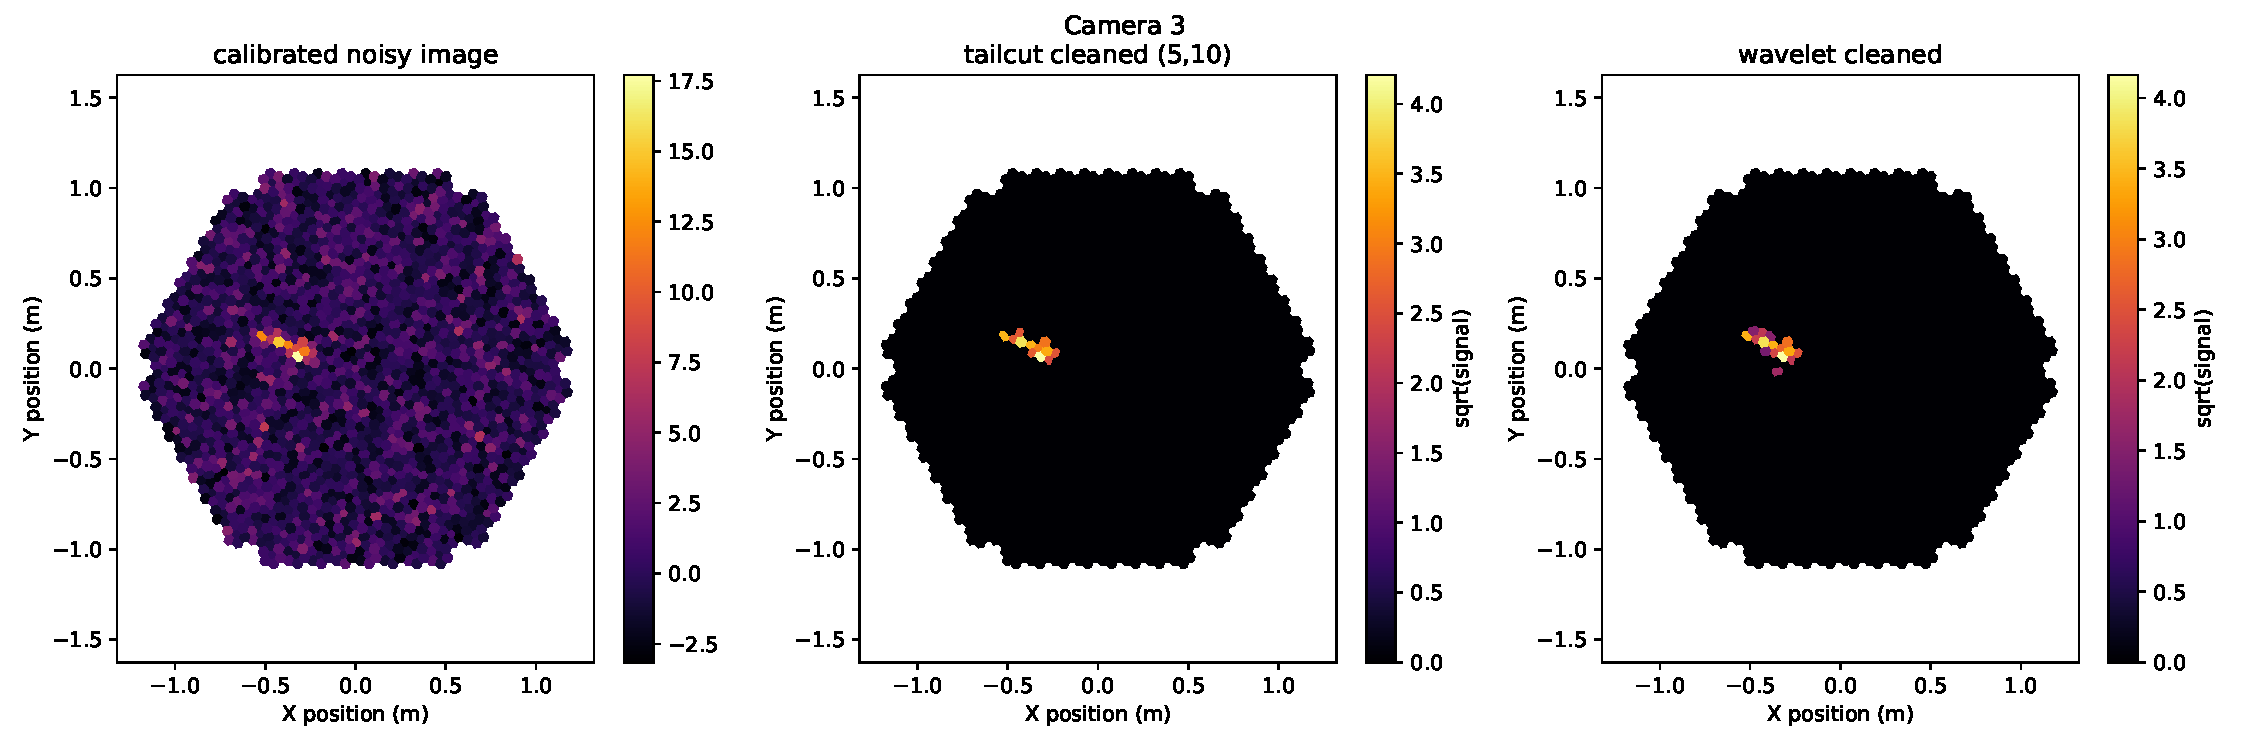
\includegraphics[width=\textwidth]{pics/camera_display_cleaning}
    \end{frame}


    \begin{frame}{simple shower-reco}{camera frame}
        \begin{columns}
            \column{.5\textwidth}
                \begin{itemize}
                    \item Hillas parametrisation provides several parameters:
                    \begin{itemize}
                        \item position of image core {\color{blue}$c$}
                        \item tilt of ellipsis $\psi$
                    \end{itemize}
                    \item $\rightarrow$ arbitrary point {\color{red}$b$} on shower axis
                    \item note that every pixel on the camera corresponds to a direction in the sky
                    \item $b$ and $c$ form a plane in which the shower lies
                \end{itemize}

            \column{.5\textwidth}
                \centering
                \begin{tikzpicture}
                    \node[base=center] (0,0) {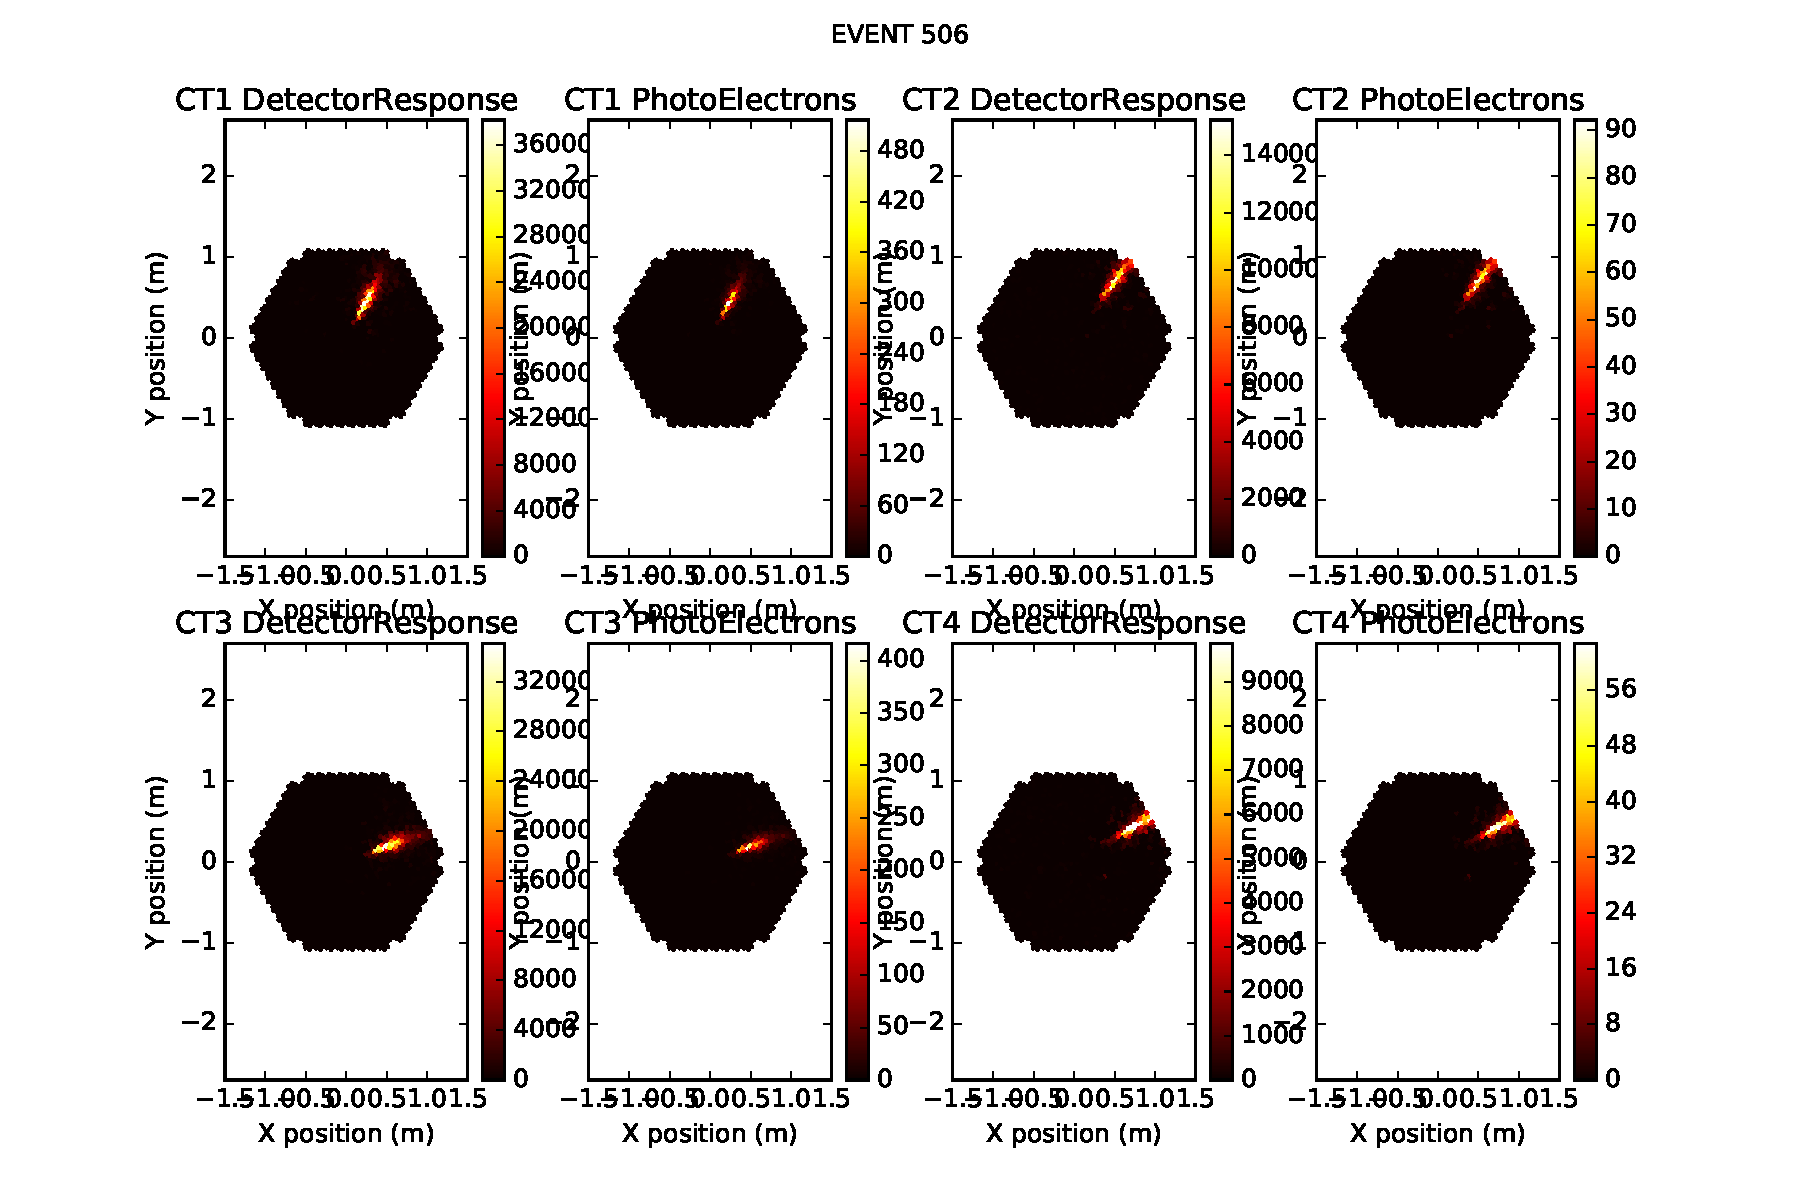
\includegraphics[trim=4cm 4cm 22.8cm 13cm, clip, width=4.5cm]{pics/display.pdf}};
                    \coordinate (shmax) at (.8,.4);

                    \draw[thick,white] (1.5,0) arc (0:25:1.5) node [midway,left,white] {$\psi$};

                    \foreach \P in {(shmax)}{\draw[mark options={color=blue!100!black},mark size=2.402402pt,very thick,mark=star] plot coordinates {\P} node[color=blue!50!white,shift=(120:.2)] {$c$};}
                    \foreach \P in {(25:1.5)}{\draw[mark options={color=red!100!black},mark size=2.402402pt,very thick,mark=star] plot coordinates {\P} node[color=red!50!white,shift=(120:.2)] {$b$};}
                    \draw[thick,white,-stealth] (0,0) -- +(25:1.8);
                \end{tikzpicture}
        \end{columns}
    \end{frame}



    \begin{frame}{simple shower-reco -- direction}{horizontal frame}
        \centering
        \begin{tikzpicture}
            \draw[-stealth] (.5,.5) -- +(5mm,0) node[below] {$x$};
            \draw[-stealth] (.5,.5) -- +(60:3.5mm) node[right] {$y$};
            \draw[-stealth] (.5,.5) -- +(0,5mm) node[left] {$z$};
            \draw[color=white] (0,0) rectangle (10,7);
            \coordinate (tel1) at (2,1);
            \draw[black,fill] (tel1) circle (.05) node[below] {Tel 1};
            \only<1->{
                \coordinate (a2) at ([yshift=3cm]tel1);
                \coordinate (a3) at ([xshift=6cm,yshift=1.5cm]a2);
                \coordinate (a4) at ([yshift=-3cm]a3);
                \draw[line width=0.3mm] (tel1) -- (a2) -- (a3) -- (a4) -- (tel1);
            }
            \only<2->{
                \coordinate (tel2) at (8.5,1);
                \draw[black,fill] (tel2) circle (.05) node[below] {Tel 2};
                \coordinate (b2) at ([yshift=3cm]tel2);
                \coordinate (b3) at ([xshift=-6cm,yshift=1.5cm]b2);
                \coordinate (b4) at ([yshift=-3cm]b3);
                \draw[line width=0.3mm] (tel2) -- (b2) -- (b3) -- (b4) -- (tel2);

                \path[name path=line1low] (tel1) -- (a4);
                \path[name path=line1hig] (a2) -- (a3);
                \path[name path=line2low] (tel2) -- (b4);
                \path[name path=line2hig] (b2) -- (b3);

                \path[name intersections={of = line1low and line2low}];
                \coordinate (sel12low) at (intersection-1);
                \path[name intersections={of = line1hig and line2hig}];
                \coordinate (sel12hig) at (intersection-1);
                \draw[line width=.7mm] (sel12hig) -- (sel12low);
            }
            \only<3>{
                \draw[thick,-stealth,shorten >=.1cm]
                    (8,6.2) -- ( $(sel12hig) !.3! (sel12low)$ );
                \node[anchor=south east] at (10,6.25)
                    {orientation of this cross section is the shower direction!};
            }
            \only<4->{
                \coordinate (tel3) at (7,3);
                \draw[black,fill] (tel3) circle (.05) node[right] {Tel 3};
                \coordinate (c2) at ([yshift=3cm]tel3);
                \coordinate (c3) at ([xshift=-4cm,yshift=-2.2cm]c2);
                \coordinate (c4) at ([yshift=-3cm]c3);
                \draw[line width=0.3mm] (tel3) -- (c2) -- (c3) -- (c4) -- (tel3);

                \path[name path=line3low] (tel3) -- (c4);
                \path[name path=line3hig] (c2) -- (c3);

                \path[name intersections={of = line1low and line3low}];
                \coordinate (sel13low) at (intersection-1);
                \path[name intersections={of = line1hig and line3hig}];
                \coordinate (sel13hig) at (intersection-1);
                \draw[line width=.7mm] (sel13hig) -- (sel13low);

                \path[name intersections={of = line2low and line3low}];
                \coordinate (sel23low) at (intersection-1);
                \path[name intersections={of = line2hig and line3hig}];
                \coordinate (sel23hig) at (intersection-1);
                \draw[line width=.7mm] (sel23hig) -- (sel23low);
                \node[anchor=south east] at (10,6.25)
                    {more cross sections means more direction estimators};
            }
        \end{tikzpicture}
    \end{frame}


    \begin{frame}{weighted mean direction of intersections}{implementation}
        \begin{itemize}
            \item this cross section is perpendicular to the normal direction of both
                intersecting planes ($\vec n = \vec b \times \vec c$)
            \item $\rightarrow$ shower direction is $\vec n_1 \times \vec n_2$
            \item add up all cross products for weighted mean direction:
                $$\vec d_\gamma = \sum_{i=1}^{N_\mathrm{Tels}}
                \sum_{j=i+1}^{N_\mathrm{Tels}} w_{ij} \cdot \vec n_i \times \vec n_j$$
            \item $w_{ij}$: weight containing the total image intensity\\
                and eccentricity of the Hillas ellipsis
            \item note: $|\vec n_i \times \vec n_j| = |\vec n_i| \cdot |\vec n_j| \cdot
                \sin[ \measuredangle(\vec n_i, \vec n_j )]$
            \item[] $\rightarrow$ automatically weights contributions according\\
                to the angle between intersecting planes
            \item[] $\rightarrow$ planes pairs crossing with more acute angle are
                weighted less
        \end{itemize}
    \end{frame}


    \begin{frame}{Shower Reconstruction -- Direction}
            {Angle between reconstructed and simulated direction}
        \setlength{\figureheight}{4.5cm}
        \setlength{\figurewidth}{10cm}
        \centering
        % This file was created by matplotlib2tikz v0.6.13.
\begin{tikzpicture}


\begin{groupplot}[group style={group size=1 by 2}]
\nextgroupplot[
xlabel={$N_\mathrm{Tels}$},
ylabel={$\log_{10}(\xi / ^\circ)$},
xmin=0, xmax=50,
ymin=-3, ymax=0.5,
width=\figurewidth,
height=\figureheight,
tick align=outside,
tick pos=left,
xmajorgrids,
x grid style={lightgray!92.026143790849673!black},
ymajorgrids,
y grid style={lightgray!92.026143790849673!black}
legend style={at={(0.99,0.99)}},
legend entries={wavelets, tail cuts}
]

\addlegendimage{line width=7pt,opacity=0.3,color=darkorange}
\addlegendimage{line width=7pt,opacity=0.3,color=darkred}


\path [fill=darkorange, fill opacity=0.3] (axis cs:2.5000,-4.71572539871238)
--(axis cs:2.49998649581333,-4.71572539871238)
--(axis cs:2.49999999856575,-4.60122823261679)
--(axis cs:2.49999999999999,-4.4867310665212)
--(axis cs:2.4999986857365,-4.3722339004256)
--(axis cs:2.4999985449655,-4.25773673433001)
--(axis cs:2.4999897089086,-4.14323956823442)
--(axis cs:2.49999470913709,-4.02874240213883)
--(axis cs:2.49998386494279,-3.91424523604324)
--(axis cs:2.49997924457232,-3.79974806994765)
--(axis cs:2.49997650676031,-3.68525090385206)
--(axis cs:2.49996824332969,-3.57075373775647)
--(axis cs:2.49994867052718,-3.45625657166088)
--(axis cs:2.49989461539032,-3.34175940556529)
--(axis cs:2.49983013668622,-3.2272622394697)
--(axis cs:2.49974655770429,-3.11276507337411)
--(axis cs:2.49960632222094,-2.99826790727852)
--(axis cs:2.49926272731697,-2.88377074118292)
--(axis cs:2.49895905168786,-2.76927357508733)
--(axis cs:2.49814115469221,-2.65477640899174)
--(axis cs:2.49680751915567,-2.54027924289615)
--(axis cs:2.4942637218094,-2.42578207680056)
--(axis cs:2.49010224556074,-2.31128491070497)
--(axis cs:2.48364209051371,-2.19678774460938)
--(axis cs:2.47287380044511,-2.08229057851379)
--(axis cs:2.45502277726056,-1.9677934124182)
--(axis cs:2.42323250885958,-1.85329624632261)
--(axis cs:2.37466163074462,-1.73879908022702)
--(axis cs:2.29638243604765,-1.62430191413143)
--(axis cs:2.17415938745622,-1.50980474803584)
--(axis cs:1.99721343861637,-1.39530758194024)
--(axis cs:1.7457149557578,-1.28081041584465)
--(axis cs:1.42650973295076,-1.16631324974906)
--(axis cs:1.08160848061456,-1.05181608365347)
--(axis cs:0.729139126802985,-0.937318917557882)
--(axis cs:0.429249985406498,-0.822821751462291)
--(axis cs:0.262743060469801,-0.7083245853667)
--(axis cs:0.25,-0.593827419271109)
--(axis cs:0.391029367601661,-0.479330253175519)
--(axis cs:0.661468284266056,-0.364833087079928)
--(axis cs:0.97904151844741,-0.250335920984337)
--(axis cs:1.32812609331274,-0.135838754888747)
--(axis cs:1.65198315722576,-0.0213415887931561)
--(axis cs:1.89594872419632,0.0931555773024346)
--(axis cs:2.06981080808935,0.207652743398025)
--(axis cs:2.18787301265835,0.322149909493616)
--(axis cs:2.27598839241379,0.436647075589208)
--(axis cs:2.33234566672976,0.551144241684798)
--(axis cs:2.37650778368071,0.665641407780389)
--(axis cs:2.4048553765849,0.78013857387598)
--(axis cs:2.42950704893189,0.89463573997157)
--(axis cs:2.44449041590275,1.00913290606716)
--(axis cs:2.45686551443184,1.12363007216275)
--(axis cs:2.46641927220215,1.23812723825834)
--(axis cs:2.47360191793967,1.35262440435393)
--(axis cs:2.47973224437672,1.46712157044952)
--(axis cs:2.48334339523982,1.58161873654511)
--(axis cs:2.48593453867151,1.69611590264071)
--(axis cs:2.48724007009689,1.8106130687363)
--(axis cs:2.49143970860728,1.92511023483189)
--(axis cs:2.49741789488778,2.03960740092748)
--(axis cs:2.50,2.03960740092748)
--cycle;

\path [fill=darkorange, fill opacity=0.3] (axis cs:7.5,-4.56542423372972)
--(axis cs:7.49996707711437,-4.56542423372972)
--(axis cs:7.49997769533599,-4.47072325171595)
--(axis cs:7.49994775204345,-4.37602226970219)
--(axis cs:7.49999941370705,-4.28132128768843)
--(axis cs:7.49999999999999,-4.18662030567466)
--(axis cs:7.5,-4.0919193236609)
--(axis cs:7.5,-3.99721834164713)
--(axis cs:7.49999985205654,-3.90251735963337)
--(axis cs:7.49995422619085,-3.8078163776196)
--(axis cs:7.49996678217128,-3.71311539560584)
--(axis cs:7.49995085879867,-3.61841441359207)
--(axis cs:7.49991740225088,-3.52371343157831)
--(axis cs:7.49977459698884,-3.42901244956454)
--(axis cs:7.49970178822804,-3.33431146755078)
--(axis cs:7.49943918177526,-3.23961048553701)
--(axis cs:7.49944198323576,-3.14490950352325)
--(axis cs:7.49903070430629,-3.05020852150948)
--(axis cs:7.49827370031703,-2.95550753949572)
--(axis cs:7.49722402215291,-2.86080655748196)
--(axis cs:7.49669241577257,-2.76610557546819)
--(axis cs:7.49419031927282,-2.67140459345443)
--(axis cs:7.49123989623413,-2.57670361144066)
--(axis cs:7.4868058759923,-2.4820026294269)
--(axis cs:7.47973845483072,-2.38730164741313)
--(axis cs:7.46756423436877,-2.29260066539937)
--(axis cs:7.45061463445017,-2.1978996833856)
--(axis cs:7.42119231942659,-2.10319870137184)
--(axis cs:7.38388935470011,-2.00849771935807)
--(axis cs:7.32969004233956,-1.91379673734431)
--(axis cs:7.24165133627961,-1.81909575533054)
--(axis cs:7.12175370725589,-1.72439477331678)
--(axis cs:6.9618252553736,-1.62969379130301)
--(axis cs:6.73872190760578,-1.53499280928925)
--(axis cs:6.47581809509833,-1.44029182727549)
--(axis cs:6.16671261760649,-1.34559084526172)
--(axis cs:5.86242772713057,-1.25088986324796)
--(axis cs:5.57343719638932,-1.15618888123419)
--(axis cs:5.36769488061328,-1.06148789922043)
--(axis cs:5.25,-0.966786917206662)
--(axis cs:5.27121653090323,-0.872085935192897)
--(axis cs:5.41813303154107,-0.777384953179133)
--(axis cs:5.73401565044382,-0.682683971165368)
--(axis cs:6.09494885552632,-0.587982989151603)
--(axis cs:6.4853459454683,-0.493282007137839)
--(axis cs:6.83238309715809,-0.398581025124074)
--(axis cs:7.10010783162486,-0.303880043110309)
--(axis cs:7.27787389358594,-0.209179061096544)
--(axis cs:7.38501538709966,-0.11447807908278)
--(axis cs:7.44993401502315,-0.0197770970690145)
--(axis cs:7.47496464630564,0.0749238849447496)
--(axis cs:7.48854705719207,0.169624866958515)
--(axis cs:7.49473698520916,0.264325848972279)
--(axis cs:7.49821247714115,0.359026830986044)
--(axis cs:7.49925082087896,0.453727812999809)
--(axis cs:7.49952101422211,0.548428795013573)
--(axis cs:7.49975031213014,0.643129777027338)
--(axis cs:7.4999166098842,0.737830759041103)
--(axis cs:7.49994614702737,0.832531741054867)
--(axis cs:7.49999926470388,0.927232723068632)
--(axis cs:7.49996707753512,1.0219337050824)
--(axis cs:7.5,1.0219337050824)
--cycle;

\path [fill=darkorange, fill opacity=0.3] (axis cs:12.5,-3.89868322400708)
--(axis cs:12.4998695380201,-3.89868322400708)
--(axis cs:12.4999615907455,-3.8235022257097)
--(axis cs:12.4999388475969,-3.74832122741233)
--(axis cs:12.4997636657388,-3.67314022911495)
--(axis cs:12.4998356253667,-3.59795923081758)
--(axis cs:12.4995585501396,-3.5227782325202)
--(axis cs:12.4995313942247,-3.44759723422283)
--(axis cs:12.4988645766383,-3.37241623592545)
--(axis cs:12.4990572726135,-3.29723523762808)
--(axis cs:12.498676292215,-3.2220542393307)
--(axis cs:12.4986212278887,-3.14687324103333)
--(axis cs:12.4981360486902,-3.07169224273595)
--(axis cs:12.4968680202255,-2.99651124443858)
--(axis cs:12.4952332518351,-2.9213302461412)
--(axis cs:12.4933024166597,-2.84614924784383)
--(axis cs:12.4907492051956,-2.77096824954645)
--(axis cs:12.4875793919166,-2.69578725124908)
--(axis cs:12.4817231628327,-2.6206062529517)
--(axis cs:12.4753818259593,-2.54542525465433)
--(axis cs:12.4637219297578,-2.47024425635695)
--(axis cs:12.4517054409252,-2.39506325805958)
--(axis cs:12.4340263920868,-2.3198822597622)
--(axis cs:12.3997959311045,-2.24470126146483)
--(axis cs:12.3584328111649,-2.16952026316745)
--(axis cs:12.3102659828173,-2.09433926487008)
--(axis cs:12.2416635345868,-2.0191582665727)
--(axis cs:12.1427062565281,-1.94397726827533)
--(axis cs:12.0131691103374,-1.86879626997795)
--(axis cs:11.8504877235807,-1.79361527168058)
--(axis cs:11.6480352767276,-1.7184342733832)
--(axis cs:11.3896273237913,-1.64325327508583)
--(axis cs:11.1396450130489,-1.56807227678845)
--(axis cs:10.8517732129142,-1.49289127849108)
--(axis cs:10.5940765500993,-1.4177102801937)
--(axis cs:10.4112914448032,-1.34252928189633)
--(axis cs:10.2637520024313,-1.26734828359895)
--(axis cs:10.25,-1.19216728530158)
--(axis cs:10.3695643582173,-1.1169862870042)
--(axis cs:10.5778679152944,-1.04180528870683)
--(axis cs:10.8759925318536,-0.966624290409451)
--(axis cs:11.204620153748,-0.891443292112076)
--(axis cs:11.5589392421445,-0.816262293814702)
--(axis cs:11.8660771617835,-0.741081295517326)
--(axis cs:12.088243016773,-0.665900297219951)
--(axis cs:12.2537885277593,-0.590719298922576)
--(axis cs:12.3549252434807,-0.515538300625201)
--(axis cs:12.4137034844941,-0.440357302327826)
--(axis cs:12.4501422183532,-0.365176304030451)
--(axis cs:12.4694758004566,-0.289995305733076)
--(axis cs:12.4814918205724,-0.214814307435701)
--(axis cs:12.4868400418142,-0.139633309138326)
--(axis cs:12.4927369523689,-0.0644523108409514)
--(axis cs:12.4957907259993,0.0107286874564236)
--(axis cs:12.4967176610728,0.0859096857537986)
--(axis cs:12.498223044673,0.161090684051173)
--(axis cs:12.4995667441683,0.236271682348548)
--(axis cs:12.4998374822706,0.311452680645923)
--(axis cs:12.4999141652782,0.386633678943298)
--(axis cs:12.4999773100278,0.461814677240673)
--(axis cs:12.4998672134352,0.536995675538048)
--(axis cs:12.5,0.536995675538048)
--cycle;

\path [fill=darkorange, fill opacity=0.3] (axis cs:17.5,-4.88873951368439)
--(axis cs:17.4998215832204,-4.88873951368439)
--(axis cs:17.4999943613995,-4.8036636167264)
--(axis cs:17.499999999822,-4.71858771976841)
--(axis cs:17.5,-4.63351182281041)
--(axis cs:17.5,-4.54843592585242)
--(axis cs:17.5,-4.46336002889443)
--(axis cs:17.5,-4.37828413193643)
--(axis cs:17.5,-4.29320823497844)
--(axis cs:17.5,-4.20813233802045)
--(axis cs:17.5,-4.12305644106246)
--(axis cs:17.4999999993403,-4.03798054410446)
--(axis cs:17.4999893201375,-3.95290464714647)
--(axis cs:17.4998273087408,-3.86782875018848)
--(axis cs:17.4999964550334,-3.78275285323048)
--(axis cs:17.4996153146717,-3.69767695627249)
--(axis cs:17.4995413292826,-3.6126010593145)
--(axis cs:17.4988568320684,-3.5275251623565)
--(axis cs:17.4987395316191,-3.44244926539851)
--(axis cs:17.4987872596753,-3.35737336844052)
--(axis cs:17.4984352346279,-3.27229747148252)
--(axis cs:17.4976560241976,-3.18722157452453)
--(axis cs:17.4966219189294,-3.10214567756654)
--(axis cs:17.4940376656015,-3.01706978060854)
--(axis cs:17.4905555535844,-2.93199388365055)
--(axis cs:17.4853490632295,-2.84691798669256)
--(axis cs:17.4801456497303,-2.76184208973456)
--(axis cs:17.4685112639741,-2.67676619277657)
--(axis cs:17.453956426488,-2.59169029581858)
--(axis cs:17.4309674643719,-2.50661439886058)
--(axis cs:17.4040125734223,-2.42153850190259)
--(axis cs:17.3542221881342,-2.3364626049446)
--(axis cs:17.2940141305334,-2.2513867079866)
--(axis cs:17.201091931555,-2.16631081102861)
--(axis cs:17.0696340669012,-2.08123491407062)
--(axis cs:16.9121423957204,-1.99615901711262)
--(axis cs:16.6580720196464,-1.91108312015463)
--(axis cs:16.3877962688294,-1.82600722319664)
--(axis cs:16.052733384204,-1.74093132623865)
--(axis cs:15.7168367450783,-1.65585542928065)
--(axis cs:15.4165510499305,-1.57077953232266)
--(axis cs:15.25,-1.48570363536467)
--(axis cs:15.3286318822279,-1.40062773840667)
--(axis cs:15.5502191351806,-1.31555184144868)
--(axis cs:15.9658832839825,-1.23047594449069)
--(axis cs:16.3900806326583,-1.14540004753269)
--(axis cs:16.8014621688287,-1.0603241505747)
--(axis cs:17.1088292777993,-0.975248253616706)
--(axis cs:17.2994203531433,-0.890172356658713)
--(axis cs:17.3938563281702,-0.80509645970072)
--(axis cs:17.4547957005083,-0.720020562742727)
--(axis cs:17.4755283559957,-0.634944665784733)
--(axis cs:17.4808318224367,-0.54986876882674)
--(axis cs:17.4844998035016,-0.464792871868747)
--(axis cs:17.4910847600606,-0.379716974910754)
--(axis cs:17.4947948713383,-0.29464107795276)
--(axis cs:17.4973146091754,-0.209565180994767)
--(axis cs:17.4977211262653,-0.124489284036774)
--(axis cs:17.4993428899908,-0.0394133870787812)
--(axis cs:17.4997070881091,0.0456625098792127)
--(axis cs:17.4995759588564,0.130738406837206)
--(axis cs:17.5,0.130738406837206)
--cycle;

\path [fill=darkorange, fill opacity=0.3] (axis cs:22.5,-4.11103650620121)
--(axis cs:22.4996157146583,-4.11103650620121)
--(axis cs:22.4999467844059,-4.03795844271215)
--(axis cs:22.4999998586822,-3.9648803792231)
--(axis cs:22.4999999660175,-3.89180231573404)
--(axis cs:22.4999746657572,-3.81872425224498)
--(axis cs:22.4996376422327,-3.74564618875593)
--(axis cs:22.4998429464119,-3.67256812526687)
--(axis cs:22.4992132785115,-3.59949006177782)
--(axis cs:22.4988439606721,-3.52641199828876)
--(axis cs:22.4983623374415,-3.45333393479971)
--(axis cs:22.4982542483214,-3.38025587131065)
--(axis cs:22.4984225783761,-3.30717780782159)
--(axis cs:22.4969955999047,-3.23409974433254)
--(axis cs:22.4950366657772,-3.16102168084348)
--(axis cs:22.4924765980525,-3.08794361735443)
--(axis cs:22.4887527023241,-3.01486555386537)
--(axis cs:22.483197266668,-2.94178749037631)
--(axis cs:22.4743883307076,-2.86870942688726)
--(axis cs:22.463513662124,-2.7956313633982)
--(axis cs:22.4581012875508,-2.72255329990915)
--(axis cs:22.4280435894862,-2.64947523642009)
--(axis cs:22.4038355644113,-2.57639717293103)
--(axis cs:22.3736572782407,-2.50331910944198)
--(axis cs:22.32411430488,-2.43024104595292)
--(axis cs:22.260720620784,-2.35716298246387)
--(axis cs:22.1668512904121,-2.28408491897481)
--(axis cs:22.0340382187825,-2.21100685548576)
--(axis cs:21.873009795559,-2.1379287919967)
--(axis cs:21.6729623113855,-2.06485072850764)
--(axis cs:21.431609870864,-1.99177266501859)
--(axis cs:21.1261798465324,-1.91869460152953)
--(axis cs:20.8336591707729,-1.84561653804048)
--(axis cs:20.5989556263584,-1.77253847455142)
--(axis cs:20.3514431574182,-1.69946041106236)
--(axis cs:20.25,-1.62638234757331)
--(axis cs:20.3430760566535,-1.55330428408425)
--(axis cs:20.643368703924,-1.4802262205952)
--(axis cs:21.0681127774204,-1.40714815710614)
--(axis cs:21.4972208308474,-1.33407009361709)
--(axis cs:21.8805492915443,-1.26099203012803)
--(axis cs:22.1591792162851,-1.18791396663897)
--(axis cs:22.3284332534748,-1.11483590314992)
--(axis cs:22.4184469013602,-1.04175783966086)
--(axis cs:22.4615323354348,-0.968679776171806)
--(axis cs:22.4758260188042,-0.89560171268275)
--(axis cs:22.4851413251272,-0.822523649193694)
--(axis cs:22.4930799443925,-0.749445585704638)
--(axis cs:22.4961751342497,-0.676367522215582)
--(axis cs:22.4952302890553,-0.603289458726526)
--(axis cs:22.4958558343293,-0.53021139523747)
--(axis cs:22.4972028388013,-0.457133331748414)
--(axis cs:22.4988294712739,-0.384055268259359)
--(axis cs:22.4987723101579,-0.310977204770303)
--(axis cs:22.4991693347778,-0.237899141281247)
--(axis cs:22.4994907608436,-0.164821077792191)
--(axis cs:22.4994293072783,-0.0917430143031348)
--(axis cs:22.4996353254395,-0.0186649508140793)
--(axis cs:22.4999846480852,0.0544131126749763)
--(axis cs:22.4999467710495,0.127491176164033)
--(axis cs:22.4996157146581,0.200569239653088)
--(axis cs:22.5,0.200569239653088)
--cycle;

\path [fill=darkorange, fill opacity=0.3] (axis cs:27.5,-3.79768051762508)
--(axis cs:27.4992813654509,-3.79768051762508)
--(axis cs:27.4993074218075,-3.73360763038123)
--(axis cs:27.4987244718136,-3.66953474313737)
--(axis cs:27.4974996230494,-3.60546185589352)
--(axis cs:27.4974990986721,-3.54138896864967)
--(axis cs:27.4974580491247,-3.47731608140581)
--(axis cs:27.4970326858078,-3.41324319416196)
--(axis cs:27.4926934566919,-3.3491703069181)
--(axis cs:27.4909810338975,-3.28509741967425)
--(axis cs:27.4905560934994,-3.2210245324304)
--(axis cs:27.4873989361101,-3.15695164518654)
--(axis cs:27.4827273004765,-3.09287875794269)
--(axis cs:27.4834039782351,-3.02880587069884)
--(axis cs:27.4810926002681,-2.96473298345498)
--(axis cs:27.4720545307261,-2.90066009621113)
--(axis cs:27.4580651167106,-2.83658720896727)
--(axis cs:27.4426944230803,-2.77251432172342)
--(axis cs:27.4155746911794,-2.70844143447957)
--(axis cs:27.3761989624375,-2.64436854723571)
--(axis cs:27.3384943168917,-2.58029565999186)
--(axis cs:27.3082462996162,-2.51622277274801)
--(axis cs:27.2557831485158,-2.45214988550415)
--(axis cs:27.1702080676786,-2.3880769982603)
--(axis cs:27.0805380240746,-2.32400411101644)
--(axis cs:26.970284378925,-2.25993122377259)
--(axis cs:26.7902156873217,-2.19585833652874)
--(axis cs:26.5911393553008,-2.13178544928488)
--(axis cs:26.3672908322213,-2.06771256204103)
--(axis cs:26.0702174650392,-2.00363967479718)
--(axis cs:25.8396374946609,-1.93956678755332)
--(axis cs:25.5928487769899,-1.87549390030947)
--(axis cs:25.3947973795084,-1.81142101306561)
--(axis cs:25.25,-1.74734812582176)
--(axis cs:25.2945349863071,-1.68327523857791)
--(axis cs:25.5399793644282,-1.61920235133405)
--(axis cs:25.9063976284139,-1.5551294640902)
--(axis cs:26.343391630464,-1.49105657684635)
--(axis cs:26.7652582715779,-1.42698368960249)
--(axis cs:27.0700857624393,-1.36291080235864)
--(axis cs:27.2583142349723,-1.29883791511479)
--(axis cs:27.3794963224443,-1.23476502787093)
--(axis cs:27.4352043215482,-1.17069214062708)
--(axis cs:27.460301019762,-1.10661925338322)
--(axis cs:27.4768492800308,-1.04254636613937)
--(axis cs:27.4868576932893,-0.978473478895516)
--(axis cs:27.4914111566269,-0.914400591651662)
--(axis cs:27.4943422119552,-0.850327704407809)
--(axis cs:27.496873300774,-0.786254817163955)
--(axis cs:27.4979061789282,-0.722181929920101)
--(axis cs:27.4982416167043,-0.658109042676247)
--(axis cs:27.4985495974834,-0.594036155432394)
--(axis cs:27.498303080862,-0.52996326818854)
--(axis cs:27.4986458722885,-0.465890380944686)
--(axis cs:27.4996314549071,-0.401817493700833)
--(axis cs:27.4996455906129,-0.337744606456979)
--(axis cs:27.4988553672316,-0.273671719213125)
--(axis cs:27.499075792266,-0.209598831969271)
--(axis cs:27.4992118905249,-0.145525944725418)
--(axis cs:27.4991454968647,-0.0814530574815637)
--(axis cs:27.4987383527012,-0.0173801702377103)
--(axis cs:27.5,-0.0173801702377103)
--cycle;

\path [fill=darkorange, fill opacity=0.3] (axis cs:32.5,-3.73044306463319)
--(axis cs:32.498142109248,-3.73044306463319)
--(axis cs:32.4979387998847,-3.67848382208772)
--(axis cs:32.498745517908,-3.62652457954225)
--(axis cs:32.4993746407462,-3.57456533699678)
--(axis cs:32.4980880722597,-3.52260609445131)
--(axis cs:32.4950100770381,-3.47064685190585)
--(axis cs:32.4937701463961,-3.41868760936038)
--(axis cs:32.4950044681726,-3.36672836681491)
--(axis cs:32.4944570072321,-3.31476912426944)
--(axis cs:32.4920293331623,-3.26280988172398)
--(axis cs:32.4869174939084,-3.21085063917851)
--(axis cs:32.4817689223517,-3.15889139663304)
--(axis cs:32.476279187249,-3.10693215408757)
--(axis cs:32.4738490688787,-3.0549729115421)
--(axis cs:32.467389711697,-3.00301366899664)
--(axis cs:32.4585703490839,-2.95105442645117)
--(axis cs:32.4560264404541,-2.8990951839057)
--(axis cs:32.4498764913576,-2.84713594136023)
--(axis cs:32.4364947903169,-2.79517669881476)
--(axis cs:32.4156243905262,-2.7432174562693)
--(axis cs:32.389468636724,-2.69125821372383)
--(axis cs:32.3583221066487,-2.63929897117836)
--(axis cs:32.3154836046224,-2.58733972863289)
--(axis cs:32.2658059375257,-2.53538048608742)
--(axis cs:32.2093482284067,-2.48342124354196)
--(axis cs:32.1173432752869,-2.43146200099649)
--(axis cs:32.0050885472154,-2.37950275845102)
--(axis cs:31.9232764954866,-2.32754351590555)
--(axis cs:31.8216809294025,-2.27558427336008)
--(axis cs:31.6258186035509,-2.22362503081462)
--(axis cs:31.4108677212766,-2.17166578826915)
--(axis cs:31.2233910120827,-2.11970654572368)
--(axis cs:30.9944222613608,-2.06774730317821)
--(axis cs:30.7632963651524,-2.01578806063274)
--(axis cs:30.5850191306477,-1.96382881808728)
--(axis cs:30.4266998016644,-1.91186957554181)
--(axis cs:30.2986229118927,-1.85991033299634)
--(axis cs:30.25,-1.80795109045087)
--(axis cs:30.3563659975193,-1.7559918479054)
--(axis cs:30.6169535583595,-1.70403260535994)
--(axis cs:30.9740244930772,-1.65207336281447)
--(axis cs:31.3311013771714,-1.600114120269)
--(axis cs:31.6541763040618,-1.54815487772353)
--(axis cs:31.939104324319,-1.49619563517806)
--(axis cs:32.1587346928785,-1.4442363926326)
--(axis cs:32.3084354964547,-1.39227715008713)
--(axis cs:32.3955212067561,-1.34031790754166)
--(axis cs:32.436026555905,-1.28835866499619)
--(axis cs:32.4594094214083,-1.23639942245072)
--(axis cs:32.4728979965147,-1.18444017990526)
--(axis cs:32.4787957476102,-1.13248093735979)
--(axis cs:32.4816985935182,-1.08052169481432)
--(axis cs:32.4875814832274,-1.02856245226885)
--(axis cs:32.4954125039438,-0.976603209723384)
--(axis cs:32.498666619912,-0.924643967177917)
--(axis cs:32.4981804753252,-0.872684724632448)
--(axis cs:32.496938230391,-0.82072548208698)
--(axis cs:32.4969032698632,-0.768766239541513)
--(axis cs:32.4980608045037,-0.716806996996044)
--(axis cs:32.4984577628191,-0.664847754450577)
--(axis cs:32.5,-0.664847754450577)
--cycle;

\path [fill=darkorange, fill opacity=0.3] (axis cs:37.5,-3.85717366459035)
--(axis cs:37.4954857417802,-3.85717366459035)
--(axis cs:37.4953321443914,-3.80752781365954)
--(axis cs:37.4972194073911,-3.75788196272874)
--(axis cs:37.4990687545711,-3.70823611179793)
--(axis cs:37.4997268865083,-3.65859026086712)
--(axis cs:37.4991951046587,-3.60894440993631)
--(axis cs:37.4968422091383,-3.5592985590055)
--(axis cs:37.4925877851488,-3.5096527080747)
--(axis cs:37.4885635215217,-3.46000685714389)
--(axis cs:37.4855568833104,-3.41036100621308)
--(axis cs:37.4828643258899,-3.36071515528227)
--(axis cs:37.4838253600942,-3.31106930435146)
--(axis cs:37.4877206032252,-3.26142345342066)
--(axis cs:37.4859801867205,-3.21177760248985)
--(axis cs:37.4779129215417,-3.16213175155904)
--(axis cs:37.4718588808755,-3.11248590062823)
--(axis cs:37.4698038803886,-3.06284004969742)
--(axis cs:37.4648777265443,-3.01319419876662)
--(axis cs:37.4500337069517,-2.96354834783581)
--(axis cs:37.4262026759007,-2.913902496905)
--(axis cs:37.4046397246398,-2.86425664597419)
--(axis cs:37.3941087790178,-2.81461079504338)
--(axis cs:37.3845367862105,-2.76496494411258)
--(axis cs:37.3638215566289,-2.71531909318177)
--(axis cs:37.3396440157643,-2.66567324225096)
--(axis cs:37.3102403539619,-2.61602739132015)
--(axis cs:37.2615411669794,-2.56638154038935)
--(axis cs:37.1981432711727,-2.51673568945854)
--(axis cs:37.1262026191156,-2.46708983852773)
--(axis cs:37.0416395596447,-2.41744398759692)
--(axis cs:36.9383171463222,-2.36779813666611)
--(axis cs:36.8113490291218,-2.31815228573531)
--(axis cs:36.6621093169903,-2.2685064348045)
--(axis cs:36.4832122127069,-2.21886058387369)
--(axis cs:36.2579061672244,-2.16921473294288)
--(axis cs:35.9987622516927,-2.11956888201207)
--(axis cs:35.7341665698908,-2.06992303108127)
--(axis cs:35.4997650321654,-2.02027718015046)
--(axis cs:35.3500657750947,-1.97063132921965)
--(axis cs:35.2814777861462,-1.92098547828884)
--(axis cs:35.25,-1.87133962735803)
--(axis cs:35.2830833373968,-1.82169377642723)
--(axis cs:35.4308429881658,-1.77204792549642)
--(axis cs:35.7033159622829,-1.72240207456561)
--(axis cs:36.0662284305705,-1.6727562236348)
--(axis cs:36.4489910749985,-1.62311037270399)
--(axis cs:36.7883228090416,-1.57346452177319)
--(axis cs:37.0480706526912,-1.52381867084238)
--(axis cs:37.2103226189681,-1.47417281991157)
--(axis cs:37.2977019067695,-1.42452696898076)
--(axis cs:37.3547282468664,-1.37488111804995)
--(axis cs:37.3985250051189,-1.32523526711915)
--(axis cs:37.428097221229,-1.27558941618834)
--(axis cs:37.4482673925552,-1.22594356525753)
--(axis cs:37.4645280420501,-1.17629771432672)
--(axis cs:37.4739676967587,-1.12665186339592)
--(axis cs:37.4785305321407,-1.07700601246511)
--(axis cs:37.4818757347167,-1.0273601615343)
--(axis cs:37.4841075140864,-0.977714310603491)
--(axis cs:37.4882762774073,-0.928068459672683)
--(axis cs:37.5,-0.928068459672683)
--cycle;

\path [fill=darkorange, fill opacity=0.3] (axis cs:42.5,-3.5632296582875)
--(axis cs:42.4943744027387,-3.5632296582875)
--(axis cs:42.4953317605362,-3.5197172972547)
--(axis cs:42.4972541841074,-3.47620493622189)
--(axis cs:42.4984047455108,-3.43269257518909)
--(axis cs:42.4976333267018,-3.38918021415629)
--(axis cs:42.4945240940777,-3.34566785312349)
--(axis cs:42.489794667633,-3.30215549209069)
--(axis cs:42.4853941805643,-3.25864313105789)
--(axis cs:42.4826765365853,-3.21513077002509)
--(axis cs:42.4811084770345,-3.17161840899229)
--(axis cs:42.4794962253543,-3.12810604795949)
--(axis cs:42.4770913686299,-3.08459368692669)
--(axis cs:42.4732234374214,-3.04108132589389)
--(axis cs:42.4667718083698,-2.99756896486108)
--(axis cs:42.4570180895693,-2.95405660382828)
--(axis cs:42.4449827359777,-2.91054424279548)
--(axis cs:42.4316440220803,-2.86703188176268)
--(axis cs:42.4165887805657,-2.82351952072988)
--(axis cs:42.4018826900645,-2.78000715969708)
--(axis cs:42.3919644344586,-2.73649479866428)
--(axis cs:42.3844737167964,-2.69298243763148)
--(axis cs:42.3660385806038,-2.64947007659868)
--(axis cs:42.3234467549366,-2.60595771556588)
--(axis cs:42.2582423803741,-2.56244535453308)
--(axis cs:42.1855328393363,-2.51893299350028)
--(axis cs:42.1176126384818,-2.47542063246747)
--(axis cs:42.0521101745278,-2.43190827143467)
--(axis cs:41.977666424043,-2.38839591040187)
--(axis cs:41.8857530480692,-2.34488354936907)
--(axis cs:41.7730484577054,-2.30137118833627)
--(axis cs:41.6448421352134,-2.25785882730347)
--(axis cs:41.5167316220209,-2.21434646627067)
--(axis cs:41.3953302413703,-2.17083410523787)
--(axis cs:41.2691006015531,-2.12732174420507)
--(axis cs:41.1261702751336,-2.08380938317227)
--(axis cs:40.9593070822631,-2.04029702213947)
--(axis cs:40.7603281290778,-1.99678466110667)
--(axis cs:40.5373079531104,-1.95327230007386)
--(axis cs:40.340558884816,-1.90975993904106)
--(axis cs:40.25,-1.86624757800826)
--(axis cs:40.3140742530298,-1.82273521697546)
--(axis cs:40.5073074266699,-1.77922285594266)
--(axis cs:40.7672532646685,-1.73571049490986)
--(axis cs:41.0561530891975,-1.69219813387706)
--(axis cs:41.3586091030862,-1.64868577284426)
--(axis cs:41.6461733040119,-1.60517341181146)
--(axis cs:41.8859815275716,-1.56166105077866)
--(axis cs:42.0688449966152,-1.51814868974586)
--(axis cs:42.2046249846555,-1.47463632871305)
--(axis cs:42.303505915944,-1.43112396768025)
--(axis cs:42.3699450247477,-1.38761160664745)
--(axis cs:42.4063992681008,-1.34409924561465)
--(axis cs:42.4199055333122,-1.30058688458185)
--(axis cs:42.4229913946948,-1.25707452354905)
--(axis cs:42.4270146043309,-1.21356216251625)
--(axis cs:42.4371586880394,-1.17004980148345)
--(axis cs:42.4524200145317,-1.12653744045065)
--(axis cs:42.4678717625985,-1.08302507941785)
--(axis cs:42.4793649465667,-1.03951271838505)
--(axis cs:42.5,-0.996000357352246)
--cycle;

\path [fill=darkorange, fill opacity=0.3] (axis cs:47.5,-3.17434825793345)
--(axis cs:47.470723457269,-3.17434825793345)
--(axis cs:47.4701816262747,-3.14143966927668)
--(axis cs:47.4746326662846,-3.1085310806199)
--(axis cs:47.4819794444034,-3.07562249196313)
--(axis cs:47.4893130989187,-3.04271390330636)
--(axis cs:47.4946915985186,-3.00980531464959)
--(axis cs:47.4976937734886,-2.97689672599282)
--(axis cs:47.49875569157,-2.94398813733605)
--(axis cs:47.4982200963881,-2.91107954867928)
--(axis cs:47.4958141889533,-2.8781709600225)
--(axis cs:47.4907506736569,-2.84526237136573)
--(axis cs:47.4823677389394,-2.81235378270896)
--(axis cs:47.4709438827675,-2.77944519405219)
--(axis cs:47.4579734476405,-2.74653660539542)
--(axis cs:47.4453481447824,-2.71362801673865)
--(axis cs:47.4338656009334,-2.68071942808187)
--(axis cs:47.4222855360244,-2.6478108394251)
--(axis cs:47.407447581043,-2.61490225076833)
--(axis cs:47.3845501233616,-2.58199366211156)
--(axis cs:47.3471038052772,-2.54908507345479)
--(axis cs:47.2880901702925,-2.51617648479802)
--(axis cs:47.2035760249683,-2.48326789614124)
--(axis cs:47.0965065405742,-2.45035930748447)
--(axis cs:46.9766431264198,-2.4174507188277)
--(axis cs:46.8559386443411,-2.38454213017093)
--(axis cs:46.7429363514881,-2.35163354151416)
--(axis cs:46.6397799359752,-2.31872495285739)
--(axis cs:46.5423459822869,-2.28581636420061)
--(axis cs:46.4425755176268,-2.25290777554384)
--(axis cs:46.3327618393946,-2.21999918688707)
--(axis cs:46.2105612229062,-2.1870905982303)
--(axis cs:46.0806290659976,-2.15418200957353)
--(axis cs:45.9498739388318,-2.12127342091676)
--(axis cs:45.8203677616407,-2.08836483225998)
--(axis cs:45.6884033302774,-2.05545624360321)
--(axis cs:45.5523722889136,-2.02254765494644)
--(axis cs:45.4218266698029,-1.98963906628967)
--(axis cs:45.3171659299369,-1.9567304776329)
--(axis cs:45.2578947800266,-1.92382188897613)
--(axis cs:45.25,-1.89091330031935)
--(axis cs:45.2856261159046,-1.85800471166258)
--(axis cs:45.3550826185804,-1.82509612300581)
--(axis cs:45.457530037832,-1.79218753434904)
--(axis cs:45.5998628355136,-1.75927894569227)
--(axis cs:45.7865793477733,-1.7263703570355)
--(axis cs:46.0099571457725,-1.69346176837872)
--(axis cs:46.2481071446673,-1.66055317972195)
--(axis cs:46.4737018995621,-1.62764459106518)
--(axis cs:46.6681691852676,-1.59473600240841)
--(axis cs:46.8297072161355,-1.56182741375164)
--(axis cs:46.9682216375929,-1.52891882509487)
--(axis cs:47.0929863983671,-1.4960102364381)
--(axis cs:47.2048149177353,-1.46310164778132)
--(axis cs:47.2979914142508,-1.43019305912455)
--(axis cs:47.3672411353035,-1.39728447046778)
--(axis cs:47.4122999693205,-1.36437588181101)
--(axis cs:47.437664749512,-1.33146729315424)
--(axis cs:47.4501427059527,-1.29855870449747)
--(axis cs:47.4567217203262,-1.26565011584069)
--(axis cs:47.4628457663178,-1.23274152718392)
--(axis cs:47.5,-1.23274152718392)
--cycle;

\path [draw=darkorange, semithick] (axis cs:1.375,-0.617522233281602)
--(axis cs:2.5,-0.617522233281602);

\path [draw=darkorange, semithick] (axis cs:6.375,-0.977167807167597)
--(axis cs:7.5,-0.977167807167597);

\path [draw=darkorange, semithick] (axis cs:11.375,-1.25946243659529)
--(axis cs:12.5,-1.25946243659529);

\path [draw=darkorange, semithick] (axis cs:16.375,-1.50328927758826)
--(axis cs:17.5,-1.50328927758826);

\path [draw=darkorange, semithick] (axis cs:21.375,-1.68286537120954)
--(axis cs:22.5,-1.68286537120954);

\path [draw=darkorange, semithick] (axis cs:26.375,-1.79790700110099)
--(axis cs:27.5,-1.79790700110099);

\path [draw=darkorange, semithick] (axis cs:31.375,-1.89189655149938)
--(axis cs:32.5,-1.89189655149938);

\path [draw=darkorange, semithick] (axis cs:36.375,-1.93671319434931)
--(axis cs:37.5,-1.93671319434931);

\path [draw=darkorange, semithick] (axis cs:41.375,-1.91492263546666)
--(axis cs:42.5,-1.91492263546666);

\path [draw=darkorange, semithick] (axis cs:46.375,-1.9377005560307)
--(axis cs:47.5,-1.9377005560307);



\path [fill=darkred, fill opacity=0.3] (axis cs:2.5,-5.617112159729)
--(axis cs:2.5,2.04087328910828)
--(axis cs:2.50321071572859,2.04087328910828)
--(axis cs:2.50321071572859,2.04087328910828)
--(axis cs:2.5133246104646,1.91107692556866)
--(axis cs:2.51729851570687,1.78128056202905)
--(axis cs:2.51924067443344,1.65148419848943)
--(axis cs:2.52428280784416,1.52168783494982)
--(axis cs:2.52989858373323,1.3918914714102)
--(axis cs:2.54054806767554,1.26209510787059)
--(axis cs:2.55466393173591,1.13229874433097)
--(axis cs:2.57298838819562,1.00250238079136)
--(axis cs:2.59833459409356,0.872706017251741)
--(axis cs:2.63766395386329,0.742909653712126)
--(axis cs:2.69344773962468,0.613113290172512)
--(axis cs:2.777818028671,0.483316926632897)
--(axis cs:2.9163245286092,0.353520563093282)
--(axis cs:3.124650510683,0.223724199553667)
--(axis cs:3.43838695996598,0.0939278360140516)
--(axis cs:3.84752480817922,-0.0358685275255626)
--(axis cs:4.23654220193671,-0.165664891065178)
--(axis cs:4.48938955029718,-0.295461254604793)
--(axis cs:4.66893199487418,-0.425257618144408)
--(axis cs:4.75,-0.555053981684023)
--(axis cs:4.69855717391355,-0.684850345223637)
--(axis cs:4.49691338185198,-0.814646708763252)
--(axis cs:4.09735101087984,-0.944443072302867)
--(axis cs:3.69702957465703,-1.07423943584248)
--(axis cs:3.31124729732433,-1.2040357993821)
--(axis cs:3.02022269863316,-1.33383216292171)
--(axis cs:2.81837258055366,-1.46362852646133)
--(axis cs:2.68928581719101,-1.59342489000094)
--(axis cs:2.60814097835082,-1.72322125354056)
--(axis cs:2.56206428112749,-1.85301761708017)
--(axis cs:2.53421854671946,-1.98281398061979)
--(axis cs:2.51947104419391,-2.1126103441594)
--(axis cs:2.51140001571861,-2.24240670769902)
--(axis cs:2.50641414889916,-2.37220307123863)
--(axis cs:2.50323876680352,-2.50199943477825)
--(axis cs:2.50218429546546,-2.63179579831786)
--(axis cs:2.50110901704472,-2.76159216185748)
--(axis cs:2.50080299871575,-2.89138852539709)
--(axis cs:2.50052220270992,-3.02118488893671)
--(axis cs:2.50035898060076,-3.15098125247632)
--(axis cs:2.50021779000351,-3.28077761601594)
--(axis cs:2.50010439350198,-3.41057397955555)
--(axis cs:2.5000704303692,-3.54037034309517)
--(axis cs:2.50006084481655,-3.67016670663478)
--(axis cs:2.50006056236661,-3.7999630701744)
--(axis cs:2.50000317836525,-3.92975943371401)
--(axis cs:2.50000361667492,-4.05955579725362)
--(axis cs:2.50002293418474,-4.18935216079324)
--(axis cs:2.50003926909334,-4.31914852433285)
--(axis cs:2.50003612120645,-4.44894488787247)
--(axis cs:2.5000964934732,-4.57874125141208)
--(axis cs:2.50004750441785,-4.7085376149517)
--(axis cs:2.50026296744294,-4.83833397849131)
--(axis cs:2.50003724247456,-4.96813034203093)
--(axis cs:2.50002880745506,-5.09792670557054)
--(axis cs:2.50006190035812,-5.22772306911016)
--(axis cs:2.50000000200998,-5.35751943264977)
--(axis cs:2.50000000021797,-5.48731579618939)
--(axis cs:2.50001466458735,-5.617112159729)
--cycle;

\path [fill=darkred, fill opacity=0.3] (axis cs:7.5,-5.24205112457275)
--(axis cs:7.5,1.96469461917877)
--(axis cs:7.50377819276332,1.96469461917877)
--(axis cs:7.50377819276332,1.96469461917877)
--(axis cs:7.50082013377024,1.84254638623383)
--(axis cs:7.50024434829986,1.72039815328889)
--(axis cs:7.50008361481927,1.59824992034395)
--(axis cs:7.5000861272295,1.47610168739901)
--(axis cs:7.5000494115314,1.35395345445407)
--(axis cs:7.500000003947,1.23180522150913)
--(axis cs:7.50005215194254,1.10965698856418)
--(axis cs:7.50009347533253,0.987508755619244)
--(axis cs:7.50021992493826,0.865360522674302)
--(axis cs:7.50035180193334,0.743212289729361)
--(axis cs:7.50115494254907,0.621064056784419)
--(axis cs:7.50355894740105,0.498915823839479)
--(axis cs:7.51232308213448,0.376767590894538)
--(axis cs:7.53760915404654,0.254619357949596)
--(axis cs:7.59987190126012,0.132471125004655)
--(axis cs:7.74756352940311,0.0103228920597145)
--(axis cs:8.04422304313873,-0.111825340885227)
--(axis cs:8.51690620766475,-0.233973573830168)
--(axis cs:9.04686984415047,-0.356121806775109)
--(axis cs:9.47599599684458,-0.478270039720051)
--(axis cs:9.65760051169955,-0.600418272664991)
--(axis cs:9.75,-0.722566505609932)
--(axis cs:9.61081263094094,-0.844714738554874)
--(axis cs:9.30553391816708,-0.966862971499815)
--(axis cs:8.98802453391519,-1.08901120444476)
--(axis cs:8.61668464823878,-1.2111594373897)
--(axis cs:8.29220266093363,-1.33330767033464)
--(axis cs:8.02129864462598,-1.45545590327958)
--(axis cs:7.83458208642247,-1.57760413622452)
--(axis cs:7.70625868155456,-1.69975236916946)
--(axis cs:7.6231628297262,-1.8219006021144)
--(axis cs:7.5741049478641,-1.94404883505934)
--(axis cs:7.54267317645562,-2.06619706800428)
--(axis cs:7.52466045686328,-2.18834530094923)
--(axis cs:7.5141349019346,-2.31049353389417)
--(axis cs:7.50852151032498,-2.43264176683911)
--(axis cs:7.50464162994161,-2.55478999978405)
--(axis cs:7.5032988482267,-2.67693823272899)
--(axis cs:7.50177675789338,-2.79908646567393)
--(axis cs:7.50092332214946,-2.92123469861887)
--(axis cs:7.50059474282936,-3.04338293156381)
--(axis cs:7.50037939564473,-3.16553116450875)
--(axis cs:7.50016077288464,-3.2876793974537)
--(axis cs:7.50029570263995,-3.40982763039864)
--(axis cs:7.50015670341369,-3.53197586334358)
--(axis cs:7.50011868794403,-3.65412409628852)
--(axis cs:7.50033168308771,-3.77627232923346)
--(axis cs:7.50010581783325,-3.8984205621784)
--(axis cs:7.50004733833105,-4.02056879512334)
--(axis cs:7.50009881557251,-4.14271702806828)
--(axis cs:7.50011754441167,-4.26486526101322)
--(axis cs:7.50010126777591,-4.38701349395817)
--(axis cs:7.50016759308452,-4.50916172690311)
--(axis cs:7.50034972621217,-4.63130995984805)
--(axis cs:7.50004224241541,-4.75345819279299)
--(axis cs:7.50002845668601,-4.87560642573793)
--(axis cs:7.50002839601469,-4.99775465868287)
--(axis cs:7.50000005463347,-5.11990289162781)
--(axis cs:7.50008309566785,-5.24205112457275)
--cycle;

\path [fill=darkred, fill opacity=0.3] (axis cs:12.5,-4.81405591964722)
--(axis cs:12.5,1.95963275432587)
--(axis cs:12.5011267690582,1.95963275432587)
--(axis cs:12.5011267690582,1.95963275432587)
--(axis cs:12.5002392069324,1.84482447171615)
--(axis cs:12.5001040668661,1.73001618910644)
--(axis cs:12.5001320394967,1.61520790649673)
--(axis cs:12.5000204815002,1.50039962388701)
--(axis cs:12.5000613788914,1.3855913412773)
--(axis cs:12.5000617570066,1.27078305866759)
--(axis cs:12.5000225561238,1.15597477605787)
--(axis cs:12.5000700407741,1.04116649344816)
--(axis cs:12.5000420787976,0.926358210838447)
--(axis cs:12.5000549188517,0.811549928228734)
--(axis cs:12.5000806666009,0.696741645619021)
--(axis cs:12.5003426814455,0.581933363009307)
--(axis cs:12.5006750083996,0.467125080399594)
--(axis cs:12.5032771150098,0.35231679778988)
--(axis cs:12.5074184182992,0.237508515180167)
--(axis cs:12.5123241355376,0.122700232570454)
--(axis cs:12.5187506600971,0.00789194996074105)
--(axis cs:12.5553829845061,-0.106916332648972)
--(axis cs:12.6556428846457,-0.221724615258686)
--(axis cs:12.897504269967,-0.336532897868399)
--(axis cs:13.3260602525099,-0.451341180478113)
--(axis cs:13.8266641954042,-0.566149463087825)
--(axis cs:14.2919228856834,-0.680957745697539)
--(axis cs:14.7026354062298,-0.795766028307252)
--(axis cs:14.75,-0.910574310916966)
--(axis cs:14.6393471830306,-1.02538259352668)
--(axis cs:14.4054990193961,-1.14019087613639)
--(axis cs:14.0163065716558,-1.25499915874611)
--(axis cs:13.6288260285688,-1.36980744135582)
--(axis cs:13.3105703578022,-1.48461572396553)
--(axis cs:13.0316258952881,-1.59942400657525)
--(axis cs:12.8385569330388,-1.71423228918496)
--(axis cs:12.713897642375,-1.82904057179467)
--(axis cs:12.630936016781,-1.94384885440439)
--(axis cs:12.5750192215426,-2.0586571370141)
--(axis cs:12.5491093795273,-2.17346541962381)
--(axis cs:12.5288108265534,-2.28827370223352)
--(axis cs:12.5173192188162,-2.40308198484324)
--(axis cs:12.5100833574009,-2.51789026745295)
--(axis cs:12.505987136907,-2.63269855006266)
--(axis cs:12.5035777952232,-2.74750683267238)
--(axis cs:12.5025844394866,-2.86231511528209)
--(axis cs:12.5015711078773,-2.9771233978918)
--(axis cs:12.500736551251,-3.09193168050152)
--(axis cs:12.5004397065322,-3.20673996311123)
--(axis cs:12.5003219791065,-3.32154824572094)
--(axis cs:12.5001775798897,-3.43635652833066)
--(axis cs:12.5002603940311,-3.55116481094037)
--(axis cs:12.500091682289,-3.66597309355008)
--(axis cs:12.5000278893137,-3.7807813761598)
--(axis cs:12.5001196517257,-3.89558965876951)
--(axis cs:12.5000237062169,-4.01039794137922)
--(axis cs:12.5000066798244,-4.12520622398894)
--(axis cs:12.5000000000007,-4.24001450659865)
--(axis cs:12.5,-4.35482278920836)
--(axis cs:12.5000000000071,-4.46963107181808)
--(axis cs:12.5000213094488,-4.58443935442779)
--(axis cs:12.500151384926,-4.6992476370375)
--(axis cs:12.5000837825231,-4.81405591964722)
--cycle;

\path [fill=darkred, fill opacity=0.3] (axis cs:17.5,-3.63048195838928)
--(axis cs:17.5,0.744393372939805)
--(axis cs:17.5,0.830175242181552)
--(axis cs:17.5,0.915957111423298)
--(axis cs:17.5,1.00173898066504)
--(axis cs:17.5,1.08752084990679)
--(axis cs:17.5,1.17330271914854)
--(axis cs:17.4999999992693,1.25908458839029)
--(axis cs:17.4999917574609,1.34486645763203)
--(axis cs:17.4998151467447,1.43064832687378)
--(axis cs:17.5001848532553,1.43064832687378)
--(axis cs:17.5001848532553,1.43064832687378)
--(axis cs:17.5000082425391,1.34486645763203)
--(axis cs:17.5000000007307,1.25908458839029)
--(axis cs:17.5,1.17330271914854)
--(axis cs:17.5,1.08752084990679)
--(axis cs:17.5,1.00173898066504)
--(axis cs:17.5,0.915957111423298)
--(axis cs:17.5,0.830175242181552)
--(axis cs:17.5,0.744393372939805)
--(axis cs:17.5000000000006,0.658611503698058)
--(axis cs:17.5000001660246,0.572829634456311)
--(axis cs:17.5001429067587,0.487047765214564)
--(axis cs:17.5014756506539,0.401265895972817)
--(axis cs:17.5024125999776,0.31548402673107)
--(axis cs:17.5025090397787,0.229702157489324)
--(axis cs:17.5025180621797,0.143920288247577)
--(axis cs:17.5043080241829,0.0581384190058301)
--(axis cs:17.503376457773,-0.0276434502359164)
--(axis cs:17.5058345883198,-0.113425319477663)
--(axis cs:17.5119808017971,-0.19920718871941)
--(axis cs:17.525164493701,-0.284989057961157)
--(axis cs:17.5526260997332,-0.370770927202904)
--(axis cs:17.6191792653659,-0.456552796444651)
--(axis cs:17.7362394674284,-0.542334665686397)
--(axis cs:17.9070641493,-0.628116534928144)
--(axis cs:18.1954046623256,-0.713898404169891)
--(axis cs:18.5996873492163,-0.799680273411638)
--(axis cs:18.9894071162395,-0.885462142653385)
--(axis cs:19.3290258131137,-0.971244011895132)
--(axis cs:19.6061685345071,-1.05702588113688)
--(axis cs:19.75,-1.14280775037862)
--(axis cs:19.6376707973857,-1.22858961962037)
--(axis cs:19.4605429862124,-1.31437148886212)
--(axis cs:19.2171490558163,-1.40015335810387)
--(axis cs:18.8924505702731,-1.48593522734561)
--(axis cs:18.5902494939183,-1.57171709658736)
--(axis cs:18.3308927635771,-1.65749896582911)
--(axis cs:18.0992952902447,-1.74328083507085)
--(axis cs:17.9296891096709,-1.8290627043126)
--(axis cs:17.7967433962412,-1.91484457355435)
--(axis cs:17.7145340366667,-2.00062644279609)
--(axis cs:17.6394651820981,-2.08640831203784)
--(axis cs:17.5916310438934,-2.17219018127959)
--(axis cs:17.5686629562534,-2.25797205052133)
--(axis cs:17.5444070708698,-2.34375391976308)
--(axis cs:17.5301952766003,-2.42953578900483)
--(axis cs:17.5204618925433,-2.51531765824657)
--(axis cs:17.5158478584096,-2.60109952748832)
--(axis cs:17.5108955701893,-2.68688139673007)
--(axis cs:17.5069210037166,-2.77266326597181)
--(axis cs:17.5035143894708,-2.85844513521356)
--(axis cs:17.5020011322963,-2.94422700445531)
--(axis cs:17.501192984874,-3.03000887369705)
--(axis cs:17.5005857752083,-3.1157907429388)
--(axis cs:17.5009490383649,-3.20157261218055)
--(axis cs:17.500318045051,-3.2873544814223)
--(axis cs:17.5000162974325,-3.37313635066404)
--(axis cs:17.5002177790692,-3.45891821990579)
--(axis cs:17.5001763571352,-3.54470008914754)
--(axis cs:17.5003664276249,-3.63048195838928)
--cycle;

\path [fill=darkred, fill opacity=0.3] (axis cs:22.5,-3.81493854522705)
--(axis cs:22.5,0.473958998918533)
--(axis cs:22.5005808759756,0.473958998918533)
--(axis cs:22.5005808759756,0.473958998918533)
--(axis cs:22.5012047924656,0.401265820204202)
--(axis cs:22.5023173572837,0.32857264148987)
--(axis cs:22.5016624159282,0.255879462775538)
--(axis cs:22.5017649450972,0.183186284061206)
--(axis cs:22.5020330472836,0.110493105346874)
--(axis cs:22.5016129034962,0.0377999266325419)
--(axis cs:22.5016096721609,-0.0348932520817899)
--(axis cs:22.5024848115556,-0.107586430796122)
--(axis cs:22.5043850767529,-0.180279609510454)
--(axis cs:22.5074515026496,-0.252972788224786)
--(axis cs:22.5097746133268,-0.325665966939118)
--(axis cs:22.512291159071,-0.39835914565345)
--(axis cs:22.521719808897,-0.471052324367782)
--(axis cs:22.5372307211614,-0.543745503082114)
--(axis cs:22.5446305161197,-0.616438681796446)
--(axis cs:22.5784583886574,-0.689131860510777)
--(axis cs:22.6667557100797,-0.761825039225109)
--(axis cs:22.8309490256557,-0.834518217939441)
--(axis cs:23.0441176702915,-0.907211396653773)
--(axis cs:23.3367870093001,-0.979904575368105)
--(axis cs:23.7057950478371,-1.05259775408244)
--(axis cs:24.0647550362232,-1.12529093279677)
--(axis cs:24.4083959138136,-1.1979841115111)
--(axis cs:24.6312009190942,-1.27067729022543)
--(axis cs:24.7259421041242,-1.34337046893976)
--(axis cs:24.75,-1.4160636476541)
--(axis cs:24.65150018552,-1.48875682636843)
--(axis cs:24.3876686091685,-1.56145000508276)
--(axis cs:24.0712812584547,-1.63414318379709)
--(axis cs:23.7394205917917,-1.70683636251142)
--(axis cs:23.5130331059331,-1.77952954122576)
--(axis cs:23.2696292988747,-1.85222271994009)
--(axis cs:23.069657722812,-1.92491589865442)
--(axis cs:22.9478047461888,-1.99760907736875)
--(axis cs:22.8344400596152,-2.07030225608308)
--(axis cs:22.7345023665427,-2.14299543479742)
--(axis cs:22.670719415312,-2.21568861351175)
--(axis cs:22.629134655536,-2.28838179222608)
--(axis cs:22.5789146457026,-2.36107497094041)
--(axis cs:22.5551518503964,-2.43376814965474)
--(axis cs:22.5453054017328,-2.50646132836908)
--(axis cs:22.535184418761,-2.57915450708341)
--(axis cs:22.5240907069473,-2.65184768579774)
--(axis cs:22.5145738696721,-2.72454086451207)
--(axis cs:22.5082084596791,-2.7972340432264)
--(axis cs:22.5074732555744,-2.86992722194074)
--(axis cs:22.5066117207124,-2.94262040065507)
--(axis cs:22.5039581710344,-3.0153135793694)
--(axis cs:22.5030068506485,-3.08800675808373)
--(axis cs:22.5015332211494,-3.16069993679806)
--(axis cs:22.5022227199043,-3.2333931155124)
--(axis cs:22.5020156589737,-3.30608629422673)
--(axis cs:22.5006997398363,-3.37877947294106)
--(axis cs:22.5004031430089,-3.45147265165539)
--(axis cs:22.5004834566209,-3.52416583036972)
--(axis cs:22.5006111448123,-3.59685900908406)
--(axis cs:22.500030276535,-3.66955218779839)
--(axis cs:22.5000756869007,-3.74224536651272)
--(axis cs:22.5004033076428,-3.81493854522705)
--cycle;

\path [fill=darkred, fill opacity=0.3] (axis cs:27.5,-4.03898906707764)
--(axis cs:27.5,0.422103732824326)
--(axis cs:27.5016974222255,0.422103732824326)
--(axis cs:27.5016974222255,0.422103732824326)
--(axis cs:27.5016288833322,0.346491990453107)
--(axis cs:27.5014848499335,0.270880248081887)
--(axis cs:27.500250658696,0.195268505710667)
--(axis cs:27.5000265449849,0.119656763339447)
--(axis cs:27.5007107310628,0.0440450209682268)
--(axis cs:27.5024581489136,-0.0315667214029922)
--(axis cs:27.5032827081104,-0.107178463774212)
--(axis cs:27.5024297259983,-0.182790206145432)
--(axis cs:27.5026134455941,-0.258401948516652)
--(axis cs:27.5031462553727,-0.334013690887871)
--(axis cs:27.5051040170943,-0.409625433259091)
--(axis cs:27.5076671585885,-0.485237175630311)
--(axis cs:27.5099243576797,-0.56084891800153)
--(axis cs:27.5118291171024,-0.63646066037275)
--(axis cs:27.5203882083216,-0.71207240274397)
--(axis cs:27.5361274346311,-0.78768414511519)
--(axis cs:27.5758222595547,-0.863295887486409)
--(axis cs:27.6353409839133,-0.938907629857629)
--(axis cs:27.7715016657172,-1.01451937222885)
--(axis cs:27.9723310087621,-1.09013111460007)
--(axis cs:28.2759731902564,-1.16574285697129)
--(axis cs:28.6670416522975,-1.24135459934251)
--(axis cs:29.0803610989035,-1.31696634171373)
--(axis cs:29.4149304680357,-1.39257808408495)
--(axis cs:29.6690211309327,-1.46818982645617)
--(axis cs:29.75,-1.54380156882739)
--(axis cs:29.6164972288446,-1.61941331119861)
--(axis cs:29.4238242834897,-1.69502505356983)
--(axis cs:29.1633345755752,-1.77063679594105)
--(axis cs:28.8424764909732,-1.84624853831227)
--(axis cs:28.5107437545628,-1.92186028068349)
--(axis cs:28.2350976174454,-1.9974720230547)
--(axis cs:28.051685905625,-2.07308376542592)
--(axis cs:27.8998229084922,-2.14869550779714)
--(axis cs:27.7975078660475,-2.22430725016836)
--(axis cs:27.7316176292764,-2.29991899253958)
--(axis cs:27.6661150020993,-2.3755307349108)
--(axis cs:27.613892431005,-2.45114247728202)
--(axis cs:27.578276848091,-2.52675421965324)
--(axis cs:27.5572131716289,-2.60236596202446)
--(axis cs:27.5468539712419,-2.67797770439568)
--(axis cs:27.5352801636465,-2.7535894467669)
--(axis cs:27.5243951112814,-2.82920118913812)
--(axis cs:27.517791542877,-2.90481293150934)
--(axis cs:27.5144596340077,-2.98042467388056)
--(axis cs:27.5064999247895,-3.05603641625178)
--(axis cs:27.5038242436398,-3.131648158623)
--(axis cs:27.5027476318488,-3.20725990099422)
--(axis cs:27.5014484033307,-3.28287164336544)
--(axis cs:27.5001225850265,-3.35848338573666)
--(axis cs:27.5000700034772,-3.43409512810788)
--(axis cs:27.5006338435604,-3.5097068704791)
--(axis cs:27.500348440093,-3.58531861285032)
--(axis cs:27.5000239999699,-3.66093035522154)
--(axis cs:27.5003609535966,-3.73654209759276)
--(axis cs:27.5006244982501,-3.81215383996398)
--(axis cs:27.5000673733635,-3.8877655823352)
--(axis cs:27.5001747575954,-3.96337732470642)
--(axis cs:27.5007119050948,-4.03898906707764)
--cycle;

\path [fill=darkred, fill opacity=0.3] (axis cs:32.50,-3.41564106941223)
--(axis cs:32.5,0.555563509464264)
--(axis cs:32.5014471993052,0.555563509464264)
--(axis cs:32.5014471993052,0.555563509464264)
--(axis cs:32.5006293900237,0.488254957279917)
--(axis cs:32.5000755084251,0.420946405095569)
--(axis cs:32.5004193491197,0.353637852911222)
--(axis cs:32.5013898367332,0.286329300726874)
--(axis cs:32.5008721917459,0.219020748542527)
--(axis cs:32.5001034405663,0.15171219635818)
--(axis cs:32.5000023860396,0.0844036441738321)
--(axis cs:32.5000114147861,0.0170950919894848)
--(axis cs:32.5003644278473,-0.0502134601948625)
--(axis cs:32.5022456118069,-0.11752201237921)
--(axis cs:32.5032135906236,-0.184830564563558)
--(axis cs:32.5029630892244,-0.252139116747905)
--(axis cs:32.5036513422297,-0.319447668932252)
--(axis cs:32.5038545524337,-0.386756221116599)
--(axis cs:32.503036194638,-0.454064773300947)
--(axis cs:32.5019718264752,-0.521373325485294)
--(axis cs:32.5010690276933,-0.588681877669642)
--(axis cs:32.5008329051156,-0.655990429853989)
--(axis cs:32.5039388733961,-0.723298982038336)
--(axis cs:32.5123121883788,-0.790607534222683)
--(axis cs:32.5231684417928,-0.857916086407031)
--(axis cs:32.529819206918,-0.925224638591378)
--(axis cs:32.5473023194541,-0.992533190775726)
--(axis cs:32.5985788220003,-1.05984174296007)
--(axis cs:32.6844399211249,-1.12715029514442)
--(axis cs:32.826505294387,-1.19445884732877)
--(axis cs:33.0311855332408,-1.26176739951312)
--(axis cs:33.3455725563332,-1.32907595169746)
--(axis cs:33.7131642535735,-1.39638450388181)
--(axis cs:34.0344298324189,-1.46369305606616)
--(axis cs:34.3451763652163,-1.5310016082505)
--(axis cs:34.6149467343174,-1.59831016043485)
--(axis cs:34.7416608629965,-1.6656187126192)
--(axis cs:34.75,-1.73292726480355)
--(axis cs:34.5461902927192,-1.80023581698789)
--(axis cs:34.2840598315413,-1.86754436917224)
--(axis cs:33.9871656053474,-1.93485292135659)
--(axis cs:33.7250265627445,-2.00216147354094)
--(axis cs:33.4664508012306,-2.06947002572528)
--(axis cs:33.2498193431528,-2.13677857790963)
--(axis cs:33.101132393005,-2.20408713009398)
--(axis cs:32.9547179927867,-2.27139568227833)
--(axis cs:32.8368451805634,-2.33870423446267)
--(axis cs:32.7399110709569,-2.40601278664702)
--(axis cs:32.6740599985468,-2.47332133883137)
--(axis cs:32.6253885548218,-2.54062989101572)
--(axis cs:32.5913194783823,-2.60793844320006)
--(axis cs:32.5789773808638,-2.67524699538441)
--(axis cs:32.5586414275333,-2.74255554756876)
--(axis cs:32.5415879362046,-2.80986409975311)
--(axis cs:32.5278758321376,-2.87717265193745)
--(axis cs:32.5170990149238,-2.9444812041218)
--(axis cs:32.5123849179858,-3.01178975630615)
--(axis cs:32.512472110586,-3.07909830849049)
--(axis cs:32.5097504546857,-3.14640686067484)
--(axis cs:32.5054924060747,-3.21371541285919)
--(axis cs:32.5040502823152,-3.28102396504354)
--(axis cs:32.5035121329859,-3.34833251722788)
--(axis cs:32.5026888206778,-3.41564106941223)
--cycle;

\path [fill=darkred, fill opacity=0.3] (axis cs:37.5,-3.55979228019714)
--(axis cs:37.5,-0.576380372047424)
--(axis cs:37.5052159548126,-0.576380372047424)
--(axis cs:37.5052159548126,-0.576380372047424)
--(axis cs:37.504921651198,-0.626946675575386)
--(axis cs:37.5037195824538,-0.677512979103347)
--(axis cs:37.5050632917947,-0.728079282631308)
--(axis cs:37.508373241758,-0.77864558615927)
--(axis cs:37.510907566197,-0.829211889687231)
--(axis cs:37.5127230616431,-0.879778193215193)
--(axis cs:37.5167300566529,-0.930344496743154)
--(axis cs:37.5255273653783,-0.980910800271115)
--(axis cs:37.5407810070811,-1.03147710379908)
--(axis cs:37.5561419693822,-1.08204340732704)
--(axis cs:37.5649280588535,-1.132609710855)
--(axis cs:37.5828306371207,-1.18317601438296)
--(axis cs:37.6319201375037,-1.23374231791092)
--(axis cs:37.7188532279685,-1.28430862143888)
--(axis cs:37.8397830170447,-1.33487492496684)
--(axis cs:37.9937883983592,-1.38544122849481)
--(axis cs:38.1933530950803,-1.43600753202277)
--(axis cs:38.4317242010856,-1.48657383555073)
--(axis cs:38.6948694961948,-1.53714013907869)
--(axis cs:38.9765079116155,-1.58770644260665)
--(axis cs:39.2558972375485,-1.63827274613461)
--(axis cs:39.5059747342169,-1.68883904966257)
--(axis cs:39.6820359745751,-1.73940535319054)
--(axis cs:39.75,-1.7899716567185)
--(axis cs:39.7228410085533,-1.84053796024646)
--(axis cs:39.6014214095439,-1.89110426377442)
--(axis cs:39.3814304835524,-1.94167056730238)
--(axis cs:39.1269081575575,-1.99223687083034)
--(axis cs:38.8974906211538,-2.0428031743583)
--(axis cs:38.6878299120954,-2.09336947788626)
--(axis cs:38.4810201936999,-2.14393578141423)
--(axis cs:38.2857406524947,-2.19450208494219)
--(axis cs:38.1355396231757,-2.24506838847015)
--(axis cs:38.0394968770128,-2.29563469199811)
--(axis cs:37.9559894489943,-2.34620099552607)
--(axis cs:37.861379325613,-2.39676729905403)
--(axis cs:37.7747788786213,-2.44733360258199)
--(axis cs:37.7124095499643,-2.49789990610996)
--(axis cs:37.6728593056842,-2.54846620963792)
--(axis cs:37.6458265428213,-2.59903251316588)
--(axis cs:37.616308816348,-2.64959881669384)
--(axis cs:37.5917665991916,-2.7001651202218)
--(axis cs:37.5810625977403,-2.75073142374976)
--(axis cs:37.5704671209287,-2.80129772727772)
--(axis cs:37.5552104350883,-2.85186403080568)
--(axis cs:37.5449158222502,-2.90243033433365)
--(axis cs:37.5388033233142,-2.95299663786161)
--(axis cs:37.5327182452242,-3.00356294138957)
--(axis cs:37.5267733983468,-3.05412924491753)
--(axis cs:37.5213070108864,-3.10469554844549)
--(axis cs:37.5170683348723,-3.15526185197345)
--(axis cs:37.5128640813556,-3.20582815550141)
--(axis cs:37.5085296276362,-3.25639445902938)
--(axis cs:37.5047918494397,-3.30696076255734)
--(axis cs:37.5019193904324,-3.3575270660853)
--(axis cs:37.5005659905835,-3.40809336961326)
--(axis cs:37.5007363559435,-3.45865967314122)
--(axis cs:37.5019543601054,-3.50922597666918)
--(axis cs:37.5027719375986,-3.55979228019714)
--cycle;

\path [fill=darkred, fill opacity=0.3] (axis cs:42.50,-3.48610639572144)
--(axis cs:42.5,0.1644606590271)
--(axis cs:42.5062192568694,0.1644606590271)
--(axis cs:42.5062192568694,0.1644606590271)
--(axis cs:42.504386022559,0.102586641150006)
--(axis cs:42.501538395358,0.040712623272912)
--(axis cs:42.5002683674216,-0.0211613946041815)
--(axis cs:42.500023283934,-0.0830354124812756)
--(axis cs:42.500001004726,-0.14490943035837)
--(axis cs:42.5000000215627,-0.206783448235463)
--(axis cs:42.5000000002302,-0.268657466112557)
--(axis cs:42.5000000000013,-0.330531483989651)
--(axis cs:42.5000000000078,-0.392405501866745)
--(axis cs:42.5000000011708,-0.454279519743838)
--(axis cs:42.5000000877905,-0.516153537620932)
--(axis cs:42.5000033066271,-0.578027555498026)
--(axis cs:42.5000630407563,-0.63990157337512)
--(axis cs:42.5006168646889,-0.701775591252214)
--(axis cs:42.5031822069611,-0.763649609129307)
--(axis cs:42.5091400805788,-0.825523627006401)
--(axis cs:42.5162364666775,-0.887397644883495)
--(axis cs:42.520933951673,-0.949271662760589)
--(axis cs:42.5244494331557,-1.01114568063768)
--(axis cs:42.5333574634072,-1.07301969851478)
--(axis cs:42.5502553685709,-1.13489371639187)
--(axis cs:42.5755533457702,-1.19676773426896)
--(axis cs:42.6234476954072,-1.25864175214606)
--(axis cs:42.719041254059,-1.32051577002315)
--(axis cs:42.8842940589999,-1.38238978790025)
--(axis cs:43.1266174775868,-1.44426380577734)
--(axis cs:43.4503438727582,-1.50613782365443)
--(axis cs:43.8289038473665,-1.56801184153153)
--(axis cs:44.182550110339,-1.62988585940862)
--(axis cs:44.4807501681553,-1.69175987728571)
--(axis cs:44.6951759081483,-1.75363389516281)
--(axis cs:44.75,-1.8155079130399)
--(axis cs:44.6671797153426,-1.877381930917)
--(axis cs:44.5089314432481,-1.93925594879409)
--(axis cs:44.2806532962428,-2.00112996667118)
--(axis cs:44.0232025232017,-2.06300398454828)
--(axis cs:43.770532021918,-2.12487800242537)
--(axis cs:43.5137015728114,-2.18675202030247)
--(axis cs:43.2922791730214,-2.24862603817956)
--(axis cs:43.1237402973213,-2.31050005605665)
--(axis cs:42.9739396620034,-2.37237407393375)
--(axis cs:42.8503022386805,-2.43424809181084)
--(axis cs:42.7753104139369,-2.49612210968793)
--(axis cs:42.7252400776994,-2.55799612756503)
--(axis cs:42.680864639932,-2.61987014544212)
--(axis cs:42.6542657616729,-2.68174416331922)
--(axis cs:42.6360876938361,-2.74361818119631)
--(axis cs:42.6068145953122,-2.8054921990734)
--(axis cs:42.5733396948377,-2.8673662169505)
--(axis cs:42.543400213265,-2.92924023482759)
--(axis cs:42.5193873349024,-2.99111425270469)
--(axis cs:42.5057286957027,-3.05298827058178)
--(axis cs:42.5016120582028,-3.11486228845887)
--(axis cs:42.5030547657117,-3.17673630633597)
--(axis cs:42.5074563436476,-3.23861032421306)
--(axis cs:42.5109840179293,-3.30048434209015)
--(axis cs:42.5107890745956,-3.36235835996725)
--(axis cs:42.5090823840814,-3.42423237784434)
--(axis cs:42.5075438458143,-3.48610639572144)
--cycle;

\path [fill=darkred, fill opacity=0.3] (axis cs:47.5,-3.0974485874176)
--(axis cs:47.5,-1.0463525056839)
--(axis cs:47.5220323037441,-1.0463525056839)
--(axis cs:47.5220323037441,-1.0463525056839)
--(axis cs:47.5283547588172,-1.08111684605227)
--(axis cs:47.5362300643727,-1.11588118642063)
--(axis cs:47.5459200636522,-1.150645526789)
--(axis cs:47.5570646044985,-1.18540986715737)
--(axis cs:47.5696385006032,-1.22017420752574)
--(axis cs:47.5853873914183,-1.25493854789411)
--(axis cs:47.6085615792583,-1.28970288826247)
--(axis cs:47.6455425657817,-1.32446722863084)
--(axis cs:47.7035699355058,-1.35923156899921)
--(axis cs:47.7885651611382,-1.39399590936758)
--(axis cs:47.9024345342367,-1.42876024973595)
--(axis cs:48.0417243079267,-1.46352459010431)
--(axis cs:48.1997706905154,-1.49828893047268)
--(axis cs:48.3716893592323,-1.53305327084105)
--(axis cs:48.5579102956775,-1.56781761120942)
--(axis cs:48.7619010744314,-1.60258195157778)
--(axis cs:48.9826592508563,-1.63734629194615)
--(axis cs:49.2083096553122,-1.67211063231452)
--(axis cs:49.4172081545466,-1.70687497268289)
--(axis cs:49.5861376567773,-1.74163931305126)
--(axis cs:49.6988897478763,-1.77640365341962)
--(axis cs:49.75,-1.81116799378799)
--(axis cs:49.7442608657736,-1.84593233415636)
--(axis cs:49.6943352639976,-1.88069667452473)
--(axis cs:49.6162475346702,-1.9154610148931)
--(axis cs:49.5225608643655,-1.95022535526146)
--(axis cs:49.4166788714295,-1.98498969562983)
--(axis cs:49.2930597013026,-2.0197540359982)
--(axis cs:49.1442883312398,-2.05451837636657)
--(axis cs:48.9703046731367,-2.08928271673493)
--(axis cs:48.782669248796,-2.1240470571033)
--(axis cs:48.600183388997,-2.15881139747167)
--(axis cs:48.4393640768084,-2.19357573784004)
--(axis cs:48.307657486915,-2.22834007820841)
--(axis cs:48.2040392753245,-2.26310441857677)
--(axis cs:48.1241457312703,-2.29786875894514)
--(axis cs:48.063642858872,-2.33263309931351)
--(axis cs:48.0174488476874,-2.36739743968188)
--(axis cs:47.9781525485055,-2.40216178005025)
--(axis cs:47.9374863675603,-2.43692612041861)
--(axis cs:47.8901299510044,-2.47169046078698)
--(axis cs:47.8358678520949,-2.50645480115535)
--(axis cs:47.7782352034771,-2.54121914152372)
--(axis cs:47.721880157737,-2.57598348189208)
--(axis cs:47.6713544540967,-2.61074782226045)
--(axis cs:47.6310000238522,-2.64551216262882)
--(axis cs:47.6039925657641,-2.68027650299719)
--(axis cs:47.5904915529334,-2.71504084336556)
--(axis cs:47.5868826997986,-2.74980518373392)
--(axis cs:47.5873165638437,-2.78456952410229)
--(axis cs:47.5865403282053,-2.81933386447066)
--(axis cs:47.5820731419793,-2.85409820483903)
--(axis cs:47.5745050022778,-2.8888625452074)
--(axis cs:47.5660318157794,-2.92362688557576)
--(axis cs:47.5584368495756,-2.95839122594413)
--(axis cs:47.5519761274096,-2.9931555663125)
--(axis cs:47.5457317524944,-3.02791990668087)
--(axis cs:47.5387358836201,-3.06268424704923)
--(axis cs:47.5307840217076,-3.0974485874176)
--cycle;

\path [draw=darkred, semithick] (axis cs:2.5,-0.522831201553345)
--(axis cs:3.625,-0.522831201553345);

\path [draw=darkred, semithick] (axis cs:7.5,-0.751150488853455)
--(axis cs:8.625,-0.751150488853455);

\path [draw=darkred, semithick] (axis cs:12.5,-0.964816570281982)
--(axis cs:13.625,-0.964816570281982);

\path [draw=darkred, semithick] (axis cs:17.5,-1.20027136802673)
--(axis cs:18.625,-1.20027136802673);

\path [draw=darkred, semithick] (axis cs:22.5,-1.41030192375183)
--(axis cs:23.625,-1.41030192375183);

\path [draw=darkred, semithick] (axis cs:27.5,-1.57948780059814)
--(axis cs:28.625,-1.57948780059814);

\path [draw=darkred, semithick] (axis cs:32.5,-1.72471082210541)
--(axis cs:33.625,-1.72471082210541);

\path [draw=darkred, semithick] (axis cs:37.5,-1.83220279216766)
--(axis cs:38.625,-1.83220279216766);

\path [draw=darkred, semithick] (axis cs:42.5,-1.8607052564621)
--(axis cs:43.625,-1.8607052564621);

\path [draw=darkred, semithick] (axis cs:47.5,-1.88019227981567)
--(axis cs:48.625,-1.88019227981567);


\nextgroupplot[
xlabel={$\log_{10}(E_\mathrm{reco}$ / TeV)},
ylabel={$\log_{10}(\xi / ^\circ)$},
xmin=-1., xmax=2.5,
ymin=-3, ymax=0.5,
width=\figurewidth,
height=\figureheight,
tick align=outside,
tick pos=left,
xmajorgrids,
x grid style={lightgray!92.026143790849673!black},
ymajorgrids,
y grid style={lightgray!92.026143790849673!black}
]
\path [fill=darkorange, fill opacity=0.3] (axis cs:-0.875,-4.71572539871238)
--(axis cs:-0.875000759407728,-4.71572539871238)
--(axis cs:-0.875000292085133,-4.60122823261679)
--(axis cs:-0.875000007692615,-4.4867310665212)
--(axis cs:-0.875001260597115,-4.3722339004256)
--(axis cs:-0.875000002100052,-4.25773673433001)
--(axis cs:-0.87500056811544,-4.14323956823442)
--(axis cs:-0.87500027912336,-4.02874240213883)
--(axis cs:-0.875000155371292,-3.91424523604324)
--(axis cs:-0.875000949533271,-3.79974806994765)
--(axis cs:-0.875000528116007,-3.68525090385206)
--(axis cs:-0.875000618720082,-3.57075373775647)
--(axis cs:-0.875001871260353,-3.45625657166088)
--(axis cs:-0.875002390754305,-3.34175940556529)
--(axis cs:-0.875004744576814,-3.2272622394697)
--(axis cs:-0.875008352699056,-3.11276507337411)
--(axis cs:-0.875013467263994,-2.99826790727852)
--(axis cs:-0.875027543395959,-2.88377074118292)
--(axis cs:-0.875038481241577,-2.76927357508733)
--(axis cs:-0.875059336775809,-2.65477640899174)
--(axis cs:-0.875121422177581,-2.54027924289615)
--(axis cs:-0.875181738786127,-2.42578207680056)
--(axis cs:-0.875329721960732,-2.31128491070497)
--(axis cs:-0.875551395217804,-2.19678774460938)
--(axis cs:-0.875915551893813,-2.08229057851379)
--(axis cs:-0.87655658279617,-1.9677934124182)
--(axis cs:-0.877677270880466,-1.85329624632261)
--(axis cs:-0.879382838652773,-1.73879908022702)
--(axis cs:-0.882134164652176,-1.62430191413143)
--(axis cs:-0.88679540868245,-1.50980474803584)
--(axis cs:-0.89403461651433,-1.39530758194024)
--(axis cs:-0.905006852702456,-1.28081041584465)
--(axis cs:-0.920215609144479,-1.16631324974906)
--(axis cs:-0.938788410181784,-1.05181608365347)
--(axis cs:-0.95900107866126,-0.937318917557882)
--(axis cs:-0.977351183282027,-0.822821751462291)
--(axis cs:-0.9875,-0.7083245853667)
--(axis cs:-0.987239249127022,-0.593827419271109)
--(axis cs:-0.97770668776654,-0.479330253175519)
--(axis cs:-0.961714567983208,-0.364833087079928)
--(axis cs:-0.94367353854888,-0.250335920984337)
--(axis cs:-0.926270241170319,-0.135838754888747)
--(axis cs:-0.910839409397695,-0.0213415887931561)
--(axis cs:-0.899861722539441,0.0931555773024346)
--(axis cs:-0.892318612254725,0.207652743398025)
--(axis cs:-0.88727948231869,0.322149909493616)
--(axis cs:-0.883669679518614,0.436647075589208)
--(axis cs:-0.881410369938112,0.551144241684798)
--(axis cs:-0.879669326012082,0.665641407780389)
--(axis cs:-0.8785908445646,0.78013857387598)
--(axis cs:-0.877666071160749,0.89463573997157)
--(axis cs:-0.877100726760767,1.00913290606716)
--(axis cs:-0.876628733580464,1.12363007216275)
--(axis cs:-0.876274567584411,1.23812723825834)
--(axis cs:-0.875975280289786,1.35262440435393)
--(axis cs:-0.875768722161363,1.46712157044952)
--(axis cs:-0.87559660179299,1.58161873654511)
--(axis cs:-0.875520892835286,1.69611590264071)
--(axis cs:-0.875461841280545,1.8106130687363)
--(axis cs:-0.875310992046343,1.92511023483189)
--(axis cs:-0.875,2.03960740092748)
--cycle;

\path [fill=darkorange, fill opacity=0.3] (axis cs:-0.625,-3.64696299338501)
--(axis cs:-0.625006064709197,-3.64696299338501)
--(axis cs:-0.625005487530574,-3.55069096974141)
--(axis cs:-0.625009094553358,-3.45441894609781)
--(axis cs:-0.625013629931356,-3.35814692245421)
--(axis cs:-0.625014786110853,-3.26187489881061)
--(axis cs:-0.625025325309669,-3.16560287516701)
--(axis cs:-0.625038687663282,-3.06933085152341)
--(axis cs:-0.625060716569652,-2.97305882787981)
--(axis cs:-0.625088703723026,-2.8767868042362)
--(axis cs:-0.625104994782288,-2.7805147805926)
--(axis cs:-0.62520595854385,-2.684242756949)
--(axis cs:-0.625314739724554,-2.5879707333054)
--(axis cs:-0.625426239893135,-2.4916987096618)
--(axis cs:-0.625669009053975,-2.3954266860182)
--(axis cs:-0.626086696374349,-2.2991546623746)
--(axis cs:-0.626720365528895,-2.202882638731)
--(axis cs:-0.62761553219181,-2.10661061508739)
--(axis cs:-0.629026656445649,-2.01033859144379)
--(axis cs:-0.631084692055786,-1.91406656780019)
--(axis cs:-0.634219332824484,-1.81779454415659)
--(axis cs:-0.639123467322801,-1.72152252051299)
--(axis cs:-0.646376996198862,-1.62525049686939)
--(axis cs:-0.656149515322617,-1.52897847322579)
--(axis cs:-0.66992838145801,-1.43270644958219)
--(axis cs:-0.686920122415626,-1.33643442593858)
--(axis cs:-0.706230269969189,-1.24016240229498)
--(axis cs:-0.723707417884378,-1.14389037865138)
--(axis cs:-0.735117791170525,-1.04761835500778)
--(axis cs:-0.7375,-0.951346331364179)
--(axis cs:-0.731082382047176,-0.855074307720578)
--(axis cs:-0.715147607714558,-0.758802284076977)
--(axis cs:-0.697451016592825,-0.662530260433376)
--(axis cs:-0.68200522065991,-0.566258236789774)
--(axis cs:-0.668153921414288,-0.469986213146173)
--(axis cs:-0.657029727359189,-0.373714189502572)
--(axis cs:-0.64956477819762,-0.277442165858971)
--(axis cs:-0.643768531807748,-0.18117014221537)
--(axis cs:-0.63900610614116,-0.0848981185717679)
--(axis cs:-0.635080246125146,0.0113739050718333)
--(axis cs:-0.632372144833801,0.107645928715435)
--(axis cs:-0.630211357221814,0.203917952359036)
--(axis cs:-0.628968628877589,0.300189976002637)
--(axis cs:-0.627886391659841,0.396461999646239)
--(axis cs:-0.627169838913353,0.492734023289839)
--(axis cs:-0.62666761302314,0.589006046933441)
--(axis cs:-0.626268019390779,0.685278070577042)
--(axis cs:-0.625943013491502,0.781550094220643)
--(axis cs:-0.625719464857185,0.877822117864244)
--(axis cs:-0.625591637897074,0.974094141507846)
--(axis cs:-0.625452111847405,1.07036616515145)
--(axis cs:-0.625351740364851,1.16663818879505)
--(axis cs:-0.625291269965299,1.26291021243865)
--(axis cs:-0.625207513239719,1.35918223608225)
--(axis cs:-0.625117278617875,1.45545425972585)
--(axis cs:-0.625120700892984,1.55172628336945)
--(axis cs:-0.625098529891828,1.64799830701305)
--(axis cs:-0.625095861722216,1.74427033065666)
--(axis cs:-0.625095804213074,1.84054235430026)
--(axis cs:-0.625065392154228,1.93681437794386)
--(axis cs:-0.6250,2.03308640158746)
--cycle;

\path [fill=darkorange, fill opacity=0.3] (axis cs:-0.375,-3.89868322400708)
--(axis cs:-0.375002796744301,-3.89868322400708)
--(axis cs:-0.375002524614185,-3.7980395902401)
--(axis cs:-0.375005575613084,-3.69739595647313)
--(axis cs:-0.375007725760431,-3.59675232270616)
--(axis cs:-0.375008167154822,-3.49610868893919)
--(axis cs:-0.375013302965111,-3.39546505517222)
--(axis cs:-0.375021786256249,-3.29482142140525)
--(axis cs:-0.375030076276974,-3.19417778763828)
--(axis cs:-0.375042173621104,-3.09353415387131)
--(axis cs:-0.375069326578108,-2.99289052010434)
--(axis cs:-0.375115936285511,-2.89224688633737)
--(axis cs:-0.375165688374674,-2.7916032525704)
--(axis cs:-0.375288383507984,-2.69095961880343)
--(axis cs:-0.375443647814798,-2.59031598503646)
--(axis cs:-0.375651718472035,-2.48967235126949)
--(axis cs:-0.376176621945703,-2.38902871750252)
--(axis cs:-0.376805676371682,-2.28838508373554)
--(axis cs:-0.377684859874851,-2.18774144996857)
--(axis cs:-0.379310596614656,-2.0870978162016)
--(axis cs:-0.381619138947158,-1.98645418243463)
--(axis cs:-0.385100914481901,-1.88581054866766)
--(axis cs:-0.39077505704657,-1.78516691490069)
--(axis cs:-0.39897755079266,-1.68452328113372)
--(axis cs:-0.4103527367336,-1.58387964736675)
--(axis cs:-0.426602726191809,-1.48323601359978)
--(axis cs:-0.443223809572838,-1.38259237983281)
--(axis cs:-0.461761586962783,-1.28194874606584)
--(axis cs:-0.477683847263593,-1.18130511229887)
--(axis cs:-0.486077757089721,-1.0806614785319)
--(axis cs:-0.4875,-0.980017844764926)
--(axis cs:-0.483291832354265,-0.879374210997955)
--(axis cs:-0.475437427239605,-0.778730577230985)
--(axis cs:-0.46403831877334,-0.678086943464014)
--(axis cs:-0.453399529788523,-0.577443309697043)
--(axis cs:-0.442408378900166,-0.476799675930073)
--(axis cs:-0.431332298870854,-0.376156042163102)
--(axis cs:-0.422123202621339,-0.275512408396131)
--(axis cs:-0.412749236895967,-0.17486877462916)
--(axis cs:-0.404611779295535,-0.0742251408621901)
--(axis cs:-0.397338627853919,0.0264184929047806)
--(axis cs:-0.391422193135842,0.127062126671751)
--(axis cs:-0.386989924332772,0.227705760438722)
--(axis cs:-0.383920989737119,0.328349394205693)
--(axis cs:-0.381686705779669,0.428993027972663)
--(axis cs:-0.380329001254714,0.529636661739634)
--(axis cs:-0.379158583555408,0.630280295506604)
--(axis cs:-0.378113399472684,0.730923929273576)
--(axis cs:-0.377500253240407,0.831567563040546)
--(axis cs:-0.376968577010049,0.932211196807517)
--(axis cs:-0.376651023133827,1.03285483057449)
--(axis cs:-0.376435211079918,1.13349846434146)
--(axis cs:-0.376128066810738,1.23414209810843)
--(axis cs:-0.375962576162046,1.3347857318754)
--(axis cs:-0.375713777354396,1.43542936564237)
--(axis cs:-0.375595429446081,1.53607299940934)
--(axis cs:-0.375607340676127,1.63671663317631)
--(axis cs:-0.375451566314215,1.73736026694328)
--(axis cs:-0.375436849092731,1.83800390071025)
--(axis cs:-0.37534345396545,1.93864753447722)
--(axis cs:-0.3750,2.03929116824419)
--cycle;

\path [fill=darkorange, fill opacity=0.3] (axis cs:-0.125,-3.721784989184)
--(axis cs:-0.125009135456275,-3.721784989184)
--(axis cs:-0.125011836214497,-3.62415690321022)
--(axis cs:-0.125021890202256,-3.52652881723643)
--(axis cs:-0.125016316070542,-3.42890073126264)
--(axis cs:-0.125019285893045,-3.33127264528886)
--(axis cs:-0.125036012956906,-3.23364455931507)
--(axis cs:-0.125052677286199,-3.13601647334128)
--(axis cs:-0.125093166675433,-3.0383883873675)
--(axis cs:-0.125134521963565,-2.94076030139371)
--(axis cs:-0.125251816466723,-2.84313221541992)
--(axis cs:-0.125327496117386,-2.74550412944614)
--(axis cs:-0.125535759815463,-2.64787604347235)
--(axis cs:-0.125813781201805,-2.55024795749856)
--(axis cs:-0.126351927382564,-2.45261987152478)
--(axis cs:-0.127047135391019,-2.35499178555099)
--(axis cs:-0.12813973496548,-2.2573636995772)
--(axis cs:-0.129981150567949,-2.15973561360342)
--(axis cs:-0.132555474657988,-2.06210752762963)
--(axis cs:-0.136719574960503,-1.96447944165584)
--(axis cs:-0.142530797573958,-1.86685135568205)
--(axis cs:-0.150675263917327,-1.76922326970827)
--(axis cs:-0.162441005993541,-1.67159518373448)
--(axis cs:-0.176996594793382,-1.57396709776069)
--(axis cs:-0.192721047506269,-1.47633901178691)
--(axis cs:-0.209650848794073,-1.37871092581312)
--(axis cs:-0.223526393150566,-1.28108283983934)
--(axis cs:-0.23288841314923,-1.18345475386555)
--(axis cs:-0.2375,-1.08582666789176)
--(axis cs:-0.237101160498351,-0.988198581917975)
--(axis cs:-0.23257856711382,-0.890570495944188)
--(axis cs:-0.225938692641724,-0.792942409970401)
--(axis cs:-0.215653329492483,-0.695314323996615)
--(axis cs:-0.202870035362305,-0.597686238022828)
--(axis cs:-0.190273573698208,-0.500058152049041)
--(axis cs:-0.178820606385634,-0.402430066075255)
--(axis cs:-0.16924679786186,-0.304801980101468)
--(axis cs:-0.161215524370455,-0.207173894127681)
--(axis cs:-0.153934093750676,-0.109545808153895)
--(axis cs:-0.147782642386021,-0.0119177221801077)
--(axis cs:-0.142734417666173,0.0857103637936789)
--(axis cs:-0.138695637055871,0.183338449767465)
--(axis cs:-0.135468023414217,0.280966535741252)
--(axis cs:-0.132798973660658,0.378594621715039)
--(axis cs:-0.130927134395952,0.476222707688825)
--(axis cs:-0.129501248208601,0.573850793662613)
--(axis cs:-0.12849762396611,0.671478879636399)
--(axis cs:-0.127843969575072,0.769106965610186)
--(axis cs:-0.127168000471275,0.866735051583972)
--(axis cs:-0.126723917146864,0.964363137557759)
--(axis cs:-0.126432651377917,1.06199122353155)
--(axis cs:-0.126167354225842,1.15961930950533)
--(axis cs:-0.125956830149696,1.25724739547912)
--(axis cs:-0.125781890197525,1.35487548145291)
--(axis cs:-0.125611051383045,1.45250356742669)
--(axis cs:-0.125531644777037,1.55013165340048)
--(axis cs:-0.125491809158447,1.64775973937427)
--(axis cs:-0.125422813435453,1.74538782534805)
--(axis cs:-0.125323698084847,1.84301591132184)
--(axis cs:-0.12520718206154,1.94064399729563)
--(axis cs:-0.1250,2.03827208326941)
--cycle;

\path [fill=darkorange, fill opacity=0.3] (axis cs:0.125,-4.44900751529089)
--(axis cs:0.124995714168146,-4.44900751529089)
--(axis cs:0.124999849538887,-4.3391649129704)
--(axis cs:0.12499999999349,-4.22932231064991)
--(axis cs:0.124999999984048,-4.11947970832942)
--(axis cs:0.124999738118136,-4.00963710600893)
--(axis cs:0.12499177647528,-3.89979450368845)
--(axis cs:0.124995254746655,-3.78995190136796)
--(axis cs:0.124995584027606,-3.68010929904747)
--(axis cs:0.124986861535279,-3.57026669672698)
--(axis cs:0.124975572817635,-3.46042409440649)
--(axis cs:0.124957395994222,-3.350581492086)
--(axis cs:0.124971593516094,-3.24073888976552)
--(axis cs:0.124930394614213,-3.13089628744503)
--(axis cs:0.124856987781069,-3.02105368512454)
--(axis cs:0.124802786515455,-2.91121108280405)
--(axis cs:0.124574847188184,-2.80136848048356)
--(axis cs:0.124311578152492,-2.69152587816308)
--(axis cs:0.123824523100675,-2.58168327584259)
--(axis cs:0.123152534729313,-2.4718406735221)
--(axis cs:0.122126324640135,-2.36199807120161)
--(axis cs:0.120178070528821,-2.25215546888112)
--(axis cs:0.116738593614157,-2.14231286656064)
--(axis cs:0.112087407876372,-2.03247026424015)
--(axis cs:0.104866572634425,-1.92262766191966)
--(axis cs:0.0944342157356505,-1.81278505959917)
--(axis cs:0.0810939803785709,-1.70294245727868)
--(axis cs:0.0621820441140503,-1.5930998549582)
--(axis cs:0.0449097135616608,-1.48325725263771)
--(axis cs:0.0309532352769664,-1.37341465031722)
--(axis cs:0.0205396652652186,-1.26357204799673)
--(axis cs:0.0127561903950094,-1.15372944567624)
--(axis cs:0.0125,-1.04388684335576)
--(axis cs:0.0177364903072291,-0.934044241035267)
--(axis cs:0.032163463501768,-0.824201638714779)
--(axis cs:0.0485810318091744,-0.714359036394291)
--(axis cs:0.0653137937034902,-0.604516434073803)
--(axis cs:0.081643893827842,-0.494673831753315)
--(axis cs:0.0939586408977061,-0.384831229432827)
--(axis cs:0.102849229630816,-0.274988627112339)
--(axis cs:0.108901981733744,-0.16514602479185)
--(axis cs:0.113884877871555,-0.0553034224713622)
--(axis cs:0.116406402450979,0.0545391798491259)
--(axis cs:0.118059747943829,0.164381782169614)
--(axis cs:0.119367493841148,0.274224384490102)
--(axis cs:0.120661715627824,0.38406698681059)
--(axis cs:0.121729502979846,0.493909589131078)
--(axis cs:0.122566451253986,0.603752191451566)
--(axis cs:0.123078414261908,0.713594793772054)
--(axis cs:0.123573081936931,0.823437396092542)
--(axis cs:0.123877448150857,0.93327999841303)
--(axis cs:0.124143448826483,1.04312260073352)
--(axis cs:0.124281821317141,1.15296520305401)
--(axis cs:0.12449841199349,1.26280780537449)
--(axis cs:0.124534266596557,1.37265040769498)
--(axis cs:0.124654932628629,1.48249301001547)
--(axis cs:0.124672852827454,1.59233561233596)
--(axis cs:0.12473175028522,1.70217821465645)
--(axis cs:0.124755167900506,1.81202081697694)
--(axis cs:0.124843581806541,1.92186341929742)
--(axis cs:0.124948272657232,2.03170602161791)
--(axis cs:0.1250,2.03170602161791)
--cycle;

\path [fill=darkorange, fill opacity=0.3] (axis cs:0.375,-3.79768051762508)
--(axis cs:0.374994217526384,-3.79768051762508)
--(axis cs:0.374999162910616,-3.69893527911531)
--(axis cs:0.374990350163617,-3.60019004060553)
--(axis cs:0.374995352745898,-3.50144480209576)
--(axis cs:0.374986549028494,-3.40269956358599)
--(axis cs:0.374954739700764,-3.30395432507621)
--(axis cs:0.374936925891049,-3.20520908656644)
--(axis cs:0.374912226931488,-3.10646384805666)
--(axis cs:0.374780624531409,-3.00771860954689)
--(axis cs:0.374614329770899,-2.90897337103712)
--(axis cs:0.374462688234634,-2.81022813252734)
--(axis cs:0.374151239976219,-2.71148289401757)
--(axis cs:0.373580810606031,-2.61273765550779)
--(axis cs:0.37301783912295,-2.51399241699802)
--(axis cs:0.371731385183663,-2.41524717848825)
--(axis cs:0.369728587188655,-2.31650193997847)
--(axis cs:0.366466592837282,-2.2177567014687)
--(axis cs:0.362247322843308,-2.11901146295893)
--(axis cs:0.356121486578311,-2.02026622444915)
--(axis cs:0.347302206517199,-1.92152098593938)
--(axis cs:0.335634442339931,-1.8227757474296)
--(axis cs:0.321285386819759,-1.72403050891983)
--(axis cs:0.305958936201558,-1.62528527041006)
--(axis cs:0.290333244405728,-1.52654003190028)
--(axis cs:0.277498495154557,-1.42779479339051)
--(axis cs:0.268083051213732,-1.32904955488074)
--(axis cs:0.2625,-1.23030431637096)
--(axis cs:0.263981283468048,-1.13155907786119)
--(axis cs:0.272348295073432,-1.03281383935141)
--(axis cs:0.286479434111346,-0.93406860084164)
--(axis cs:0.303727344750064,-0.835323362331867)
--(axis cs:0.322728778846068,-0.736578123822093)
--(axis cs:0.338484323683192,-0.637832885312319)
--(axis cs:0.35036222424463,-0.539087646802545)
--(axis cs:0.358229858387406,-0.440342408292771)
--(axis cs:0.363907895385776,-0.341597169782998)
--(axis cs:0.367002430911956,-0.242851931273224)
--(axis cs:0.36936399836825,-0.14410669276345)
--(axis cs:0.370520145151407,-0.0453614542536762)
--(axis cs:0.371022075608755,0.0533837842560976)
--(axis cs:0.370952999488153,0.152129022765871)
--(axis cs:0.371392089611528,0.250874261275646)
--(axis cs:0.371798967940933,0.349619499785419)
--(axis cs:0.372136730125915,0.448364738295193)
--(axis cs:0.372366178812057,0.547109976804967)
--(axis cs:0.372898065419213,0.645855215314741)
--(axis cs:0.373360289071936,0.744600453824515)
--(axis cs:0.373713103526042,0.843345692334288)
--(axis cs:0.373989032915838,0.942090930844062)
--(axis cs:0.374164016197031,1.04083616935384)
--(axis cs:0.37439873860482,1.13958140786361)
--(axis cs:0.374412607571065,1.23832664637338)
--(axis cs:0.374541028209274,1.33707188488316)
--(axis cs:0.374590347447673,1.43581712339293)
--(axis cs:0.374595542270404,1.5345623619027)
--(axis cs:0.374697277893058,1.63330760041248)
--(axis cs:0.37478012262056,1.73205283892225)
--(axis cs:0.374746510271868,1.83079807743203)
--(axis cs:0.374809652043667,1.9295433159418)
--(axis cs:0.374948274027919,2.02828855445157)
--(axis cs:0.3750,2.02828855445157)
--cycle;

\path [fill=darkorange, fill opacity=0.3] (axis cs:0.625,-4.3144597382878)
--(axis cs:0.624992053538957,-4.3144597382878)
--(axis cs:0.62499767838681,-4.20716567665713)
--(axis cs:0.624992239024621,-4.09987161502647)
--(axis cs:0.624999428161516,-3.99257755339581)
--(axis cs:0.624999887086939,-3.88528349176514)
--(axis cs:0.624991641797664,-3.77798943013448)
--(axis cs:0.624973223122913,-3.67069536850381)
--(axis cs:0.62497785632266,-3.56340130687315)
--(axis cs:0.624953557439946,-3.45610724524248)
--(axis cs:0.624916656806182,-3.34881318361182)
--(axis cs:0.624806496511448,-3.24151912198115)
--(axis cs:0.624732590180603,-3.13422506035049)
--(axis cs:0.624644204403358,-3.02693099871982)
--(axis cs:0.624444952434031,-2.91963693708916)
--(axis cs:0.624113825350935,-2.81234287545849)
--(axis cs:0.623549293894106,-2.70504881382783)
--(axis cs:0.622581325203523,-2.59775475219716)
--(axis cs:0.621103077586302,-2.4904606905665)
--(axis cs:0.618499017891435,-2.38316662893584)
--(axis cs:0.614987060568008,-2.27587256730517)
--(axis cs:0.609045073509395,-2.16857850567451)
--(axis cs:0.601220371168413,-2.06128444404384)
--(axis cs:0.58935109637221,-1.95399038241318)
--(axis cs:0.573672576594982,-1.84669632078251)
--(axis cs:0.556287955239826,-1.73940225915185)
--(axis cs:0.541054536584269,-1.63210819752118)
--(axis cs:0.527714258283562,-1.52481413589052)
--(axis cs:0.517176647643522,-1.41752007425985)
--(axis cs:0.5125,-1.31022601262919)
--(axis cs:0.516988427020065,-1.20293195099852)
--(axis cs:0.530257824075119,-1.09563788936786)
--(axis cs:0.548620341056789,-0.988343827737194)
--(axis cs:0.570415202063871,-0.88104976610653)
--(axis cs:0.587720679793951,-0.773755704475865)
--(axis cs:0.601338313122823,-0.666461642845201)
--(axis cs:0.610006378993395,-0.559167581214536)
--(axis cs:0.615685216078027,-0.451873519583871)
--(axis cs:0.619245216262265,-0.344579457953206)
--(axis cs:0.620871135503796,-0.237285396322542)
--(axis cs:0.622055702744689,-0.129991334691877)
--(axis cs:0.622454650940543,-0.0226972730612127)
--(axis cs:0.622039768111958,0.0845967885694519)
--(axis cs:0.621706436039866,0.191890850200117)
--(axis cs:0.621643083584507,0.299184911830782)
--(axis cs:0.621805926565823,0.406478973461446)
--(axis cs:0.621977185037451,0.513773035092111)
--(axis cs:0.622285747138225,0.621067096722776)
--(axis cs:0.62270323106351,0.72836115835344)
--(axis cs:0.623192901098712,0.835655219984105)
--(axis cs:0.623633682112232,0.942949281614769)
--(axis cs:0.623847884399763,1.05024334324543)
--(axis cs:0.624151487488482,1.1575374048761)
--(axis cs:0.62436618782427,1.26483146650676)
--(axis cs:0.624397594252887,1.37212552813743)
--(axis cs:0.624513065081817,1.47941958976809)
--(axis cs:0.624633388191211,1.58671365139876)
--(axis cs:0.624679508727944,1.69400771302942)
--(axis cs:0.624695764667587,1.80130177466009)
--(axis cs:0.624803173757976,1.90859583629075)
--(axis cs:0.624934909458088,2.01588989792142)
--(axis cs:0.6250,2.01588989792142)
--cycle;

\path [fill=darkorange, fill opacity=0.3] (axis cs:0.875,-3.82187943770582)
--(axis cs:0.874975764250077,-3.82187943770582)
--(axis cs:0.874977121193629,-3.72265472315326)
--(axis cs:0.874962624876196,-3.62343000860069)
--(axis cs:0.874944734148016,-3.52420529404813)
--(axis cs:0.874886019035145,-3.42498057949556)
--(axis cs:0.874825051982809,-3.32575586494299)
--(axis cs:0.874833351542448,-3.22653115039043)
--(axis cs:0.87474557318918,-3.12730643583786)
--(axis cs:0.87459750891383,-3.02808172128529)
--(axis cs:0.87428160896694,-2.92885700673273)
--(axis cs:0.874033515963057,-2.82963229218016)
--(axis cs:0.873341095703197,-2.7304075776276)
--(axis cs:0.872026310668876,-2.63118286307503)
--(axis cs:0.870407419831299,-2.53195814852246)
--(axis cs:0.868110756445369,-2.4327334339699)
--(axis cs:0.864719950666537,-2.33350871941733)
--(axis cs:0.858987456563491,-2.23428400486476)
--(axis cs:0.85113112644646,-2.1350592903122)
--(axis cs:0.840896912858353,-2.03583457575963)
--(axis cs:0.827801889893174,-1.93660986120706)
--(axis cs:0.812248251681651,-1.8373851466545)
--(axis cs:0.794536298375594,-1.73816043210193)
--(axis cs:0.778550811927923,-1.63893571754937)
--(axis cs:0.76840078313415,-1.5397110029968)
--(axis cs:0.7625,-1.44048628844423)
--(axis cs:0.762744274885105,-1.34126157389167)
--(axis cs:0.772141197606642,-1.2420368593391)
--(axis cs:0.789137618351105,-1.14281214478653)
--(axis cs:0.808162177827305,-1.04358743023397)
--(axis cs:0.825435035490474,-0.944362715681402)
--(axis cs:0.838930057629027,-0.845138001128835)
--(axis cs:0.849606183192514,-0.745913286576269)
--(axis cs:0.857820210358386,-0.646688572023703)
--(axis cs:0.862740983614591,-0.547463857471136)
--(axis cs:0.866697178454445,-0.44823914291857)
--(axis cs:0.869335885129161,-0.349014428366004)
--(axis cs:0.871220256340232,-0.249789713813438)
--(axis cs:0.872239348023404,-0.150564999260872)
--(axis cs:0.872676624332192,-0.0513402847083051)
--(axis cs:0.872863387113179,0.0478844298442613)
--(axis cs:0.872572699253531,0.147109144396828)
--(axis cs:0.87174606743558,0.246333858949394)
--(axis cs:0.87158403404245,0.34555857350196)
--(axis cs:0.871542700363451,0.444783288054527)
--(axis cs:0.872212729179199,0.544008002607093)
--(axis cs:0.872557521620835,0.643232717159659)
--(axis cs:0.873024877300357,0.742457431712225)
--(axis cs:0.873375298729128,0.841682146264791)
--(axis cs:0.873745107842639,0.940906860817357)
--(axis cs:0.874104315129136,1.04013157536992)
--(axis cs:0.874226088729538,1.13935628992249)
--(axis cs:0.874412878691028,1.23858100447506)
--(axis cs:0.874529791380343,1.33780571902762)
--(axis cs:0.874596252106638,1.43703043358019)
--(axis cs:0.8747102134737,1.53625514813276)
--(axis cs:0.874705592147256,1.63547986268532)
--(axis cs:0.874708346180965,1.73470457723789)
--(axis cs:0.874774792999711,1.83392929179045)
--(axis cs:0.874861059415698,1.93315400634302)
--(axis cs:0.874915773773314,2.03237872089559)
--(axis cs:0.8750,2.03237872089559)
--cycle;

\path [fill=darkorange, fill opacity=0.3] (axis cs:1.125,-3.59398909161325)
--(axis cs:1.12497542325675,-3.59398909161325)
--(axis cs:1.12493356706738,-3.49909939212507)
--(axis cs:1.12481375058216,-3.40420969263689)
--(axis cs:1.12475895472777,-3.3093199931487)
--(axis cs:1.12468794911556,-3.21443029366052)
--(axis cs:1.12457190944797,-3.11954059417233)
--(axis cs:1.12447916356129,-3.02465089468415)
--(axis cs:1.12398461270919,-2.92976119519596)
--(axis cs:1.12336307711146,-2.83487149570778)
--(axis cs:1.12269313595459,-2.73998179621959)
--(axis cs:1.12167645564263,-2.64509209673141)
--(axis cs:1.11962377117882,-2.55020239724322)
--(axis cs:1.11705315284588,-2.45531269775504)
--(axis cs:1.11289115162267,-2.36042299826685)
--(axis cs:1.1065310054288,-2.26553329877867)
--(axis cs:1.09695110736901,-2.17064359929049)
--(axis cs:1.08527313921318,-2.0757538998023)
--(axis cs:1.07237491598334,-1.98086420031412)
--(axis cs:1.05623707208008,-1.88597450082593)
--(axis cs:1.03906841232975,-1.79108480133775)
--(axis cs:1.02589868168903,-1.69619510184956)
--(axis cs:1.01642010793384,-1.60130540236138)
--(axis cs:1.0125,-1.50641570287319)
--(axis cs:1.01822819699417,-1.41152600338501)
--(axis cs:1.03041887974294,-1.31663630389682)
--(axis cs:1.0466853297397,-1.22174660440864)
--(axis cs:1.06405933386547,-1.12685690492045)
--(axis cs:1.07769949616895,-1.03196720543227)
--(axis cs:1.08915380927461,-0.937077505944085)
--(axis cs:1.09734991772415,-0.842187806455901)
--(axis cs:1.10304369896393,-0.747298106967716)
--(axis cs:1.10834722868129,-0.652408407479531)
--(axis cs:1.11266471208253,-0.557518707991347)
--(axis cs:1.11554935151133,-0.462629008503162)
--(axis cs:1.1183677568444,-0.367739309014977)
--(axis cs:1.1203980656635,-0.272849609526793)
--(axis cs:1.12186484650626,-0.177959910038608)
--(axis cs:1.12281167799897,-0.0830702105504235)
--(axis cs:1.12307913149585,0.011819488937761)
--(axis cs:1.1231593936062,0.106709188425945)
--(axis cs:1.12313757111231,0.20159888791413)
--(axis cs:1.12271674789148,0.296488587402315)
--(axis cs:1.1221957697046,0.391378286890499)
--(axis cs:1.12228455247449,0.486267986378684)
--(axis cs:1.12242552658586,0.581157685866869)
--(axis cs:1.12285389143905,0.676047385355054)
--(axis cs:1.12327255947492,0.770937084843238)
--(axis cs:1.12355810480725,0.865826784331423)
--(axis cs:1.1238843009122,0.960716483819608)
--(axis cs:1.12420193948616,1.05560618330779)
--(axis cs:1.12436050892783,1.15049588279598)
--(axis cs:1.12441990174028,1.24538558228416)
--(axis cs:1.12450965304066,1.34027528177235)
--(axis cs:1.12447133473022,1.43516498126053)
--(axis cs:1.12458415869595,1.53005468074871)
--(axis cs:1.12467016593239,1.6249443802369)
--(axis cs:1.12478303493623,1.71983407972508)
--(axis cs:1.12481459710715,1.81472377921327)
--(axis cs:1.12477111894714,1.90961347870145)
--(axis cs:1.12485481994066,2.00450317818964)
--(axis cs:1.125,2.00450317818964)
--cycle;

\path [fill=darkorange, fill opacity=0.3] (axis cs:1.375,-4.88873951368439)
--(axis cs:1.37497603141238,-4.88873951368439)
--(axis cs:1.37499405853696,-4.77262748865508)
--(axis cs:1.37499990950048,-4.65651546362577)
--(axis cs:1.3749999999153,-4.54040343859646)
--(axis cs:1.375,-4.42429141356715)
--(axis cs:1.37499999999992,-4.30817938853784)
--(axis cs:1.37499999920319,-4.19206736350853)
--(axis cs:1.37499951358234,-4.07595533847922)
--(axis cs:1.37498125703404,-3.95984331344991)
--(axis cs:1.37495311958685,-3.8437312884206)
--(axis cs:1.37496463112917,-3.72761926339129)
--(axis cs:1.37493625437221,-3.61150723836198)
--(axis cs:1.37487098643449,-3.49539521333267)
--(axis cs:1.37486186697529,-3.37928318830336)
--(axis cs:1.37475471909642,-3.26317116327405)
--(axis cs:1.37456815478732,-3.14705913824473)
--(axis cs:1.3742295630894,-3.03094711321542)
--(axis cs:1.37374820526246,-2.91483508818611)
--(axis cs:1.37285146397592,-2.7987230631568)
--(axis cs:1.37159920946777,-2.68261103812749)
--(axis cs:1.36912996052226,-2.56649901309818)
--(axis cs:1.36537780263859,-2.45038698806887)
--(axis cs:1.35913488814529,-2.33427496303956)
--(axis cs:1.34959541031743,-2.21816293801025)
--(axis cs:1.33482319002981,-2.10205091298094)
--(axis cs:1.31640205028947,-1.98593888795163)
--(axis cs:1.29419860590892,-1.86982686292232)
--(axis cs:1.27425138136042,-1.75371483789301)
--(axis cs:1.2625,-1.6376028128637)
--(axis cs:1.2626204128787,-1.52149078783439)
--(axis cs:1.27305680155215,-1.40537876280508)
--(axis cs:1.2931691673345,-1.28926673777576)
--(axis cs:1.31245264360061,-1.17315471274645)
--(axis cs:1.32701374733761,-1.05704268771714)
--(axis cs:1.33771935940281,-0.940930662687833)
--(axis cs:1.34602508454615,-0.824818637658522)
--(axis cs:1.35188160293789,-0.708706612629212)
--(axis cs:1.35753982823601,-0.592594587599901)
--(axis cs:1.36239623559696,-0.47648256257059)
--(axis cs:1.36611423278072,-0.36037053754128)
--(axis cs:1.36900137600278,-0.244258512511969)
--(axis cs:1.37067868218238,-0.128146487482659)
--(axis cs:1.37195258770888,-0.0120344624533484)
--(axis cs:1.37266627217807,0.104077562575963)
--(axis cs:1.37285446065739,0.220189587605273)
--(axis cs:1.37299145887043,0.336301612634584)
--(axis cs:1.37318501106608,0.452413637663895)
--(axis cs:1.37349174602636,0.568525662693205)
--(axis cs:1.37346805143016,0.684637687722516)
--(axis cs:1.3735819197459,0.800749712751826)
--(axis cs:1.3737914009386,0.916861737781137)
--(axis cs:1.37409399457915,1.03297376281045)
--(axis cs:1.37442015902192,1.14908578783976)
--(axis cs:1.37459665950461,1.26519781286907)
--(axis cs:1.37464779522039,1.38130983789838)
--(axis cs:1.37478113916728,1.49742186292769)
--(axis cs:1.37488187967386,1.613533887957)
--(axis cs:1.3749162190257,1.72964591298631)
--(axis cs:1.37486017083882,1.84575793801562)
--(axis cs:1.37488566847409,1.96186996304493)
--(axis cs:1.375,1.96186996304493)
--cycle;

\path [fill=darkorange, fill opacity=0.3] (axis cs:1.625,-3.73044306463319)
--(axis cs:1.62496313288746,-3.73044306463319)
--(axis cs:1.62497056768353,-3.63790790072244)
--(axis cs:1.62491254300679,-3.54537273681169)
--(axis cs:1.62480546536488,-3.45283757290095)
--(axis cs:1.62467770320062,-3.3603024089902)
--(axis cs:1.62448173869062,-3.26776724507946)
--(axis cs:1.62444294833906,-3.17523208116871)
--(axis cs:1.62447574440811,-3.08269691725796)
--(axis cs:1.62420360230446,-2.99016175334722)
--(axis cs:1.62362201924534,-2.89762658943647)
--(axis cs:1.62295691946432,-2.80509142552572)
--(axis cs:1.62193449110534,-2.71255626161498)
--(axis cs:1.62024737223781,-2.62002109770423)
--(axis cs:1.61762992271994,-2.52748593379348)
--(axis cs:1.61402951653888,-2.43495076988274)
--(axis cs:1.60962212468197,-2.34241560597199)
--(axis cs:1.60318463141327,-2.24988044206125)
--(axis cs:1.59303936612748,-2.1573452781505)
--(axis cs:1.57846242948728,-2.06481011423975)
--(axis cs:1.55989257796549,-1.97227495032901)
--(axis cs:1.54052575622124,-1.87973978641826)
--(axis cs:1.52528870094954,-1.78720462250751)
--(axis cs:1.51533234161993,-1.69466945859677)
--(axis cs:1.5125,-1.60213429468602)
--(axis cs:1.51740235930353,-1.50959913077527)
--(axis cs:1.52932307006718,-1.41706396686453)
--(axis cs:1.54399184827144,-1.32452880295378)
--(axis cs:1.55754088939883,-1.23199363904304)
--(axis cs:1.56945523424998,-1.13945847513229)
--(axis cs:1.57855221794807,-1.04692331122154)
--(axis cs:1.58541821817555,-0.954388147310797)
--(axis cs:1.59184904063462,-0.86185298340005)
--(axis cs:1.59712752903538,-0.769317819489304)
--(axis cs:1.60137849504828,-0.676782655578558)
--(axis cs:1.60463614605695,-0.584247491667811)
--(axis cs:1.60740079278073,-0.491712327757065)
--(axis cs:1.60973884888002,-0.399177163846319)
--(axis cs:1.61220511147433,-0.306641999935573)
--(axis cs:1.61513272768317,-0.214106836024826)
--(axis cs:1.61819888477147,-0.12157167211408)
--(axis cs:1.62022799962893,-0.0290365082033333)
--(axis cs:1.62152129050461,0.0634986557074129)
--(axis cs:1.62268831619434,0.156033819618159)
--(axis cs:1.62336698406452,0.248568983528906)
--(axis cs:1.62354243368881,0.341104147439652)
--(axis cs:1.62354053518982,0.433639311350399)
--(axis cs:1.62350334430887,0.526174475261145)
--(axis cs:1.62379003162041,0.618709639171891)
--(axis cs:1.62415635981062,0.711244803082637)
--(axis cs:1.62432928577748,0.803779966993383)
--(axis cs:1.62437685906963,0.89631513090413)
--(axis cs:1.62459655841355,0.988850294814876)
--(axis cs:1.62478798810138,1.08138545872562)
--(axis cs:1.62484271769092,1.17392062263637)
--(axis cs:1.62482320096878,1.26645578654712)
--(axis cs:1.62485778847497,1.35899095045786)
--(axis cs:1.62484247200874,1.45152611436861)
--(axis cs:1.62487491794672,1.54406127827935)
--(axis cs:1.62494323905893,1.6365964421901)
--(axis cs:1.62495937312965,1.72913160610085)
--(axis cs:1.625,1.72913160610085)
--cycle;

\path [fill=darkorange, fill opacity=0.3] (axis cs:1.875,-3.5632296582875)
--(axis cs:1.87493889393633,-3.5632296582875)
--(axis cs:1.87490271851497,-3.47202033172909)
--(axis cs:1.87480463160893,-3.38081100517069)
--(axis cs:1.87471790619063,-3.28960167861229)
--(axis cs:1.87465915205548,-3.19839235205389)
--(axis cs:1.87447888026684,-3.10718302549549)
--(axis cs:1.87409053735289,-3.01597369893709)
--(axis cs:1.87355698957118,-2.92476437237869)
--(axis cs:1.87283002828392,-2.83355504582029)
--(axis cs:1.87178048235908,-2.74234571926189)
--(axis cs:1.87026106925777,-2.65113639270349)
--(axis cs:1.86823194668003,-2.55992706614509)
--(axis cs:1.86503610665384,-2.46871773958669)
--(axis cs:1.8602880182834,-2.37750841302829)
--(axis cs:1.85219817353593,-2.28629908646989)
--(axis cs:1.84099266680968,-2.19508975991148)
--(axis cs:1.82733187213137,-2.10388043335308)
--(axis cs:1.81101148834852,-2.01267110679468)
--(axis cs:1.79380736058042,-1.92146178023628)
--(axis cs:1.77683646884272,-1.83025245367788)
--(axis cs:1.76433128842719,-1.73904312711948)
--(axis cs:1.7625,-1.64783380056108)
--(axis cs:1.76900238030835,-1.55662447400268)
--(axis cs:1.77929696084623,-1.46541514744428)
--(axis cs:1.7938492982501,-1.37420582088588)
--(axis cs:1.80842472165692,-1.28299649432748)
--(axis cs:1.82067437314068,-1.19178716776908)
--(axis cs:1.83031131668285,-1.10057784121068)
--(axis cs:1.83703339034681,-1.00936851465227)
--(axis cs:1.84128326662098,-0.918159188093874)
--(axis cs:1.84395514539559,-0.826949861535474)
--(axis cs:1.8466243655381,-0.735740534977073)
--(axis cs:1.8506555274852,-0.644531208418672)
--(axis cs:1.85527412851379,-0.553321881860271)
--(axis cs:1.85877911848598,-0.46211255530187)
--(axis cs:1.86133919937439,-0.37090322874347)
--(axis cs:1.8647931258367,-0.279693902185069)
--(axis cs:1.86817673739682,-0.188484575626668)
--(axis cs:1.87026781067044,-0.0972752490682676)
--(axis cs:1.87154016118358,-0.00606592250986671)
--(axis cs:1.87228951197534,0.0851434040485342)
--(axis cs:1.87295302293169,0.176352730606935)
--(axis cs:1.8736829022788,0.267562057165336)
--(axis cs:1.87425531686098,0.358771383723736)
--(axis cs:1.87455542436541,0.449980710282137)
--(axis cs:1.87456059069295,0.541190036840538)
--(axis cs:1.87460559410785,0.632399363398938)
--(axis cs:1.87472115088697,0.723608689957339)
--(axis cs:1.87479591997827,0.81481801651574)
--(axis cs:1.87489166078202,0.906027343074141)
--(axis cs:1.8748958732371,0.997236669632542)
--(axis cs:1.87487938506088,1.08844599619094)
--(axis cs:1.87492127005537,1.17965532274934)
--(axis cs:1.87494534877918,1.27086464930774)
--(axis cs:1.87494994637131,1.36207397586614)
--(axis cs:1.87497703693688,1.45328330242455)
--(axis cs:1.87496927541401,1.54449262898295)
--(axis cs:1.87494658702399,1.63570195554135)
--(axis cs:1.87495022678992,1.72691128209975)
--(axis cs:1.87494713582922,1.81812060865815)
--(axis cs:1.8750,1.81812060865815)
--cycle;

\path [fill=darkorange, fill opacity=0.3] (axis cs:2.125,-3.21002676737873)
--(axis cs:2.12450449894534,-3.21002676737873)
--(axis cs:2.12432953685893,-3.13061544056693)
--(axis cs:2.12421061605479,-3.05120411375513)
--(axis cs:2.12390688848313,-2.97179278694333)
--(axis cs:2.12346087956102,-2.89238146013153)
--(axis cs:2.12297652154427,-2.81297013331974)
--(axis cs:2.12217020950173,-2.73355880650794)
--(axis cs:2.12073444136382,-2.65414747969614)
--(axis cs:2.11861965053171,-2.57473615288434)
--(axis cs:2.11514011854864,-2.49532482607254)
--(axis cs:2.10913128606918,-2.41591349926074)
--(axis cs:2.1010679777599,-2.33650217244895)
--(axis cs:2.09212882053262,-2.25709084563715)
--(axis cs:2.08174325275593,-2.17767951882535)
--(axis cs:2.06861684649283,-2.09826819201355)
--(axis cs:2.0525098094888,-2.01885686520175)
--(axis cs:2.03527746466602,-1.93944553838995)
--(axis cs:2.02109592734123,-1.86003421157816)
--(axis cs:2.01347873541175,-1.78062288476636)
--(axis cs:2.0125,-1.70121155795456)
--(axis cs:2.01597539075416,-1.62180023114276)
--(axis cs:2.02372420405283,-1.54238890433096)
--(axis cs:2.03674927730062,-1.46297757751916)
--(axis cs:2.0520451391617,-1.38356625070737)
--(axis cs:2.06460146174654,-1.30415492389557)
--(axis cs:2.07345274020718,-1.22474359708377)
--(axis cs:2.08061220829398,-1.14533227027197)
--(axis cs:2.08635271905284,-1.06592094346017)
--(axis cs:2.09044808252007,-0.986509616648374)
--(axis cs:2.09363805790534,-0.907098289836576)
--(axis cs:2.09605463516074,-0.827686963024777)
--(axis cs:2.09796053192768,-0.748275636212979)
--(axis cs:2.10060396585748,-0.66886430940118)
--(axis cs:2.10431885427218,-0.589452982589382)
--(axis cs:2.10814934214831,-0.510041655777584)
--(axis cs:2.11124959494107,-0.430630328965785)
--(axis cs:2.11376350683607,-0.351219002153987)
--(axis cs:2.11621642244456,-0.271807675342188)
--(axis cs:2.11837133184868,-0.19239634853039)
--(axis cs:2.1200974595905,-0.112985021718592)
--(axis cs:2.12158428667193,-0.0335736949067935)
--(axis cs:2.12278307815973,0.0458376319050049)
--(axis cs:2.12362502085851,0.125248958716803)
--(axis cs:2.12417588846584,0.204660285528602)
--(axis cs:2.12445424220941,0.2840716123404)
--(axis cs:2.12454429072315,0.363482939152199)
--(axis cs:2.12461749059291,0.442894265963997)
--(axis cs:2.12469557442192,0.522305592775795)
--(axis cs:2.12470351677321,0.601716919587594)
--(axis cs:2.12467891300799,0.681128246399392)
--(axis cs:2.12474215169167,0.76053957321119)
--(axis cs:2.12487680347586,0.839950900022989)
--(axis cs:2.12496547647558,0.919362226834787)
--(axis cs:2.1249783585409,0.998773553646586)
--(axis cs:2.12493899699282,1.07818488045838)
--(axis cs:2.12489102128369,1.15759620727018)
--(axis cs:2.1248960416626,1.23700753408198)
--(axis cs:2.12492520002772,1.31641886089378)
--(axis cs:2.12490854207597,1.39583018770558)
--(axis cs:2.12488543805724,1.47524151451737)
--(axis cs:2.125,1.47524151451737)
--cycle;

\path [fill=darkorange, fill opacity=0.3] (axis cs:2.375,-3.50437362144211)
--(axis cs:2.37448570843046,-3.50437362144211)
--(axis cs:2.37450747968539,-3.45240103358353)
--(axis cs:2.37455423396653,-3.40042844572496)
--(axis cs:2.37453358283851,-3.34845585786639)
--(axis cs:2.37448200189516,-3.29648327000782)
--(axis cs:2.3745010396778,-3.24451068214925)
--(axis cs:2.37458282501153,-3.19253809429068)
--(axis cs:2.37457935016929,-3.1405655064321)
--(axis cs:2.37435329995079,-3.08859291857353)
--(axis cs:2.37392291396647,-3.03662033071496)
--(axis cs:2.37342368626307,-2.98464774285639)
--(axis cs:2.37291130059966,-2.93267515499782)
--(axis cs:2.3723169720778,-2.88070256713925)
--(axis cs:2.37169992192032,-2.82872997928068)
--(axis cs:2.37131284167615,-2.7767573914221)
--(axis cs:2.37118346968653,-2.72478480356353)
--(axis cs:2.37091038018815,-2.67281221570496)
--(axis cs:2.37013565896754,-2.62083962784639)
--(axis cs:2.36891962090684,-2.56886703998782)
--(axis cs:2.36747062137455,-2.51689445212925)
--(axis cs:2.36581475254184,-2.46492186427067)
--(axis cs:2.36382129291054,-2.4129492764121)
--(axis cs:2.36128432137012,-2.36097668855353)
--(axis cs:2.35798911916948,-2.30900410069496)
--(axis cs:2.35385949022256,-2.25703151283639)
--(axis cs:2.34883977143515,-2.20505892497782)
--(axis cs:2.34259729821292,-2.15308633711924)
--(axis cs:2.33466926309902,-2.10111374926067)
--(axis cs:2.32479886818366,-2.0491411614021)
--(axis cs:2.31296607403912,-1.99716857354353)
--(axis cs:2.29971736229384,-1.94519598568496)
--(axis cs:2.2869411179578,-1.89322339782639)
--(axis cs:2.27739697767334,-1.84125080996781)
--(axis cs:2.27228801621599,-1.78927822210924)
--(axis cs:2.26980658533816,-1.73730563425067)
--(axis cs:2.26724375239721,-1.6853330463921)
--(axis cs:2.26412332180885,-1.63336045853353)
--(axis cs:2.2625,-1.58138787067496)
--(axis cs:2.26484731545662,-1.52941528281638)
--(axis cs:2.27215059261234,-1.47744269495781)
--(axis cs:2.28347315826088,-1.42547010709924)
--(axis cs:2.29700483195299,-1.37349751924067)
--(axis cs:2.31130121774665,-1.3215249313821)
--(axis cs:2.32531761881916,-1.26955234352353)
--(axis cs:2.33798131985881,-1.21757975566496)
--(axis cs:2.34847346501539,-1.16560716780638)
--(axis cs:2.35657859926087,-1.11363457994781)
--(axis cs:2.36246474003388,-1.06166199208924)
--(axis cs:2.36644010312027,-1.00968940423067)
--(axis cs:2.36894245019777,-0.957716816372097)
--(axis cs:2.37045257756603,-0.905744228513526)
--(axis cs:2.37135031654147,-0.853771640654954)
--(axis cs:2.37192861678342,-0.801799052796383)
--(axis cs:2.37242444545031,-0.749826464937811)
--(axis cs:2.37291523329641,-0.697853877079239)
--(axis cs:2.3733184169742,-0.645881289220668)
--(axis cs:2.3735840096726,-0.593908701362096)
--(axis cs:2.37377672682856,-0.541936113503525)
--(axis cs:2.37397367687504,-0.489963525644953)
--(axis cs:2.3742055082058,-0.437990937786382)
--(axis cs:2.375,-0.437990937786382)
--cycle;

\path [draw=darkorange, semithick, shorten >=0.135cm] (axis cs:-0.93125,-0.620930262611492)
--(axis cs:-0.81875,-0.620930262611492);

\path [draw=darkorange, semithick, shorten >=0.135cm] (axis cs:-0.68125,-0.948354670523876)
--(axis cs:-0.56875,-0.948354670523876);

\path [draw=darkorange, semithick, shorten >=0.135cm] (axis cs:-0.43125,-0.897800718946206)
--(axis cs:-0.31875,-0.897800718946206);

\path [draw=darkorange, shorten >=0.135cm, semithick] (axis cs:-0.18125,-0.958848253622293)
--(axis cs:-0.06875,-0.958848253622293);

\path [draw=darkorange, shorten >=0.135cm, semithick] (axis cs:0.06875,-1.08435745226686)
--(axis cs:0.18125,-1.08435745226686);

\path [draw=darkorange, shorten >=0.135cm, semithick] (axis cs:0.31875,-1.21684506654647)
--(axis cs:0.43125,-1.21684506654647);

\path [draw=darkorange, shorten >=0.135cm, semithick] (axis cs:0.56875,-1.33279854035262)
--(axis cs:0.68125,-1.33279854035262);

\path [draw=darkorange, shorten >=0.135cm, semithick] (axis cs:0.81875,-1.41181554124528)
--(axis cs:0.93125,-1.41181554124528);

\path [draw=darkorange, shorten >=0.135cm, semithick] (axis cs:1.06875,-1.49863713252524)
--(axis cs:1.18125,-1.49863713252524);

\path [draw=darkorange, shorten >=0.135cm, semithick] (axis cs:1.31875,-1.52527179472626)
--(axis cs:1.43125,-1.52527179472626);

\path [draw=darkorange, shorten >=0.135cm, semithick] (axis cs:1.56875,-1.53170574430233)
--(axis cs:1.68125,-1.53170574430233);

\path [draw=darkorange, shorten >=0.135cm, semithick] (axis cs:1.81875,-1.5733832465798)
--(axis cs:1.93125,-1.5733832465798);

\path [draw=darkorange, shorten >=0.135cm, semithick] (axis cs:2.06875,-1.62286326937197)
--(axis cs:2.18125,-1.62286326937197);

\path [draw=darkorange, shorten >=0.135cm, semithick] (axis cs:2.31875,-1.66331444759152)
--(axis cs:2.43125,-1.66331444759152);




\path [fill=darkred, fill opacity=0.3] (axis cs:-0.875,-5.617112159729)
--(axis cs:-0.874909578546504,2.04087328910828)
--(axis cs:-0.874909578546504,2.04087328910828)
--(axis cs:-0.874527813764864,1.91107692556866)
--(axis cs:-0.874514125115227,1.78128056202905)
--(axis cs:-0.874481775210107,1.65148419848943)
--(axis cs:-0.874310372536194,1.52168783494982)
--(axis cs:-0.874166033011854,1.3918914714102)
--(axis cs:-0.873879328232782,1.26209510787059)
--(axis cs:-0.873514996436979,1.13229874433097)
--(axis cs:-0.872960409051637,1.00250238079136)
--(axis cs:-0.872358597001314,0.872706017251741)
--(axis cs:-0.871307589179746,0.742909653712126)
--(axis cs:-0.869893810638792,0.613113290172512)
--(axis cs:-0.867532066632449,0.483316926632897)
--(axis cs:-0.86389689636533,0.353520563093282)
--(axis cs:-0.85792407454415,0.223724199553667)
--(axis cs:-0.847705774163315,0.0939278360140516)
--(axis cs:-0.831546430830455,-0.0358685275255626)
--(axis cs:-0.810885371655816,-0.165664891065178)
--(axis cs:-0.789720356122271,-0.295461254604793)
--(axis cs:-0.771798212407267,-0.425257618144408)
--(axis cs:-0.7625,-0.555053981684023)
--(axis cs:-0.763814990585748,-0.684850345223637)
--(axis cs:-0.776080106170884,-0.814646708763252)
--(axis cs:-0.799972197349296,-0.944443072302867)
--(axis cs:-0.822278456949193,-1.07423943584248)
--(axis cs:-0.840936850030986,-1.2040357993821)
--(axis cs:-0.854125256137214,-1.33383216292171)
--(axis cs:-0.862532039842665,-1.46362852646133)
--(axis cs:-0.86780598034868,-1.59342489000094)
--(axis cs:-0.870922373615019,-1.72322125354056)
--(axis cs:-0.872645849780061,-1.85301761708017)
--(axis cs:-0.873657005572855,-1.98281398061979)
--(axis cs:-0.874205772562695,-2.1126103441594)
--(axis cs:-0.87452518415562,-2.24240670769902)
--(axis cs:-0.874738611011614,-2.37220307123863)
--(axis cs:-0.874856779862019,-2.50199943477825)
--(axis cs:-0.874896427618633,-2.63179579831786)
--(axis cs:-0.874938483961031,-2.76159216185748)
--(axis cs:-0.874961486646433,-2.89138852539709)
--(axis cs:-0.874973893695189,-3.02118488893671)
--(axis cs:-0.874982589110882,-3.15098125247632)
--(axis cs:-0.874988812889126,-3.28077761601594)
--(axis cs:-0.874992106161598,-3.41057397955555)
--(axis cs:-0.874992000580441,-3.54037034309517)
--(axis cs:-0.874994042308935,-3.67016670663478)
--(axis cs:-0.874990210935135,-3.7999630701744)
--(axis cs:-0.874997575252647,-3.92975943371401)
--(axis cs:-0.874997175569155,-4.05955579725362)
--(axis cs:-0.874997351795029,-4.18935216079324)
--(axis cs:-0.874993732705126,-4.31914852433285)
--(axis cs:-0.874995943618067,-4.44894488787247)
--(axis cs:-0.87499343292438,-4.57874125141208)
--(axis cs:-0.874994854565038,-4.7085376149517)
--(axis cs:-0.874983219314621,-4.83833397849131)
--(axis cs:-0.874998014955541,-4.96813034203093)
--(axis cs:-0.874998517886012,-5.09792670557054)
--(axis cs:-0.874994446529924,-5.22772306911016)
--(axis cs:-0.874999999930985,-5.35751943264977)
--(axis cs:-0.87499999999731,-5.48731579618939)
--(axis cs:-0.874999193907506,-5.617112159729)
--cycle;

\path [fill=darkred, fill opacity=0.3] (axis cs:-0.625,-4.64089775085449)
--(axis cs:-0.624933848712266,2.03571724891663)
--(axis cs:-0.624933848712266,2.03571724891663)
--(axis cs:-0.624760258686982,1.92255428281881)
--(axis cs:-0.624737133950263,1.80939131672099)
--(axis cs:-0.624739863525832,1.69622835062318)
--(axis cs:-0.624693145164797,1.58306538452536)
--(axis cs:-0.624660049222263,1.46990241842755)
--(axis cs:-0.624585567833024,1.35673945232973)
--(axis cs:-0.624410535907134,1.24357648623192)
--(axis cs:-0.624330620724331,1.1304135201341)
--(axis cs:-0.624158365162866,1.01725055403629)
--(axis cs:-0.623751933023211,0.904087587938471)
--(axis cs:-0.623386088638901,0.790924621840655)
--(axis cs:-0.622730164171963,0.677761655742839)
--(axis cs:-0.621751775377701,0.564598689645024)
--(axis cs:-0.620487768077463,0.451435723547208)
--(axis cs:-0.617286034393373,0.338272757449393)
--(axis cs:-0.612744685298105,0.225109791351577)
--(axis cs:-0.605864559492477,0.111946825253762)
--(axis cs:-0.596173988383909,-0.00121614084405408)
--(axis cs:-0.583919880619805,-0.11437910694187)
--(axis cs:-0.570302046868319,-0.227542073039685)
--(axis cs:-0.556884376767802,-0.340705039137501)
--(axis cs:-0.543390308882477,-0.453868005235316)
--(axis cs:-0.531258339698439,-0.567030971333132)
--(axis cs:-0.521411954045197,-0.680193937430948)
--(axis cs:-0.5125,-0.793356903528763)
--(axis cs:-0.519419830687092,-0.906519869626579)
--(axis cs:-0.530431956454753,-1.01968283572439)
--(axis cs:-0.546803207527043,-1.13284580182221)
--(axis cs:-0.569480191486469,-1.24600876792003)
--(axis cs:-0.587195503927905,-1.35917173401784)
--(axis cs:-0.59998048633002,-1.47233470011566)
--(axis cs:-0.609297461004996,-1.58549766621347)
--(axis cs:-0.615423040274112,-1.69866063231129)
--(axis cs:-0.61891850597695,-1.8118235984091)
--(axis cs:-0.621519950096828,-1.92498656450692)
--(axis cs:-0.622961760409598,-2.03814953060473)
--(axis cs:-0.623588768595232,-2.15131249670255)
--(axis cs:-0.624192647222254,-2.26447546280037)
--(axis cs:-0.624517567296492,-2.37763842889818)
--(axis cs:-0.624745238308239,-2.490801394996)
--(axis cs:-0.624811134614724,-2.60396436109381)
--(axis cs:-0.62489720694193,-2.71712732719163)
--(axis cs:-0.624935560513428,-2.83029029328944)
--(axis cs:-0.624968130601884,-2.94345325938726)
--(axis cs:-0.624973490013789,-3.05661622548507)
--(axis cs:-0.624980186791232,-3.16977919158289)
--(axis cs:-0.62499070116167,-3.28294215768071)
--(axis cs:-0.624993713742384,-3.39610512377852)
--(axis cs:-0.624995504953447,-3.50926808987634)
--(axis cs:-0.62499910105222,-3.62243105597415)
--(axis cs:-0.624996595117582,-3.73559402207197)
--(axis cs:-0.624996612291177,-3.84875698816978)
--(axis cs:-0.624999978467958,-3.9619199542676)
--(axis cs:-0.62499999999999,-4.07508292036541)
--(axis cs:-0.625,-4.18824588646323)
--(axis cs:-0.625,-4.30140885256105)
--(axis cs:-0.624999999999983,-4.41457181865886)
--(axis cs:-0.624999971684196,-4.52773478475668)
--(axis cs:-0.62499663055509,-4.64089775085449)
--cycle;

\path [fill=darkred, fill opacity=0.3] (axis cs:-0.375,-3.63048195838928)
--(axis cs:-0.374847320811037,2.03950047492981)
--(axis cs:-0.374847320811037,2.03950047492981)
--(axis cs:-0.374332651352234,1.94339907775491)
--(axis cs:-0.374543887196917,1.84729768058001)
--(axis cs:-0.374429696171035,1.75119628340511)
--(axis cs:-0.374314731006407,1.65509488623021)
--(axis cs:-0.37420445171119,1.55899348905531)
--(axis cs:-0.37403932298015,1.46289209188041)
--(axis cs:-0.373870563967085,1.36679069470551)
--(axis cs:-0.373434083322592,1.27068929753061)
--(axis cs:-0.372992221690006,1.17458790035571)
--(axis cs:-0.372543784650972,1.07848650318081)
--(axis cs:-0.372081980868222,0.982385106005911)
--(axis cs:-0.371417214595193,0.886283708831011)
--(axis cs:-0.370128736418085,0.790182311656111)
--(axis cs:-0.368666945263812,0.694080914481211)
--(axis cs:-0.367193994023414,0.597979517306312)
--(axis cs:-0.364774601541441,0.501878120131412)
--(axis cs:-0.361321228265103,0.405776722956512)
--(axis cs:-0.355649873115718,0.309675325781612)
--(axis cs:-0.348059995886905,0.213573928606712)
--(axis cs:-0.338008288451514,0.117472531431813)
--(axis cs:-0.325590649707672,0.0213711342569125)
--(axis cs:-0.311297119049375,-0.0747302629179871)
--(axis cs:-0.301449569946354,-0.170831660092887)
--(axis cs:-0.294716213309211,-0.266933057267787)
--(axis cs:-0.287648315991814,-0.363034454442687)
--(axis cs:-0.280311964674241,-0.459135851617587)
--(axis cs:-0.273312865816957,-0.555237248792487)
--(axis cs:-0.268330072643913,-0.651338645967387)
--(axis cs:-0.264171836213478,-0.747440043142286)
--(axis cs:-0.2625,-0.843541440317186)
--(axis cs:-0.272421537523019,-0.939642837492086)
--(axis cs:-0.282354107625445,-1.03574423466699)
--(axis cs:-0.294525682078375,-1.13184563184189)
--(axis cs:-0.313246745982166,-1.22794702901679)
--(axis cs:-0.327689611396756,-1.32404842619169)
--(axis cs:-0.340557906530193,-1.42014982336659)
--(axis cs:-0.350957861251092,-1.51625122054149)
--(axis cs:-0.358346010690295,-1.61235261771639)
--(axis cs:-0.364041964117588,-1.70845401489129)
--(axis cs:-0.36785554261372,-1.80455541206618)
--(axis cs:-0.370328711938564,-1.90065680924108)
--(axis cs:-0.371929340978433,-1.99675820641598)
--(axis cs:-0.373067959548101,-2.09285960359088)
--(axis cs:-0.373720717976819,-2.18896100076578)
--(axis cs:-0.374105319306178,-2.28506239794068)
--(axis cs:-0.374371432458558,-2.38116379511558)
--(axis cs:-0.374645289902489,-2.47726519229048)
--(axis cs:-0.374759316045713,-2.57336658946538)
--(axis cs:-0.374861151354289,-2.66946798664028)
--(axis cs:-0.374915805261527,-2.76556938381518)
--(axis cs:-0.374950340826477,-2.86167078099008)
--(axis cs:-0.374958654463638,-2.95777217816498)
--(axis cs:-0.374966039303687,-3.05387357533988)
--(axis cs:-0.374988000838431,-3.14997497251478)
--(axis cs:-0.374992817255641,-3.24607636968968)
--(axis cs:-0.374994303430905,-3.34217776686458)
--(axis cs:-0.37499676558805,-3.43827916403948)
--(axis cs:-0.374999713941958,-3.53438056121438)
--(axis cs:-0.374997003370508,-3.63048195838928)
--cycle;

\path [fill=darkred, fill opacity=0.3] (axis cs:-0.125,-4.46216440200806)
--(axis cs:-0.12478221150942,2.03084707260132)
--(axis cs:-0.12478221150942,2.03084707260132)
--(axis cs:-0.124447528708321,1.92079603065879)
--(axis cs:-0.124270919690262,1.81074498871625)
--(axis cs:-0.124206404568617,1.70069394677372)
--(axis cs:-0.124026380295415,1.59064290483119)
--(axis cs:-0.123765960856176,1.48059186288866)
--(axis cs:-0.123552139741975,1.37054082094613)
--(axis cs:-0.123171894792251,1.2604897790036)
--(axis cs:-0.122647125498436,1.15043873706106)
--(axis cs:-0.122102134370042,1.04038769511853)
--(axis cs:-0.121154486454753,0.930336653176)
--(axis cs:-0.119791530911891,0.820285611233468)
--(axis cs:-0.118063417822109,0.710234569290937)
--(axis cs:-0.115741678261294,0.600183527348405)
--(axis cs:-0.112614364387324,0.490132485405874)
--(axis cs:-0.106619159057929,0.380081443463341)
--(axis cs:-0.0981603936615124,0.27003040152081)
--(axis cs:-0.0845520309539405,0.159979359578278)
--(axis cs:-0.0697264589573878,0.0499283176357466)
--(axis cs:-0.0561754313086204,-0.0601227243067859)
--(axis cs:-0.0507292317180086,-0.170173766249317)
--(axis cs:-0.0480773479238443,-0.280224808191849)
--(axis cs:-0.0423561305864616,-0.390275850134381)
--(axis cs:-0.035256663691191,-0.500326892076913)
--(axis cs:-0.027949411978106,-0.610377934019445)
--(axis cs:-0.019514029753384,-0.720428975961976)
--(axis cs:-0.0125,-0.830480017904508)
--(axis cs:-0.0159231131380663,-0.94053105984704)
--(axis cs:-0.0231108527677341,-1.05058210178957)
--(axis cs:-0.0367767319145876,-1.1606331437321)
--(axis cs:-0.0555680128743233,-1.27068418567463)
--(axis cs:-0.0728917023327955,-1.38073522761717)
--(axis cs:-0.0874348242035205,-1.4907862695597)
--(axis cs:-0.0996979920698975,-1.60083731150223)
--(axis cs:-0.108984362160797,-1.71088835344476)
--(axis cs:-0.114479249501532,-1.82093939538729)
--(axis cs:-0.11863512699215,-1.93099043732983)
--(axis cs:-0.121054735851451,-2.04104147927236)
--(axis cs:-0.122659915898087,-2.15109252121489)
--(axis cs:-0.123596660746986,-2.26114356315742)
--(axis cs:-0.124183503625173,-2.37119460509995)
--(axis cs:-0.124476525813684,-2.48124564704248)
--(axis cs:-0.124655835047928,-2.59129668898502)
--(axis cs:-0.124838207557247,-2.70134773092755)
--(axis cs:-0.124916193243171,-2.81139877287008)
--(axis cs:-0.12494718476225,-2.92144981481261)
--(axis cs:-0.124971801427689,-3.03150085675514)
--(axis cs:-0.124978068155064,-3.14155189869768)
--(axis cs:-0.12498560372681,-3.25160294064021)
--(axis cs:-0.124987248866386,-3.36165398258274)
--(axis cs:-0.124995475515149,-3.47170502452527)
--(axis cs:-0.124999759302692,-3.5817560664678)
--(axis cs:-0.124999989684319,-3.69180710841033)
--(axis cs:-0.124997751880177,-3.80185815035287)
--(axis cs:-0.124998791093479,-3.9119091922954)
--(axis cs:-0.124999998402119,-4.02196023423793)
--(axis cs:-0.124999999999995,-4.13201127618046)
--(axis cs:-0.124999999978205,-4.24206231812299)
--(axis cs:-0.124999821152729,-4.35211336006553)
--(axis cs:-0.124996392609511,-4.46216440200806)
--cycle;

\path [fill=darkred, fill opacity=0.3] (axis cs:0.125,-3.65640568733215)
--(axis cs:0.125178114458101,2.03774118423462)
--(axis cs:0.125178114458101,2.03774118423462)
--(axis cs:0.125484947940565,1.94123022030976)
--(axis cs:0.125691082286908,1.8447192563849)
--(axis cs:0.125687241568145,1.74820829246004)
--(axis cs:0.125818206649032,1.65169732853518)
--(axis cs:0.125936285516272,1.55518636461032)
--(axis cs:0.126068377552312,1.45867540068546)
--(axis cs:0.126174486089564,1.3621644367606)
--(axis cs:0.126371009244386,1.26565347283574)
--(axis cs:0.126743590194591,1.16914250891087)
--(axis cs:0.127144856217197,1.07263154498601)
--(axis cs:0.127842824718399,0.976120581061153)
--(axis cs:0.128672950946098,0.879609617136293)
--(axis cs:0.129625768562284,0.783098653211432)
--(axis cs:0.130885762110879,0.686587689286571)
--(axis cs:0.133052221679286,0.590076725361711)
--(axis cs:0.13642770217971,0.493565761436851)
--(axis cs:0.141747700917756,0.39705479751199)
--(axis cs:0.148899474381069,0.300543833587129)
--(axis cs:0.157644492993652,0.204032869662269)
--(axis cs:0.167186274051146,0.107521905737408)
--(axis cs:0.177209137451443,0.0110109418125477)
--(axis cs:0.188714053651283,-0.085500022112313)
--(axis cs:0.196575020779885,-0.182010986037173)
--(axis cs:0.200664894137843,-0.278521949962034)
--(axis cs:0.202784604956385,-0.375032913886895)
--(axis cs:0.206445962876058,-0.471543877811755)
--(axis cs:0.211901584103189,-0.568054841736616)
--(axis cs:0.218897772556857,-0.664565805661476)
--(axis cs:0.22844885871749,-0.761076769586337)
--(axis cs:0.23635218338509,-0.857587733511197)
--(axis cs:0.2375,-0.954098697436058)
--(axis cs:0.236553725581978,-1.05060966136092)
--(axis cs:0.228937995641183,-1.14712062528578)
--(axis cs:0.214875181295078,-1.24363158921064)
--(axis cs:0.199519895677553,-1.3401425531355)
--(axis cs:0.183601678976417,-1.43665351706036)
--(axis cs:0.169731887489356,-1.53316448098522)
--(axis cs:0.157454933325797,-1.62967544491008)
--(axis cs:0.147821503175885,-1.72618640883494)
--(axis cs:0.140294318383829,-1.8226973727598)
--(axis cs:0.135075550422949,-1.91920833668466)
--(axis cs:0.131635170486612,-2.01571930060952)
--(axis cs:0.129189859076075,-2.11223026453438)
--(axis cs:0.12775926226794,-2.20874122845925)
--(axis cs:0.126785224561834,-2.30525219238411)
--(axis cs:0.126130675398183,-2.40176315630897)
--(axis cs:0.125692515097441,-2.49827412023383)
--(axis cs:0.125517626438621,-2.59478508415869)
--(axis cs:0.12538358647722,-2.69129604808355)
--(axis cs:0.125200512718102,-2.78780701200841)
--(axis cs:0.125153155584305,-2.88431797593327)
--(axis cs:0.12510237607598,-2.98082893985813)
--(axis cs:0.12505050935185,-3.07733990378299)
--(axis cs:0.125038787976318,-3.17385086770785)
--(axis cs:0.125035739118889,-3.27036183163271)
--(axis cs:0.125014870207665,-3.36687279555757)
--(axis cs:0.125015538293585,-3.46338375948243)
--(axis cs:0.125009907769819,-3.55989472340729)
--(axis cs:0.125007214386578,-3.65640568733215)
--cycle;

\path [fill=darkred, fill opacity=0.3] (axis cs:0.375,-3.81493854522705)
--(axis cs:0.375155684981298,2.03108620643616)
--(axis cs:0.375155684981298,2.03108620643616)
--(axis cs:0.375306394673893,1.93200104115373)
--(axis cs:0.375507787489398,1.8329158758713)
--(axis cs:0.375635991502641,1.73383071058888)
--(axis cs:0.375582817360936,1.63474554530645)
--(axis cs:0.375652784515013,1.53566038002402)
--(axis cs:0.375855989359514,1.43657521474159)
--(axis cs:0.376189446645497,1.33749004945917)
--(axis cs:0.376347268456767,1.23840488417674)
--(axis cs:0.376654839905854,1.13931971889431)
--(axis cs:0.377254207809281,1.04023455361188)
--(axis cs:0.378079805765716,0.941149388329457)
--(axis cs:0.378852665679325,0.84206422304703)
--(axis cs:0.379829902567942,0.742979057764603)
--(axis cs:0.381860007198173,0.643893892482176)
--(axis cs:0.384383290031839,0.544808727199748)
--(axis cs:0.388147822108835,0.445723561917321)
--(axis cs:0.392429145308286,0.346638396634893)
--(axis cs:0.397931752601878,0.247553231352467)
--(axis cs:0.404415785044798,0.148468066070039)
--(axis cs:0.411433550620538,0.0493829007876121)
--(axis cs:0.421167494169747,-0.0497022644948153)
--(axis cs:0.432217438011277,-0.148787429777243)
--(axis cs:0.441909818192386,-0.24787259505967)
--(axis cs:0.448560957264903,-0.346957760342097)
--(axis cs:0.454987455752454,-0.446042925624524)
--(axis cs:0.459326971446284,-0.545128090906951)
--(axis cs:0.463883048320714,-0.644213256189379)
--(axis cs:0.471371762806042,-0.743298421471806)
--(axis cs:0.479072501856463,-0.842383586754233)
--(axis cs:0.484826398095086,-0.94146875203666)
--(axis cs:0.4875,-1.04055391731909)
--(axis cs:0.486170159373568,-1.13963908260151)
--(axis cs:0.476497215503299,-1.23872424788394)
--(axis cs:0.461957843567685,-1.33780941316637)
--(axis cs:0.446991166146295,-1.4368945784488)
--(axis cs:0.43175087133592,-1.53597974373122)
--(axis cs:0.417311164954976,-1.63506490901365)
--(axis cs:0.405307577808433,-1.73415007429608)
--(axis cs:0.396030576707184,-1.83323523957851)
--(axis cs:0.389303197343431,-1.93232040486093)
--(axis cs:0.384137598164366,-2.03140557014336)
--(axis cs:0.380956666759476,-2.13049073542579)
--(axis cs:0.378931981274682,-2.22957590070821)
--(axis cs:0.377435942242984,-2.32866106599064)
--(axis cs:0.376551580883401,-2.42774623127307)
--(axis cs:0.375981547766509,-2.5268313965555)
--(axis cs:0.375629990961616,-2.62591656183792)
--(axis cs:0.375372438649245,-2.72500172712035)
--(axis cs:0.375285101738583,-2.82408689240278)
--(axis cs:0.375163310045637,-2.92317205768521)
--(axis cs:0.375112463001971,-3.02225722296763)
--(axis cs:0.37506002231314,-3.12134238825006)
--(axis cs:0.375031221234707,-3.22042755353249)
--(axis cs:0.375019102152037,-3.31951271881491)
--(axis cs:0.375020491066421,-3.41859788409734)
--(axis cs:0.37501346551951,-3.51768304937977)
--(axis cs:0.375001499963992,-3.6167682146622)
--(axis cs:0.375001190803812,-3.71585337994462)
--(axis cs:0.375006492461127,-3.81493854522705)
--cycle;

\path [fill=darkred, fill opacity=0.3] (axis cs:0.625,-3.78908109664917)
--(axis cs:0.625169964593461,2.03974270820618)
--(axis cs:0.625169964593461,2.03974270820618)
--(axis cs:0.625401897970038,1.94094908439507)
--(axis cs:0.625601458828432,1.84215546058396)
--(axis cs:0.625743200228022,1.74336183677285)
--(axis cs:0.625859193805262,1.64456821296175)
--(axis cs:0.625897070789945,1.54577458915064)
--(axis cs:0.625930997201162,1.44698096533953)
--(axis cs:0.62618368592648,1.34818734152842)
--(axis cs:0.626506062406251,1.24939371771732)
--(axis cs:0.627162785890019,1.15060009390621)
--(axis cs:0.627633217874447,1.0518064700951)
--(axis cs:0.628102727587728,0.953012846283993)
--(axis cs:0.628913626927477,0.854219222472886)
--(axis cs:0.630141301288632,0.755425598661779)
--(axis cs:0.632313889881041,0.65663197485067)
--(axis cs:0.634893003265716,0.557838351039563)
--(axis cs:0.637483266406768,0.459044727228456)
--(axis cs:0.639774865086716,0.360251103417347)
--(axis cs:0.64175892205702,0.26145747960624)
--(axis cs:0.644187285447619,0.162663855795133)
--(axis cs:0.647493569622975,0.0638702319840254)
--(axis cs:0.653004275124701,-0.0349233918270824)
--(axis cs:0.661606330961216,-0.13371701563819)
--(axis cs:0.670729627219663,-0.232510639449298)
--(axis cs:0.681195167484868,-0.331304263260405)
--(axis cs:0.691668484728397,-0.430097887071513)
--(axis cs:0.700092745910821,-0.52889151088262)
--(axis cs:0.707028441469152,-0.627685134693728)
--(axis cs:0.715167161471307,-0.726478758504835)
--(axis cs:0.723521076488249,-0.825272382315943)
--(axis cs:0.730213927071476,-0.924066006127051)
--(axis cs:0.735870837438185,-1.02285962993816)
--(axis cs:0.7375,-1.12165325374927)
--(axis cs:0.734248531821729,-1.22044687756037)
--(axis cs:0.726355210455184,-1.31924050137148)
--(axis cs:0.71386056408463,-1.41803412518259)
--(axis cs:0.699090243338588,-1.5168277489937)
--(axis cs:0.683571881311165,-1.6156213728048)
--(axis cs:0.669564853562918,-1.71441499661591)
--(axis cs:0.657740458490288,-1.81320862042702)
--(axis cs:0.647165805216048,-1.91200224423813)
--(axis cs:0.639720417589596,-2.01079586804923)
--(axis cs:0.634888094336437,-2.10958949186034)
--(axis cs:0.631479686615868,-2.20838311567145)
--(axis cs:0.629405201436887,-2.30717673948256)
--(axis cs:0.627680474740763,-2.40597036329366)
--(axis cs:0.626765921215552,-2.50476398710477)
--(axis cs:0.626266075300022,-2.60355761091588)
--(axis cs:0.625893683422741,-2.70235123472699)
--(axis cs:0.625554006870335,-2.80114485853809)
--(axis cs:0.625320382166086,-2.8999384823492)
--(axis cs:0.625164011492185,-2.99873210616031)
--(axis cs:0.625100327482632,-3.09752572997142)
--(axis cs:0.625063681698399,-3.19631935378252)
--(axis cs:0.625039845360494,-3.29511297759363)
--(axis cs:0.625020742384995,-3.39390660140474)
--(axis cs:0.625010720587174,-3.49270022521585)
--(axis cs:0.625011926029836,-3.59149384902695)
--(axis cs:0.625016286255008,-3.69028747283806)
--(axis cs:0.625011835798556,-3.78908109664917)
--cycle;

\path [fill=darkred, fill opacity=0.3] (axis cs:0.875,-4.03898906707764)
--(axis cs:0.875176446258018,2.03462743759155)
--(axis cs:0.875176446258018,2.03462743759155)
--(axis cs:0.875409244355442,1.93168478497004)
--(axis cs:0.875560144059,1.82874213234853)
--(axis cs:0.875735339011262,1.72579947972702)
--(axis cs:0.875885738608934,1.62285682710551)
--(axis cs:0.876149459918811,1.51991417448399)
--(axis cs:0.876458456636653,1.41697152186248)
--(axis cs:0.876628278897388,1.31402886924097)
--(axis cs:0.877167258784345,1.21108621661946)
--(axis cs:0.877672633246522,1.10814356399795)
--(axis cs:0.878263210903033,1.00520091137644)
--(axis cs:0.879068034792479,0.902258258754924)
--(axis cs:0.88042667723382,0.799315606133413)
--(axis cs:0.882064520332457,0.696372953511901)
--(axis cs:0.883496049910672,0.593430300890389)
--(axis cs:0.885018140016854,0.490487648268878)
--(axis cs:0.887286270417332,0.387544995647366)
--(axis cs:0.888372377033929,0.284602343025854)
--(axis cs:0.888857805728641,0.181659690404342)
--(axis cs:0.890585138506801,0.0787170377828303)
--(axis cs:0.894020476963192,-0.0242256148386808)
--(axis cs:0.899473840416093,-0.127168267460193)
--(axis cs:0.907362986645241,-0.230110920081704)
--(axis cs:0.917287144138653,-0.333053572703216)
--(axis cs:0.929841408178921,-0.435996225324728)
--(axis cs:0.943128469212304,-0.53893887794624)
--(axis cs:0.954586537977467,-0.641881530567751)
--(axis cs:0.964518544660981,-0.744824183189263)
--(axis cs:0.973848106707361,-0.847766835810774)
--(axis cs:0.980463877683877,-0.950709488432286)
--(axis cs:0.986590778004782,-1.0536521410538)
--(axis cs:0.9875,-1.15659479367531)
--(axis cs:0.97934721930751,-1.25953744629682)
--(axis cs:0.969688557810684,-1.36248009891833)
--(axis cs:0.955564533923623,-1.46542275153984)
--(axis cs:0.941576101523983,-1.56836540416136)
--(axis cs:0.928899930906978,-1.67130805678287)
--(axis cs:0.915677010131222,-1.77425070940438)
--(axis cs:0.903804199269498,-1.87719336202589)
--(axis cs:0.895000324801039,-1.9801360146474)
--(axis cs:0.88821408460601,-2.08307866726891)
--(axis cs:0.883581039666621,-2.18602131989043)
--(axis cs:0.880687863582585,-2.28896397251194)
--(axis cs:0.878373856391469,-2.39190662513345)
--(axis cs:0.87699011551789,-2.49484927775496)
--(axis cs:0.876365260757884,-2.59779193037647)
--(axis cs:0.875913110670128,-2.70073458299798)
--(axis cs:0.875529209313557,-2.8036772356195)
--(axis cs:0.875278336979587,-2.90661988824101)
--(axis cs:0.875187857905503,-3.00956254086252)
--(axis cs:0.875180615731656,-3.11250519348403)
--(axis cs:0.875122060816898,-3.21544784610554)
--(axis cs:0.875052324902102,-3.31839049872706)
--(axis cs:0.875038033027752,-3.42133315134857)
--(axis cs:0.875032283608339,-3.52427580397008)
--(axis cs:0.875011888555514,-3.62721845659159)
--(axis cs:0.875000604965255,-3.7301611092131)
--(axis cs:0.875000118442031,-3.83310376183461)
--(axis cs:0.875003822574751,-3.93604641445613)
--(axis cs:0.875012283734828,-4.03898906707764)
--cycle;

\path [fill=darkred, fill opacity=0.3] (axis cs:1.125,-3.55979228019714)
--(axis cs:1.12525528665699,2.01304912567139)
--(axis cs:1.12525528665699,2.01304912567139)
--(axis cs:1.12548307693965,1.91859418658887)
--(axis cs:1.12566023367052,1.82413924750635)
--(axis cs:1.1257724695942,1.72968430842383)
--(axis cs:1.12579516211333,1.63522936934132)
--(axis cs:1.12584669698893,1.5407744302588)
--(axis cs:1.12613083229189,1.44631949117628)
--(axis cs:1.1264131940615,1.35186455209376)
--(axis cs:1.12677906889477,1.25740961301125)
--(axis cs:1.12737161112587,1.16295467392873)
--(axis cs:1.12804208923169,1.06849973484621)
--(axis cs:1.12880700110122,0.974044795763695)
--(axis cs:1.12962049435936,0.879589856681178)
--(axis cs:1.13031287214333,0.785134917598659)
--(axis cs:1.13132649085295,0.690679978516142)
--(axis cs:1.13286835879545,0.596225039433625)
--(axis cs:1.13402603622187,0.501770100351107)
--(axis cs:1.13477464052171,0.40731516126859)
--(axis cs:1.13564540774857,0.312860222186073)
--(axis cs:1.13683924839508,0.218405283103555)
--(axis cs:1.13736194235208,0.123950344021038)
--(axis cs:1.13806047251573,0.0294954049385203)
--(axis cs:1.1406618269701,-0.0649595341439975)
--(axis cs:1.14442849731776,-0.159414473226515)
--(axis cs:1.14929788999583,-0.253869412309032)
--(axis cs:1.15593110723486,-0.348324351391549)
--(axis cs:1.1656642315641,-0.442779290474067)
--(axis cs:1.17754213266441,-0.537234229556585)
--(axis cs:1.18914515968701,-0.631689168639102)
--(axis cs:1.20028361277347,-0.72614410772162)
--(axis cs:1.21222141756946,-0.820599046804137)
--(axis cs:1.22328328961638,-0.915053985886654)
--(axis cs:1.23143476921428,-1.00950892496917)
--(axis cs:1.23674995079628,-1.10396386405169)
--(axis cs:1.2375,-1.19841880313421)
--(axis cs:1.23345296659161,-1.29287374221672)
--(axis cs:1.22478108165996,-1.38732868129924)
--(axis cs:1.21333949122369,-1.48178362038176)
--(axis cs:1.20011293146017,-1.57623855946428)
--(axis cs:1.18638291721791,-1.67069349854679)
--(axis cs:1.17516294421422,-1.76514843762931)
--(axis cs:1.16435794229976,-1.85960337671183)
--(axis cs:1.15406379848905,-1.95405831579435)
--(axis cs:1.14527764593416,-2.04851325487686)
--(axis cs:1.13872547919037,-2.14296819395938)
--(axis cs:1.13398040376817,-2.2374231330419)
--(axis cs:1.13084987024896,-2.33187807212442)
--(axis cs:1.1287144765441,-2.42633301120693)
--(axis cs:1.12745418040631,-2.52078795028945)
--(axis cs:1.12668590963158,-2.61524288937197)
--(axis cs:1.12621838633847,-2.70969782845449)
--(axis cs:1.1258017470677,-2.804152767537)
--(axis cs:1.12551937566415,-2.89860770661952)
--(axis cs:1.12534209772745,-2.99306264570204)
--(axis cs:1.12520044113986,-3.08751758478456)
--(axis cs:1.12514203336689,-3.18197252386707)
--(axis cs:1.12509510446869,-3.27642746294959)
--(axis cs:1.12504774207219,-3.37088240203211)
--(axis cs:1.12504095410997,-3.46533734111463)
--(axis cs:1.12502644501942,-3.55979228019714)
--cycle;

\path [fill=darkred, fill opacity=0.3] (axis cs:1.375,-3.56995964050293)
--(axis cs:1.37529524178777,2.0186779499054)
--(axis cs:1.37529524178777,2.0186779499054)
--(axis cs:1.37545484980666,1.92395527888153)
--(axis cs:1.37569705358729,1.82923260785766)
--(axis cs:1.37603700634656,1.73450993683379)
--(axis cs:1.37617600795827,1.63978726580992)
--(axis cs:1.37625419345589,1.54506459478605)
--(axis cs:1.3763452714824,1.45034192376218)
--(axis cs:1.37668127912173,1.35561925273831)
--(axis cs:1.37706152302713,1.26089658171444)
--(axis cs:1.37738861844005,1.16617391069057)
--(axis cs:1.37799641762907,1.0714512396667)
--(axis cs:1.37874575396172,0.976728568642827)
--(axis cs:1.37964477580078,0.882005897618956)
--(axis cs:1.38074930115546,0.787283226595086)
--(axis cs:1.38191516380529,0.692560555571217)
--(axis cs:1.38305180224465,0.597837884547347)
--(axis cs:1.38420723872805,0.503115213523476)
--(axis cs:1.38508120915033,0.408392542499607)
--(axis cs:1.38582978228968,0.313669871475737)
--(axis cs:1.38694558743342,0.218947200451867)
--(axis cs:1.38817521574577,0.124224529427997)
--(axis cs:1.39013395287317,0.0295018584041271)
--(axis cs:1.39276452452167,-0.0652208126197427)
--(axis cs:1.39623589669579,-0.159943483643613)
--(axis cs:1.40051429389065,-0.254666154667483)
--(axis cs:1.40559286651837,-0.349388825691352)
--(axis cs:1.41218114423334,-0.444111496715223)
--(axis cs:1.42215107713138,-0.538834167739092)
--(axis cs:1.43423717997163,-0.633556838762962)
--(axis cs:1.44556769611236,-0.728279509786832)
--(axis cs:1.45733654119881,-0.823002180810702)
--(axis cs:1.46874852586491,-0.917724851834572)
--(axis cs:1.4786082034878,-1.01244752285844)
--(axis cs:1.48524755942068,-1.10717019388231)
--(axis cs:1.4875,-1.20189286490618)
--(axis cs:1.48554473216794,-1.29661553593005)
--(axis cs:1.47930333186596,-1.39133820695392)
--(axis cs:1.46996075742684,-1.48606087797779)
--(axis cs:1.45823796815421,-1.58078354900166)
--(axis cs:1.44471924931053,-1.67550622002553)
--(axis cs:1.43118365494395,-1.7702288910494)
--(axis cs:1.4183814834679,-1.86495156207327)
--(axis cs:1.40703866236556,-1.95967423309714)
--(axis cs:1.39798741649927,-2.05439690412101)
--(axis cs:1.39112404229263,-2.14911957514488)
--(axis cs:1.38619927225953,-2.24384224616875)
--(axis cs:1.38257837048554,-2.33856491719262)
--(axis cs:1.37982616917826,-2.43328758821649)
--(axis cs:1.37817560445375,-2.52801025924036)
--(axis cs:1.3770452758558,-2.62273293026423)
--(axis cs:1.37623475522106,-2.7174556012881)
--(axis cs:1.37590108468938,-2.81217827231197)
--(axis cs:1.3756832440009,-2.90690094333584)
--(axis cs:1.37544933520957,-3.00162361435971)
--(axis cs:1.37527465940797,-3.09634628538358)
--(axis cs:1.37515878386009,-3.19106895640745)
--(axis cs:1.37508699405528,-3.28579162743132)
--(axis cs:1.37504618648014,-3.38051429845519)
--(axis cs:1.37502652554004,-3.47523696947906)
--(axis cs:1.37502604212789,-3.56995964050293)
--cycle;

\path [fill=darkred, fill opacity=0.3] (axis cs:1.625,-3.3142671585083)
--(axis cs:1.62528772099901,1.91311001777649)
--(axis cs:1.62528772099901,1.91311001777649)
--(axis cs:1.62553439607876,1.82451040461912)
--(axis cs:1.62573307512694,1.73591079146175)
--(axis cs:1.62584436003265,1.64731117830438)
--(axis cs:1.62578745296376,1.55871156514701)
--(axis cs:1.62572721668657,1.47011195198964)
--(axis cs:1.62586930656502,1.38151233883227)
--(axis cs:1.62610257383777,1.2929127256749)
--(axis cs:1.62631263237277,1.20431311251753)
--(axis cs:1.62657429028046,1.11571349936017)
--(axis cs:1.62700219963812,1.0271138862028)
--(axis cs:1.62752413379164,0.938514273045427)
--(axis cs:1.62821302798566,0.849914659888057)
--(axis cs:1.62920006707173,0.761315046730688)
--(axis cs:1.63022017263117,0.672715433573319)
--(axis cs:1.63103597200764,0.584115820415949)
--(axis cs:1.63198579262025,0.49551620725858)
--(axis cs:1.6330465440304,0.406916594101211)
--(axis cs:1.63367654589926,0.318316980943842)
--(axis cs:1.63452007551073,0.229717367786472)
--(axis cs:1.63623210024834,0.141117754629103)
--(axis cs:1.63875264111939,0.0525181414717335)
--(axis cs:1.64201878978631,-0.0360814716856361)
--(axis cs:1.64602269350482,-0.124681084843005)
--(axis cs:1.65045116061349,-0.213280698000375)
--(axis cs:1.65457863532103,-0.301880311157744)
--(axis cs:1.65920679458082,-0.390479924315113)
--(axis cs:1.66496253639027,-0.479079537472483)
--(axis cs:1.67226715009763,-0.567679150629852)
--(axis cs:1.6814027714583,-0.656278763787221)
--(axis cs:1.69206933044796,-0.744878376944591)
--(axis cs:1.7022172837539,-0.83347799010196)
--(axis cs:1.71066873136833,-0.922077603259329)
--(axis cs:1.71998049904409,-1.0106772164167)
--(axis cs:1.72941224441037,-1.09927682957407)
--(axis cs:1.73557782861434,-1.18787644273144)
--(axis cs:1.7375,-1.27647605588881)
--(axis cs:1.73602267549439,-1.36507566904618)
--(axis cs:1.73025790779356,-1.45367528220355)
--(axis cs:1.72163394471419,-1.54227489536091)
--(axis cs:1.71127967863972,-1.63087450851828)
--(axis cs:1.69839183935226,-1.71947412167565)
--(axis cs:1.68391910547135,-1.80807373483302)
--(axis cs:1.67063651306955,-1.89667334799039)
--(axis cs:1.65988705247511,-1.98527296114776)
--(axis cs:1.65065585127536,-2.07387257430513)
--(axis cs:1.64299750208314,-2.1624721874625)
--(axis cs:1.63742056611877,-2.25107180061987)
--(axis cs:1.63318163613495,-2.33967141377724)
--(axis cs:1.63045976134811,-2.42827102693461)
--(axis cs:1.62884537369916,-2.51687064009198)
--(axis cs:1.6275631989187,-2.60547025324935)
--(axis cs:1.62656796342551,-2.69406986640672)
--(axis cs:1.62600921456775,-2.78266947956408)
--(axis cs:1.62570580287759,-2.87126909272145)
--(axis cs:1.62540043490418,-2.95986870587882)
--(axis cs:1.62518182193946,-3.04846831903619)
--(axis cs:1.62508103762123,-3.13706793219356)
--(axis cs:1.62504242741051,-3.22566754535093)
--(axis cs:1.62503984925362,-3.3142671585083)
--cycle;

\path [fill=darkred, fill opacity=0.3] (axis cs:1.875,-3.18524241447449)
--(axis cs:1.87510170838492,2.00907564163208)
--(axis cs:1.87510170838492,2.00907564163208)
--(axis cs:1.87520363305004,1.92103635254553)
--(axis cs:1.87540314616214,1.83299706345898)
--(axis cs:1.87560256192733,1.74495777437242)
--(axis cs:1.87560710991839,1.65691848528587)
--(axis cs:1.87548482229429,1.56887919619932)
--(axis cs:1.87552094082909,1.48083990711277)
--(axis cs:1.87582152391056,1.39280061802622)
--(axis cs:1.8761874656879,1.30476132893966)
--(axis cs:1.87648826772786,1.21672203985311)
--(axis cs:1.87675719264214,1.12868275076656)
--(axis cs:1.87706752063145,1.04064346168001)
--(axis cs:1.87756557436745,0.952604172593457)
--(axis cs:1.87850091970243,0.864564883506905)
--(axis cs:1.87967683737499,0.776525594420352)
--(axis cs:1.88034830123049,0.688486305333801)
--(axis cs:1.88059480207124,0.600447016247248)
--(axis cs:1.88096510848565,0.512407727160697)
--(axis cs:1.88128622548433,0.424368438074144)
--(axis cs:1.88170259140939,0.336329148987593)
--(axis cs:1.88273564162016,0.24828985990104)
--(axis cs:1.88435226298479,0.160250570814489)
--(axis cs:1.88625720079593,0.0722112817279363)
--(axis cs:1.88866458074044,-0.0158280073586154)
--(axis cs:1.89191830738646,-0.103867296445168)
--(axis cs:1.89617127958305,-0.191906585531719)
--(axis cs:1.90104630121377,-0.279945874618272)
--(axis cs:1.90577567300381,-0.367985163704823)
--(axis cs:1.91026493503594,-0.456024452791375)
--(axis cs:1.91573667497044,-0.544063741877927)
--(axis cs:1.9228850604839,-0.632103030964479)
--(axis cs:1.93175511400893,-0.720142320051032)
--(axis cs:1.94147012693012,-0.808181609137583)
--(axis cs:1.95177788247918,-0.896220898224136)
--(axis cs:1.96327929944869,-0.984260187310687)
--(axis cs:1.97395171271157,-1.07229947639724)
--(axis cs:1.98231662076423,-1.16033876548379)
--(axis cs:1.9875,-1.24837805457034)
--(axis cs:1.98716770497865,-1.3364173436569)
--(axis cs:1.98217453974728,-1.42445663274345)
--(axis cs:1.97406715416813,-1.51249592183)
--(axis cs:1.96246338785786,-1.60053521091655)
--(axis cs:1.94952389378058,-1.6885745000031)
--(axis cs:1.9360168037959,-1.77661378908966)
--(axis cs:1.92202058087751,-1.86465307817621)
--(axis cs:1.9096298263072,-1.95269236726276)
--(axis cs:1.9001718343765,-2.04073165634931)
--(axis cs:1.89349054195778,-2.12877094543586)
--(axis cs:1.88845856941712,-2.21681023452242)
--(axis cs:1.88447541500523,-2.30484952360897)
--(axis cs:1.88150010302729,-2.39288881269552)
--(axis cs:1.87937937818887,-2.48092810178207)
--(axis cs:1.8779395635882,-2.56896739086862)
--(axis cs:1.87718152570454,-2.65700667995518)
--(axis cs:1.87672574384803,-2.74504596904173)
--(axis cs:1.87622192414896,-2.83308525812828)
--(axis cs:1.87576142241689,-2.92112454721483)
--(axis cs:1.87543896683207,-3.00916383630138)
--(axis cs:1.87523724112035,-3.09720312538794)
--(axis cs:1.87512310916991,-3.18524241447449)
--cycle;

\path [fill=darkred, fill opacity=0.3] (axis cs:2.125,-3.48610639572144)
--(axis cs:2.12512514866151,1.45639586448669)
--(axis cs:2.12512514866151,1.45639586448669)
--(axis cs:2.12508302232829,1.3726246397374)
--(axis cs:2.12504401178616,1.28885341498811)
--(axis cs:2.12508551164798,1.20508219023882)
--(axis cs:2.12513419613949,1.12131096548953)
--(axis cs:2.12512896555476,1.03753974074024)
--(axis cs:2.12514000475729,0.953768515990952)
--(axis cs:2.12514714861132,0.869997291241662)
--(axis cs:2.12517268855246,0.786226066492372)
--(axis cs:2.12527642626493,0.702454841743082)
--(axis cs:2.12541868503076,0.618683616993791)
--(axis cs:2.12557868648,0.534912392244501)
--(axis cs:2.12577112292857,0.45114116749521)
--(axis cs:2.12584935621077,0.36736994274592)
--(axis cs:2.12588785898332,0.28359871799663)
--(axis cs:2.12621093178606,0.199827493247339)
--(axis cs:2.1267352981043,0.116056268498049)
--(axis cs:2.12745727750214,0.0322850437487587)
--(axis cs:2.12831249846935,-0.0514861810005316)
--(axis cs:2.12900454804369,-0.135257405749822)
--(axis cs:2.12982750761306,-0.219028630499112)
--(axis cs:2.13125462367731,-0.302799855248403)
--(axis cs:2.13279787145958,-0.386571079997693)
--(axis cs:2.13477527347671,-0.470342304746983)
--(axis cs:2.13709489238947,-0.554113529496274)
--(axis cs:2.13842419548704,-0.637884754245564)
--(axis cs:2.13990261979734,-0.721655978994854)
--(axis cs:2.14427857778782,-0.805427203744145)
--(axis cs:2.15110593978238,-0.889198428493435)
--(axis cs:2.15929132239342,-0.972969653242725)
--(axis cs:2.16985692733341,-1.05674087799202)
--(axis cs:2.18401676045161,-1.14051210274131)
--(axis cs:2.19979446379223,-1.2242833274906)
--(axis cs:2.21423885620503,-1.30805455223989)
--(axis cs:2.22591276113441,-1.39182577698918)
--(axis cs:2.23415357566931,-1.47559700173847)
--(axis cs:2.2375,-1.55936822648776)
--(axis cs:2.23625083361225,-1.64313945123705)
--(axis cs:2.23312018057918,-1.72691067598634)
--(axis cs:2.22435039089824,-1.81068190073563)
--(axis cs:2.2070598297627,-1.89445312548492)
--(axis cs:2.18737907317418,-1.97822435023421)
--(axis cs:2.17074600905826,-2.0619955749835)
--(axis cs:2.15794640225607,-2.14576679973279)
--(axis cs:2.14871521832837,-2.22953802448208)
--(axis cs:2.14239941521312,-2.31330924923137)
--(axis cs:2.13739495946802,-2.39708047398066)
--(axis cs:2.13322167321273,-2.48085169872995)
--(axis cs:2.13051919968718,-2.56462292347924)
--(axis cs:2.12923580646743,-2.64839414822853)
--(axis cs:2.12850480349421,-2.73216537297782)
--(axis cs:2.12759550473583,-2.81593659772711)
--(axis cs:2.12655727760203,-2.8997078224764)
--(axis cs:2.12579875802825,-2.98347904722569)
--(axis cs:2.12532080965773,-3.06725027197498)
--(axis cs:2.12511223003526,-3.15102149672427)
--(axis cs:2.12515348825485,-3.23479272147356)
--(axis cs:2.12526234080696,-3.31856394622285)
--(axis cs:2.12525849230921,-3.40233517097215)
--(axis cs:2.12518261568032,-3.48610639572144)
--cycle;

\path [fill=darkred, fill opacity=0.3] (axis cs:2.375,-2.81255602836609)
--(axis cs:2.37657480652965,-0.360205084085464)
--(axis cs:2.37657480652965,-0.360205084085464)
--(axis cs:2.37725147011103,-0.401770354327509)
--(axis cs:2.37825579056013,-0.443335624569553)
--(axis cs:2.37971422875329,-0.484900894811598)
--(axis cs:2.38171569967729,-0.526466165053642)
--(axis cs:2.38429408594173,-0.568031435295687)
--(axis cs:2.38742610743024,-0.609596705537731)
--(axis cs:2.39102561522377,-0.651161975779776)
--(axis cs:2.39494224775905,-0.69272724602182)
--(axis cs:2.39900214045852,-0.734292516263864)
--(axis cs:2.40310650091521,-0.775857786505909)
--(axis cs:2.40733646877597,-0.817423056747954)
--(axis cs:2.41197433163698,-0.858988326989998)
--(axis cs:2.41739418412682,-0.900553597232043)
--(axis cs:2.423863282588,-0.942118867474087)
--(axis cs:2.43135843352588,-0.983684137716132)
--(axis cs:2.43951006603137,-1.02524940795818)
--(axis cs:2.44773394070226,-1.06681467820022)
--(axis cs:2.45549524201427,-1.10837994844226)
--(axis cs:2.46253318300273,-1.14994521868431)
--(axis cs:2.46887706103477,-1.19151048892635)
--(axis cs:2.47464416691792,-1.2330757591684)
--(axis cs:2.47978938372487,-1.27464102941044)
--(axis cs:2.48399677981959,-1.31620629965249)
--(axis cs:2.48675332572047,-1.35777156989453)
--(axis cs:2.4875,-1.39933684013658)
--(axis cs:2.48577095998509,-1.44090211037862)
--(axis cs:2.48134716946622,-1.48246738062067)
--(axis cs:2.47446381074686,-1.52403265086271)
--(axis cs:2.46595624404526,-1.56559792110475)
--(axis cs:2.45711640774323,-1.6071631913468)
--(axis cs:2.44919558256339,-1.64872846158884)
--(axis cs:2.44283225749399,-1.69029373183089)
--(axis cs:2.43782284435012,-1.73185900207293)
--(axis cs:2.43339247319593,-1.77342427231498)
--(axis cs:2.42872464203292,-1.81498954255702)
--(axis cs:2.4233722050657,-1.85655481279907)
--(axis cs:2.4173667419234,-1.89812008304111)
--(axis cs:2.4110965495697,-1.93968535328315)
--(axis cs:2.40510234441514,-1.9812506235252)
--(axis cs:2.39987797963422,-2.02281589376724)
--(axis cs:2.39571371986379,-2.06438116400929)
--(axis cs:2.39262308536562,-2.10594643425133)
--(axis cs:2.39038053648397,-2.14751170449338)
--(axis cs:2.38864078875887,-2.18907697473542)
--(axis cs:2.38707207744942,-2.23064224497747)
--(axis cs:2.3854527604642,-2.27220751521951)
--(axis cs:2.38371485867167,-2.31377278546156)
--(axis cs:2.38193187111242,-2.3553380557036)
--(axis cs:2.38025720127049,-2.39690332594564)
--(axis cs:2.37884182062769,-2.43846859618769)
--(axis cs:2.37777277142335,-2.48003386642973)
--(axis cs:2.3770553152685,-2.52159913667178)
--(axis cs:2.37663062837857,-2.56316440691382)
--(axis cs:2.37640886778332,-2.60472967715587)
--(axis cs:2.37630225658853,-2.64629494739791)
--(axis cs:2.37624611849361,-2.68786021763996)
--(axis cs:2.37619963670859,-2.729425487882)
--(axis cs:2.3761331030337,-2.77099075812404)
--(axis cs:2.37602147639305,-2.81255602836609)
--cycle;

\path [draw=darkred, shorten <=0.135cm, semithick] (axis cs:-0.93125,-0.580083966255188)
--(axis cs:-0.81875,-0.580083966255188);

\path [draw=darkred, shorten <=0.135cm, semithick] (axis cs:-0.68125,-0.74812126159668)
--(axis cs:-0.56875,-0.74812126159668);

\path [draw=darkred, shorten <=0.135cm, semithick] (axis cs:-0.43125,-0.661092877388)
--(axis cs:-0.31875,-0.661092877388);

\path [draw=darkred, shorten <=0.135cm, semithick] (axis cs:-0.18125,-0.699596524238586)
--(axis cs:-0.06875,-0.699596524238586);

\path [draw=darkred, shorten <=0.135cm, semithick] (axis cs:0.06875,-0.781477451324463)
--(axis cs:0.18125,-0.781477451324463);

\path [draw=darkred, shorten <=0.135cm, semithick] (axis cs:0.31875,-0.859310626983643)
--(axis cs:0.43125,-0.859310626983643);

\path [draw=darkred, shorten <=0.135cm, semithick] (axis cs:0.56875,-0.968711376190186)
--(axis cs:0.68125,-0.968711376190186);

\path [draw=darkred, shorten <=0.135cm, semithick] (axis cs:0.81875,-1.01799476146698)
--(axis cs:0.93125,-1.01799476146698);

\path [draw=darkred, shorten <=0.135cm, semithick] (axis cs:1.06875,-1.10469210147858)
--(axis cs:1.18125,-1.10469210147858);

\path [draw=darkred, shorten <=0.135cm, semithick] (axis cs:1.31875,-1.14096915721893)
--(axis cs:1.43125,-1.14096915721893);

\path [draw=darkred, shorten <=0.135cm, semithick] (axis cs:1.56875,-1.19337439537048)
--(axis cs:1.68125,-1.19337439537048);

\path [draw=darkred, shorten <=0.135cm, semithick] (axis cs:1.81875,-1.21519184112549)
--(axis cs:1.93125,-1.21519184112549);

\path [draw=darkred, shorten <=0.135cm, semithick] (axis cs:2.06875,-1.55076086521149)
--(axis cs:2.18125,-1.55076086521149);

\path [draw=darkred, shorten <=0.135cm, semithick] (axis cs:2.31875,-1.39145839214325)
--(axis cs:2.43125,-1.39145839214325);



\end{groupplot}

\end{tikzpicture}


    \end{frame}



    \begin{frame}{simple shower-reco -- impact position}{horizontal frame}
        \centering
        \begin{tikzpicture}
            \draw[-stealth] (.5,.5) -- +(5mm,0) node[below] {$x$};
            \draw[-stealth] (.5,.5) -- +(60:3.5mm) node[right] {$y$};
            \draw[-stealth] (.5,.5) -- +(0,5mm) node[left] {$z$};
            \draw[color=white] (0,0) rectangle (10,7);
            \coordinate (tel1) at (2,1);
            \coordinate (tel2) at (8.5,1);
            \coordinate (tel3) at (7,3);
            \draw[black,fill] (tel1) circle (.05) node[below] {Tel 1};
            \draw[black,fill] (tel2) circle (.05) node[below] {Tel 2};
            \draw[black,fill] (tel3) circle (.05) node[right] {Tel 3};

            \coordinate (a2) at ([yshift=3cm]tel1);
            \coordinate (a3) at ([xshift=6cm,yshift=1.5cm]a2);
            \coordinate (a4) at ([yshift=-3cm]a3);


                \coordinate (b2) at ([yshift=3cm]tel2);
                \coordinate (b3) at ([xshift=-6cm,yshift=1.5cm]b2);
                \coordinate (b4) at ([yshift=-3cm]b3);


                \coordinate (c2) at ([yshift=3cm]tel3);
                \coordinate (c3) at ([xshift=-4cm,yshift=-2.2cm]c2);
                \coordinate (c4) at ([yshift=-3cm]c3);


                \path[name path=line1low] (tel1) -- (a4);
                \path[name path=line1hig] (a2) -- (a3);
                \path[name path=line2low] (tel2) -- (b4);
                \path[name path=line2hig] (b2) -- (b3);

                \path[name intersections={of = line1low and line2low}];
                \coordinate (sel12low) at (intersection-1);
                \path[name intersections={of = line1hig and line2hig}];
                \coordinate (sel12hig) at (intersection-1);

                \path[name path=line3low] (tel3) -- (c4);
                \path[name path=line3hig] (c2) -- (c3);

                \path[name intersections={of = line1low and line3low}];
                \coordinate (sel13low) at (intersection-1);
                \path[name intersections={of = line1hig and line3hig}];
                \coordinate (sel13hig) at (intersection-1);


                \path[name intersections={of = line2low and line3low}];
                \coordinate (sel23low) at (intersection-1);
                \path[name intersections={of = line2hig and line3hig}];
                \coordinate (sel23hig) at (intersection-1);

            \only<1>{
                \draw[line width=0.3mm] (tel1) -- (a2) -- (a3) -- (a4) -- (tel1);
                \draw[line width=0.3mm] (tel2) -- (b2) -- (b3) -- (b4) -- (tel2);
                \draw[line width=0.3mm] (tel3) -- (c2) -- (c3) -- (c4) -- (tel3);
                \draw[line width=.7mm] (sel12hig) -- (sel12low);
                \draw[line width=.7mm] (sel13hig) -- (sel13low);
                \draw[line width=.7mm] (sel23hig) -- (sel23low);
            }
            \only<2->{
                \draw[opacity=.25,line width=0.3mm] (tel1) -- (a2) -- (a3) -- (a4) -- (tel1);
                \draw[opacity=.25,line width=0.3mm] (tel2) -- (b2) -- (b3) -- (b4) -- (tel2);
                \draw[opacity=.25,line width=0.3mm] (tel3) -- (c2) -- (c3) -- (c4) -- (tel3);

                \draw[line width=0.3mm] (a4) -- (tel1);
                \draw[line width=0.3mm] (b4) -- (tel2);
                \draw[line width=0.3mm] (c4) -- (tel3);
                \draw[black,fill] (sel12low) circle (.05);
                \draw[black,fill] (sel13low) circle (.05);
                \draw[black,fill] (sel23low) circle (.05);
            }
            \only<3>{
                \draw[thick,stealth-] ([xshift=2.5mm,yshift=5mm]sel13low) -- +(-2.,3.8);
                \node[anchor=south west] at (1,6) {solve with linear least square
%                                                    (see slide~\ref{backup:impact})
                };
            }
        \end{tikzpicture}
    \end{frame}


    \begin{frame}{linear least square for impact position}
        For any point $\vec r$ on a line $i$ holds
        $$\vec n_i \cdot \vec r = \vec n_i \cdot \vec p_i = d_i $$
        with $n_i$, the lines normal vector and $\vec p_i$, a fixed point on the line
        (e.g. the telescope position)\\
        If $\vec r$ lies on several lines simultaneously, we can write:

        $$
        \begin{pmatrix}
            n^x_1  & n^y_1  \\
            \vdots & \vdots \\
            n^x_m  & n^y_m
        \end{pmatrix} \cdot \vec r =
        \begin{pmatrix}
            \vec n_1 \cdot \vec p_i \\
                \vdots \\
            \vec n_m \cdot \vec p_m
        \end{pmatrix} =
        \begin{pmatrix}
            d_1    \\
            \vdots \\
            d_m
        \end{pmatrix}
        $$
        or $\mathbf{A} \cdot \vec r = \vec d$. \\
        If all lines $i$ do not cross in one single point $\vec r$, there won't be a solution for this equation system.\\
        The ``optimal'' solution can still be found with least linear squares:\\
        $$\vec r_{\chi^2} = (\mathbf{A}^\mathrm{T} \cdot \mathbf{A})^{-1} \cdot \mathbf{A}^\mathrm{T} \cdot \vec d$$

    \end{frame}


    \begin{frame}{simple shower-reco -- $h_\mathrm{max}$}
        \begin{columns}
            \column{.5\textwidth}
                \begin{tikzpicture}
                    \node[xscale=-1] (show) at (0,0)
                        {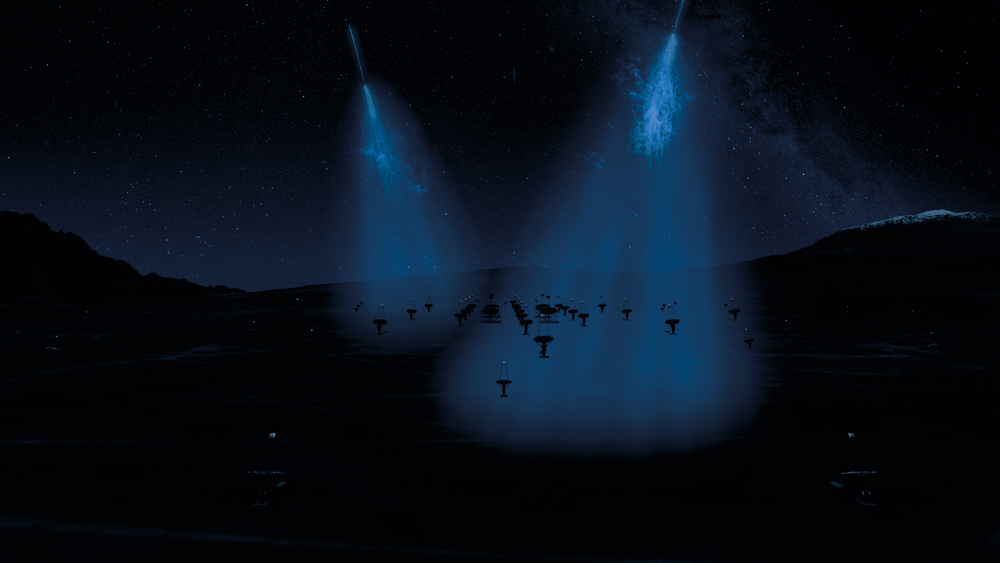
\includegraphics[trim=16cm 0 3cm 0,clip,width=\textwidth]
                        {pics/CTA_array_at_night_withtwoshower_small}};

                    \begin{scope}
                    \clip ([xshift=.5cm,yshift=1.25cm]show.south east)
                        ++(90:1.5) arc (90:-45:1.5) -- ++(-1.06cm,0);

                    \node[anchor=south west] (img) at
                        ([xshift=0cm,yshift=.5cm]show.south east)
                        {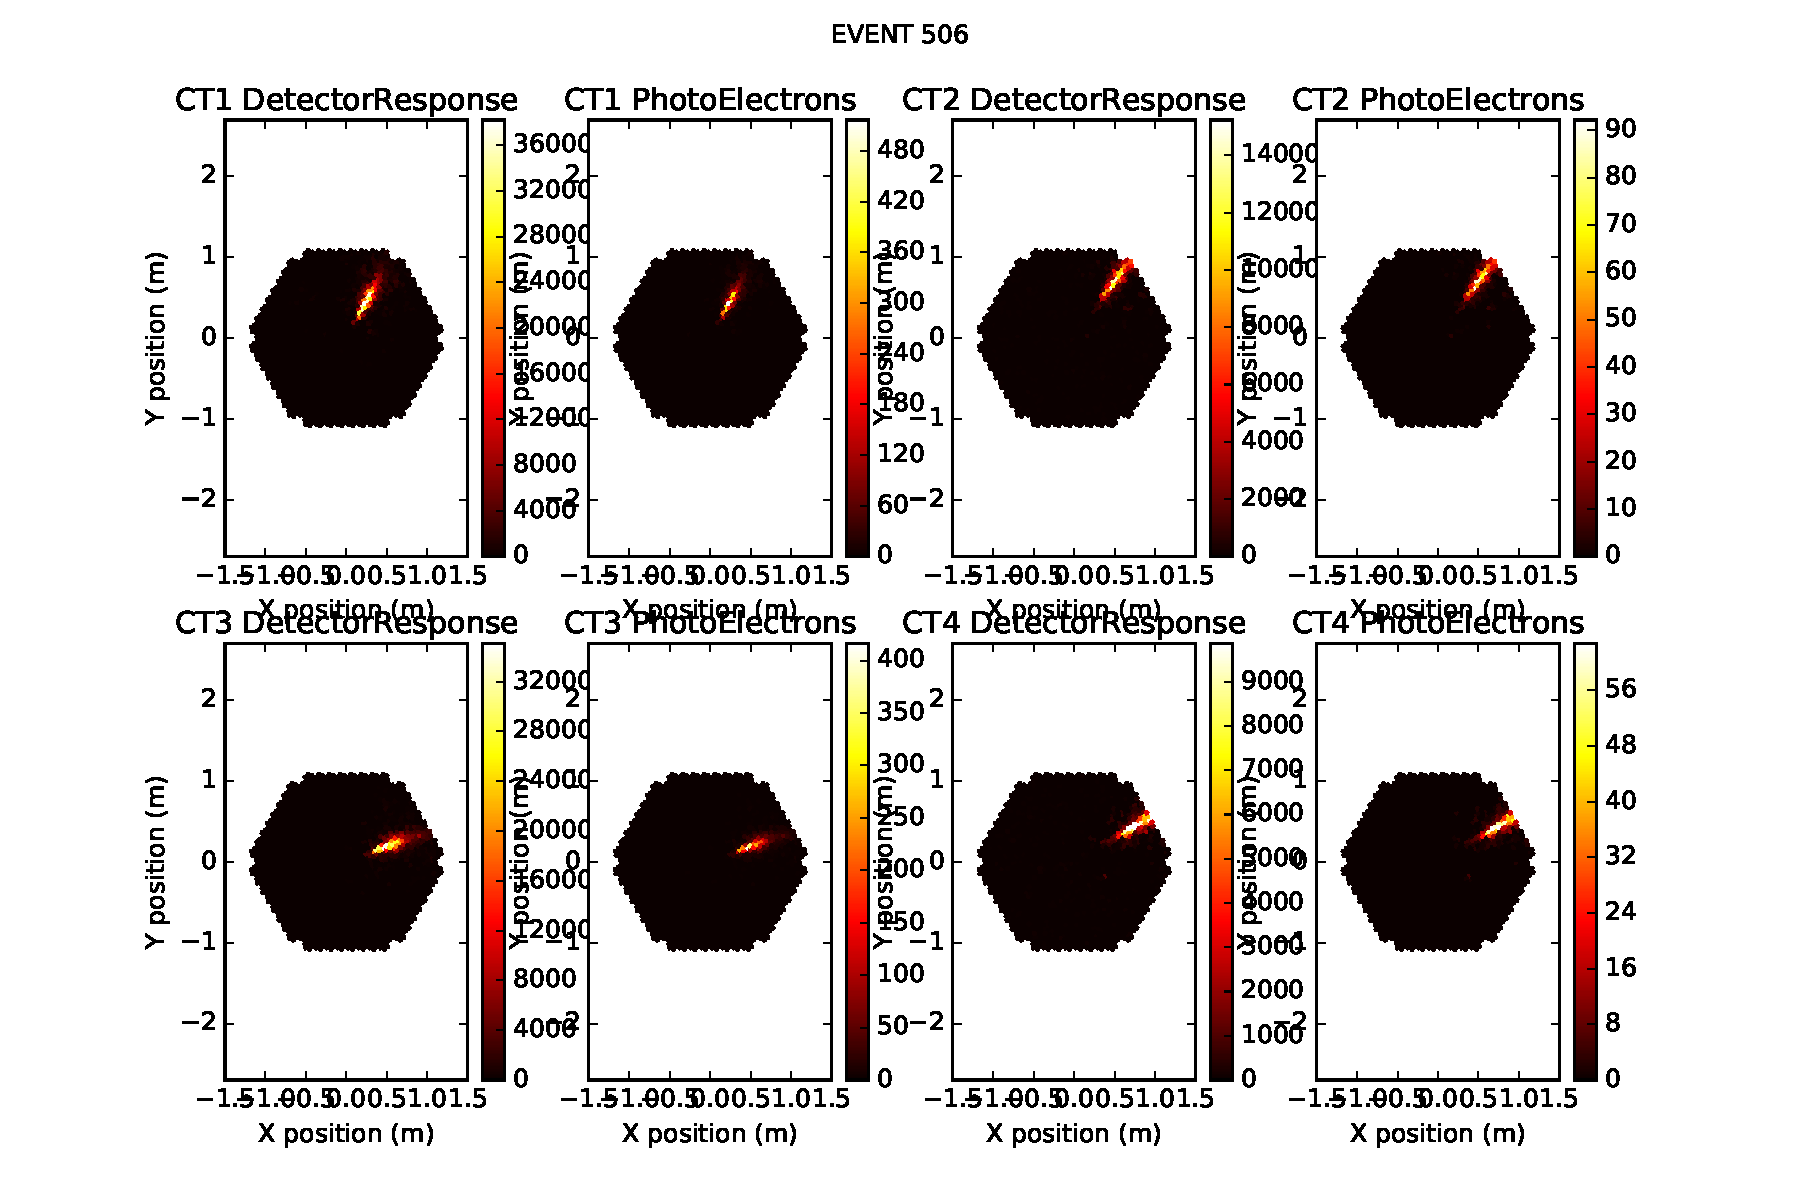
\includegraphics[trim=5.5cm 5cm 22.8cm 13cm, clip, width=2cm]
                        {pics/display.pdf}};
                    \end{scope}
                    \coordinate (shmax) at ([xshift=1cm,yshift=1cm]img.south west);
                    \foreach \P in {(shmax)}{\draw[mark options={color=blue!100!black},
                    mark size=2.402402pt,very thick,mark=star] plot coordinates {\P}
                    node[color=blue!50!white,shift=(120:.2)] {$c$};}

                    \coordinate (shmax_sky) at ([xshift=.275cm,yshift=-1.1cm]show.north);
                    \foreach \P in {(shmax_sky)}{\draw[mark options={color=blue!100!black},
                    mark size=2.402402pt,very thick,mark=star] plot coordinates {\P};}
%                     node[color=blue!50!white,shift=(30:.3)] {$c'$};}

                    \draw[dashed,shorten >=-.75cm,lightgray,-stealth]
                        (shmax) -- (shmax_sky);
                \end{tikzpicture}
            \column{.45\textwidth}
                \begin{itemize}
                    \item project the core position of the Hillas ellipsis
                        (vector $\vec c$ from direction reco) as a line into the sky
                    \item find the point that minimises the average distance to
                        lines from all telescopes
                    \item no unambiguous normal parametrisation of a line in $\mathbb{R}^3$
                        \frownie
                    \item need to use numeric minimiser after all
                \end{itemize}

        \end{columns}
    \end{frame}



    \begin{frame}{Shower Reconstruction -- Shower Energy}
                 {Machine learning}
        \begin{itemize}
            \item train 1 Random Decision Forest for each telescope type
            \item follow a telescope-by-telescope approach
            \item training features include: Hillas length/width/higher moments,
                number of telescopes (per size), signal on telescope,
                summed signal on all triggered telescopes, distance between telescope,
                shower impact, error estimators, ...
            \medskip
            \item then, for a given shower event, let the Forest estimate the energy from
                every telescope separately and combine them into a single energy
                estimator
        \end{itemize}
        \setlength{\figureheight}{4.5cm}
        \setlength{\figurewidth}{4.5cm}
%         % This file was created by matplotlib2tikz v0.6.13.
\begin{tikzpicture}

\begin{groupplot}[group style={group size=3 by 1}]
\nextgroupplot[
title={gamma},
xlabel={$E_\mathrm{reco}$ / TeV},
ylabel={$(E_\mathrm{reco} - E_\mathrm{MC})$ / TeV},
xmin=0.01, xmax=316.227766016838,
ymin=-1, ymax=1,
xmode=log,
width=\figurewidth,
height=\figureheight,
tick align=outside,
tick pos=left,
xmajorgrids,
x grid style={lightgray!92.026143790849673!black},
ymajorgrids,
y grid style={lightgray!92.026143790849673!black}
]
\addplot graphics [includegraphics cmd=\pgfimage,xmin=0.01, xmax=316.227766016838, ymin=-1, ymax=1] {\detokenize{pics/DeltaE_vs_recoE_wavelets_img000.png}};
\addplot [semithick, green!39.215686274509807!black, forget plot]
table {%
0.01 0
316.227766016838 0
};
\nextgroupplot[
title={proton},
xlabel={$E_\mathrm{reco}$ / TeV},
xmin=0.01, xmax=316.227766016838,
ymin=-1, ymax=1,
xmode=log,
width=\figurewidth,
height=\figureheight,
tick align=outside,
tick pos=left,
xmajorgrids,
x grid style={lightgray!92.026143790849673!black},
ymajorgrids,
y grid style={lightgray!92.026143790849673!black}
]
\addplot graphics [includegraphics cmd=\pgfimage,xmin=0.01, xmax=316.227766016838, ymin=-1, ymax=1] {\detokenize{pics/DeltaE_vs_recoE_wavelets_img001.png}};
\addplot [semithick, green!39.215686274509807!black, forget plot]
table {%
0.01 0
316.227766016838 0
};
\nextgroupplot[
title={electron},
xlabel={$E_\mathrm{reco}$ / TeV},
xmin=0.01, xmax=316.227766016838,
ymin=-1, ymax=1,
xmode=log,
width=\figurewidth,
height=\figureheight,
tick align=outside,
tick pos=left,
xmajorgrids,
x grid style={lightgray!92.026143790849673!black},
ymajorgrids,
y grid style={lightgray!92.026143790849673!black}
]
\addplot graphics [includegraphics cmd=\pgfimage,xmin=0.01, xmax=316.227766016838, ymin=-1, ymax=1] {\detokenize{pics/DeltaE_vs_recoE_wavelets_img002.png}};
\addplot [semithick, green!39.215686274509807!black, forget plot]
table {%
0.01 0
316.227766016838 0
};
\end{groupplot}

\end{tikzpicture}

        % This file was created by matplotlib2tikz v0.6.13.
\begin{tikzpicture}

\begin{groupplot}[group style={group size=3 by 1}]
\nextgroupplot[
title={gamma},
xlabel={$E_\mathrm{reco}$ / TeV},
ylabel={$E_\mathrm{MC}$ / TeV},
xmin=0.01, xmax=316.227766016838,
ymin=0.01, ymax=316.227766016838,
xmode=log,
ymode=log,
width=\figurewidth,
height=\figureheight,
tick align=outside,
tick pos=left,
xmajorgrids,
x grid style={lightgray!92.026143790849673!black},
ymajorgrids,
y grid style={lightgray!92.026143790849673!black}
]
\addplot graphics [includegraphics cmd=\pgfimage,xmin=0.01, xmax=316.227766016838, ymin=0.01, ymax=316.227766016838] {\detokenize{pics/energy_migration_wavelets_img000.png}};
\addplot [semithick, green!39.215686274509807!black, forget plot]
table {%
0.01 0.01
316.227766016838 316.227766016838
};
\nextgroupplot[
title={proton},
xlabel={$E_\mathrm{reco}$ / TeV},
xmin=0.01, xmax=316.227766016838,
ymin=0.01, ymax=316.227766016838,
xmode=log,
ymode=log,
width=\figurewidth,
height=\figureheight,
tick align=outside,
tick pos=left,
xmajorgrids,
x grid style={lightgray!92.026143790849673!black},
ymajorgrids,
y grid style={lightgray!92.026143790849673!black}
]
\addplot graphics [includegraphics cmd=\pgfimage,xmin=0.01, xmax=316.227766016838, ymin=0.01, ymax=316.227766016838] {\detokenize{pics/energy_migration_wavelets_img001.png}};
\addplot [semithick, green!39.215686274509807!black, forget plot]
table {%
0.01 0.01
316.227766016838 316.227766016838
};
\nextgroupplot[
title={electron},
xlabel={$E_\mathrm{reco}$ / TeV},
xmin=0.01, xmax=316.227766016838,
ymin=0.01, ymax=316.227766016838,
xmode=log,
ymode=log,
width=\figurewidth,
height=\figureheight,
tick align=outside,
tick pos=left,
xmajorgrids,
x grid style={lightgray!92.026143790849673!black},
ymajorgrids,
y grid style={lightgray!92.026143790849673!black}
]
\addplot graphics [includegraphics cmd=\pgfimage,xmin=0.01, xmax=316.227766016838, ymin=0.01, ymax=316.227766016838] {\detokenize{pics/energy_migration_wavelets_img002.png}};
\addplot [semithick, green!39.215686274509807!black, forget plot]
table {%
0.01 0.01
316.227766016838 316.227766016838
};
\end{groupplot}


\end{tikzpicture}

    \end{frame}


    \begin{frame}{Next Stop: Event Classification}
        \begin{columns}
                \column{.45\textwidth}

        \begin{itemize}
            \item Protons pose major background
            \item Event rate about $10^5$ times above Photons
            \item Training Random Forest Classifier
            \item (virtually identical to energy estimation)
        \end{itemize}
            \column{.575\textwidth}
        \setlength{\figureheight}{7cm}
        \setlength{\figurewidth}{\textwidth}
%         % This file was created by matplotlib2tikz v0.6.13.
\begin{tikzpicture}

\begin{groupplot}[group style={group size=3 by 1}]
\nextgroupplot[
title={gammas},
xlabel={$E_\mathrm{reco}$ / TeV},
ylabel={gammaness},
xmin=-2, xmax=2.5,
ymin=0, ymax=1,
width=\figurewidth,
height=\figureheight,
tick align=outside,
tick pos=left,
x grid style={lightgray!92.026143790849673!black},
y grid style={lightgray!92.026143790849673!black}
]
\addplot graphics [includegraphics cmd=\pgfimage,xmin=-2, xmax=2.5, ymin=0, ymax=1] {\detokenize{pics/gammaness_vs_e_reco_wavelets7.png}};
\nextgroupplot[
title={protons},
xlabel={$E_\mathrm{reco}$ / TeV},
xmin=-2, xmax=2.5,
ymin=0, ymax=1,
width=\figurewidth,
height=\figureheight,
tick align=outside,
tick pos=left,
x grid style={lightgray!92.026143790849673!black},
y grid style={lightgray!92.026143790849673!black}
]
\addplot graphics [includegraphics cmd=\pgfimage,xmin=-2, xmax=2.5, ymin=0, ymax=1] {\detokenize{pics/gammaness_vs_e_reco_wavelets8.png}};
\nextgroupplot[
title={electrons},
xlabel={$E_\mathrm{reco}$ / TeV},
xmin=-2, xmax=2.5,
ymin=0, ymax=1,
width=\figurewidth,
height=\figureheight,
tick align=outside,
tick pos=left,
x grid style={lightgray!92.026143790849673!black},
y grid style={lightgray!92.026143790849673!black},
colorbar,
colormap/viridis,
point meta min=0,
point meta max=1,
colorbar style={ytick={0,0.2,0.4,0.6,0.8,1},yticklabels={0.0,0.2,0.4,0.6,0.8,1.0},ylabel={sqrt(event fraction per E-column)}}
]
\addplot graphics [includegraphics cmd=\pgfimage,xmin=-2, xmax=2.5, ymin=0, ymax=1] {\detokenize{pics/gammaness_vs_e_reco_wavelets9.png}};
\end{groupplot}

\end{tikzpicture}

%         % This file was created by matplotlib2tikz v0.6.13.
\begin{tikzpicture}

\definecolor{color0}{rgb}{1,0.647058823529412,0}

\begin{axis}[
xlabel={gammaness},
ylabel={normalised Events},
xmin=-0.05, xmax=1.05,
ymin=0, ymax=37.480405349055,
width=\figurewidth,
height=\figureheight,
tick align=outside,
tick pos=left,
x grid style={lightgray!92.026143790849673!black},
y grid style={lightgray!92.026143790849673!black},
legend entries={{integral normalised},{gamma--wavelets},{proton--wavelets},
{electron--wavelets}},
legend style={at={(0.03,0.97)}, anchor=north west, draw=white!80.0!black},
legend cell align={left}
]
\addlegendimage{empty legend}
\addlegendimage{ybar,ybar legend,fill=color0,draw opacity=0,fill opacity=0.5};
\draw[fill=color0,draw opacity=0,fill opacity=0.5] (axis cs:0,0) rectangle (axis cs:0.01,0.126140314861623);
\draw[fill=color0,draw opacity=0,fill opacity=0.5] (axis cs:0.01,0) rectangle (axis cs:0.02,0.109059649212846);
\draw[fill=color0,draw opacity=0,fill opacity=0.5] (axis cs:0.02,0) rectangle (axis cs:0.03,0.111946522280245);
\draw[fill=color0,draw opacity=0,fill opacity=0.5] (axis cs:0.03,0) rectangle (axis cs:0.04,0.109540794724079);
\draw[fill=color0,draw opacity=0,fill opacity=0.5] (axis cs:0.04,0) rectangle (axis cs:0.05,0.114913586266183);
\draw[fill=color0,draw opacity=0,fill opacity=0.5] (axis cs:0.05,0) rectangle (axis cs:0.06,0.12349401454984);
\draw[fill=color0,draw opacity=0,fill opacity=0.5] (axis cs:0.06,0) rectangle (axis cs:0.07,0.120045805052669);
\draw[fill=color0,draw opacity=0,fill opacity=0.5] (axis cs:0.07,0) rectangle (axis cs:0.08,0.138008570805374);
\draw[fill=color0,draw opacity=0,fill opacity=0.5] (axis cs:0.08,0) rectangle (axis cs:0.09,0.131513106403726);
\draw[fill=color0,draw opacity=0,fill opacity=0.5] (axis cs:0.09,0) rectangle (axis cs:0.1,0.137286852538523);
\draw[fill=color0,draw opacity=0,fill opacity=0.5] (axis cs:0.1,0) rectangle (axis cs:0.11,0.161584700855798);
\draw[fill=color0,draw opacity=0,fill opacity=0.5] (axis cs:0.11,0) rectangle (axis cs:0.12,0.164471573923197);
\draw[fill=color0,draw opacity=0,fill opacity=0.5] (axis cs:0.12,0) rectangle (axis cs:0.13,0.154207136350222);
\draw[fill=color0,draw opacity=0,fill opacity=0.5] (axis cs:0.13,0) rectangle (axis cs:0.14,0.177061548133797);
\draw[fill=color0,draw opacity=0,fill opacity=0.5] (axis cs:0.14,0) rectangle (axis cs:0.15,0.185160830906222);
\draw[fill=color0,draw opacity=0,fill opacity=0.5] (axis cs:0.15,0) rectangle (axis cs:0.16,0.161825273611414);
\draw[fill=color0,draw opacity=0,fill opacity=0.5] (axis cs:0.16,0) rectangle (axis cs:0.17,0.195345077560656);
\draw[fill=color0,draw opacity=0,fill opacity=0.5] (axis cs:0.17,0) rectangle (axis cs:0.18,0.171849138428772);
\draw[fill=color0,draw opacity=0,fill opacity=0.5] (axis cs:0.18,0) rectangle (axis cs:0.19,0.187967513055081);
\draw[fill=color0,draw opacity=0,fill opacity=0.5] (axis cs:0.19,0) rectangle (axis cs:0.2,0.198151759709516);
\draw[fill=color0,draw opacity=0,fill opacity=0.5] (axis cs:0.2,0) rectangle (axis cs:0.21,0.17617944802987);
\draw[fill=color0,draw opacity=0,fill opacity=0.5] (axis cs:0.21,0) rectangle (axis cs:0.22,0.193741259189879);
\draw[fill=color0,draw opacity=0,fill opacity=0.5] (axis cs:0.22,0) rectangle (axis cs:0.23,0.180028612119734);
\draw[fill=color0,draw opacity=0,fill opacity=0.5] (axis cs:0.23,0) rectangle (axis cs:0.24,0.217237198321765);
\draw[fill=color0,draw opacity=0,fill opacity=0.5] (axis cs:0.24,0) rectangle (axis cs:0.25,0.187726940299465);
\draw[fill=color0,draw opacity=0,fill opacity=0.5] (axis cs:0.25,0) rectangle (axis cs:0.26,0.195345077560656);
\draw[fill=color0,draw opacity=0,fill opacity=0.5] (axis cs:0.26,0) rectangle (axis cs:0.27,0.182354148757361);
\draw[fill=color0,draw opacity=0,fill opacity=0.5] (axis cs:0.27,0) rectangle (axis cs:0.28,0.225577053849805);
\draw[fill=color0,draw opacity=0,fill opacity=0.5] (axis cs:0.28,0) rectangle (axis cs:0.29,0.202722642066233);
\draw[fill=color0,draw opacity=0,fill opacity=0.5] (axis cs:0.29,0) rectangle (axis cs:0.3,0.212666315965049);
\draw[fill=color0,draw opacity=0,fill opacity=0.5] (axis cs:0.3,0) rectangle (axis cs:0.31,0.197109277768511);
\draw[fill=color0,draw opacity=0,fill opacity=0.5] (axis cs:0.31,0) rectangle (axis cs:0.32,0.233355572948074);
\draw[fill=color0,draw opacity=0,fill opacity=0.5] (axis cs:0.32,0) rectangle (axis cs:0.33,0.214350325254365);
\draw[fill=color0,draw opacity=0,fill opacity=0.5] (axis cs:0.33,0) rectangle (axis cs:0.34,0.219963689552085);
\draw[fill=color0,draw opacity=0,fill opacity=0.5] (axis cs:0.34,0) rectangle (axis cs:0.35,0.223411899049256);
\draw[fill=color0,draw opacity=0,fill opacity=0.5] (axis cs:0.35,0) rectangle (axis cs:0.36,0.212345552290896);
\draw[fill=color0,draw opacity=0,fill opacity=0.5] (axis cs:0.36,0) rectangle (axis cs:0.37,0.272087786602342);
\draw[fill=color0,draw opacity=0,fill opacity=0.5] (axis cs:0.37,0) rectangle (axis cs:0.38,0.243058674091276);
\draw[fill=color0,draw opacity=0,fill opacity=0.5] (axis cs:0.38,0) rectangle (axis cs:0.39,0.250917384108084);
\draw[fill=color0,draw opacity=0,fill opacity=0.5] (axis cs:0.39,0) rectangle (axis cs:0.4,0.242497337661504);
\draw[fill=color0,draw opacity=0,fill opacity=0.5] (axis cs:0.4,0) rectangle (axis cs:0.41,0.302480144728569);
\draw[fill=color0,draw opacity=0,fill opacity=0.5] (axis cs:0.41,0) rectangle (axis cs:0.42,0.283956042546096);
\draw[fill=color0,draw opacity=0,fill opacity=0.5] (axis cs:0.42,0) rectangle (axis cs:0.43,0.283555087953399);
\draw[fill=color0,draw opacity=0,fill opacity=0.5] (axis cs:0.43,0) rectangle (axis cs:0.44,0.290130743273585);
\draw[fill=color0,draw opacity=0,fill opacity=0.5] (axis cs:0.44,0) rectangle (axis cs:0.45,0.290371316029202);
\draw[fill=color0,draw opacity=0,fill opacity=0.5] (axis cs:0.45,0) rectangle (axis cs:0.46,0.358453405868692);
\draw[fill=color0,draw opacity=0,fill opacity=0.5] (axis cs:0.46,0) rectangle (axis cs:0.47,0.324292074571138);
\draw[fill=color0,draw opacity=0,fill opacity=0.5] (axis cs:0.47,0) rectangle (axis cs:0.48,0.336320712351971);
\draw[fill=color0,draw opacity=0,fill opacity=0.5] (axis cs:0.48,0) rectangle (axis cs:0.49,0.333834793877262);
\draw[fill=color0,draw opacity=0,fill opacity=0.5] (axis cs:0.49,0) rectangle (axis cs:0.5,0.327178947638537);
\draw[fill=color0,draw opacity=0,fill opacity=0.5] (axis cs:0.5,0) rectangle (axis cs:0.51,0.429502559694119);
\draw[fill=color0,draw opacity=0,fill opacity=0.5] (axis cs:0.51,0) rectangle (axis cs:0.52,0.380586099385416);
\draw[fill=color0,draw opacity=0,fill opacity=0.5] (axis cs:0.52,0) rectangle (axis cs:0.53,0.386199463683136);
\draw[fill=color0,draw opacity=0,fill opacity=0.5] (axis cs:0.53,0) rectangle (axis cs:0.54,0.392775119003322);
\draw[fill=color0,draw opacity=0,fill opacity=0.5] (axis cs:0.54,0) rectangle (axis cs:0.55,0.46663095497761);
\draw[fill=color0,draw opacity=0,fill opacity=0.5] (axis cs:0.55,0) rectangle (axis cs:0.56,0.42380900447786);
\draw[fill=color0,draw opacity=0,fill opacity=0.5] (axis cs:0.56,0) rectangle (axis cs:0.57,0.442974634008647);
\draw[fill=color0,draw opacity=0,fill opacity=0.5] (axis cs:0.57,0) rectangle (axis cs:0.58,0.438644324407558);
\draw[fill=color0,draw opacity=0,fill opacity=0.5] (axis cs:0.58,0) rectangle (axis cs:0.59,0.43575745134015);
\draw[fill=color0,draw opacity=0,fill opacity=0.5] (axis cs:0.59,0) rectangle (axis cs:0.6,0.541930227485597);
\draw[fill=color0,draw opacity=0,fill opacity=0.5] (axis cs:0.6,0) rectangle (axis cs:0.61,0.500070568008313);
\draw[fill=color0,draw opacity=0,fill opacity=0.5] (axis cs:0.61,0) rectangle (axis cs:0.62,0.503518777505484);
\draw[fill=color0,draw opacity=0,fill opacity=0.5] (axis cs:0.62,0) rectangle (axis cs:0.63,0.507047177921194);
\draw[fill=color0,draw opacity=0,fill opacity=0.5] (axis cs:0.63,0) rectangle (axis cs:0.64,0.593492988106082);
\draw[fill=color0,draw opacity=0,fill opacity=0.5] (axis cs:0.64,0) rectangle (axis cs:0.65,0.526453380207597);
\draw[fill=color0,draw opacity=0,fill opacity=0.5] (axis cs:0.65,0) rectangle (axis cs:0.66,0.566308266721409);
\draw[fill=color0,draw opacity=0,fill opacity=0.5] (axis cs:0.66,0) rectangle (axis cs:0.67,0.580582250221326);
\draw[fill=color0,draw opacity=0,fill opacity=0.5] (axis cs:0.67,0) rectangle (axis cs:0.68,0.568072466929264);
\draw[fill=color0,draw opacity=0,fill opacity=0.5] (axis cs:0.68,0) rectangle (axis cs:0.69,0.693491063524037);
\draw[fill=color0,draw opacity=0,fill opacity=0.5] (axis cs:0.69,0) rectangle (axis cs:0.7,0.6189135092829);
\draw[fill=color0,draw opacity=0,fill opacity=0.5] (axis cs:0.7,0) rectangle (axis cs:0.71,0.653155031499006);
\draw[fill=color0,draw opacity=0,fill opacity=0.5] (axis cs:0.71,0) rectangle (axis cs:0.72,0.636074365850215);
\draw[fill=color0,draw opacity=0,fill opacity=0.5] (axis cs:0.72,0) rectangle (axis cs:0.73,0.752671961405713);
\draw[fill=color0,draw opacity=0,fill opacity=0.5] (axis cs:0.73,0) rectangle (axis cs:0.74,0.692528772501571);
\draw[fill=color0,draw opacity=0,fill opacity=0.5] (axis cs:0.74,0) rectangle (axis cs:0.75,0.723642848894647);
\draw[fill=color0,draw opacity=0,fill opacity=0.5] (axis cs:0.75,0) rectangle (axis cs:0.76,0.725888194613735);
\draw[fill=color0,draw opacity=0,fill opacity=0.5] (axis cs:0.76,0) rectangle (axis cs:0.77,0.848500109059648);
\draw[fill=color0,draw opacity=0,fill opacity=0.5] (axis cs:0.77,0) rectangle (axis cs:0.78,0.793890093534686);
\draw[fill=color0,draw opacity=0,fill opacity=0.5] (axis cs:0.78,0) rectangle (axis cs:0.79,0.847457627118643);
\draw[fill=color0,draw opacity=0,fill opacity=0.5] (axis cs:0.79,0) rectangle (axis cs:0.8,0.823159778801369);
\draw[fill=color0,draw opacity=0,fill opacity=0.5] (axis cs:0.8,0) rectangle (axis cs:0.81,0.961248540525281);
\draw[fill=color0,draw opacity=0,fill opacity=0.5] (axis cs:0.81,0) rectangle (axis cs:0.82,0.944248065795043);
\draw[fill=color0,draw opacity=0,fill opacity=0.5] (axis cs:0.82,0) rectangle (axis cs:0.83,0.971031832587022);
\draw[fill=color0,draw opacity=0,fill opacity=0.5] (axis cs:0.83,0) rectangle (axis cs:0.84,1.11409243126037);
\draw[fill=color0,draw opacity=0,fill opacity=0.5] (axis cs:0.84,0) rectangle (axis cs:0.85,1.05988337032808);
\draw[fill=color0,draw opacity=0,fill opacity=0.5] (axis cs:0.85,0) rectangle (axis cs:0.86,1.16886282862238);
\draw[fill=color0,draw opacity=0,fill opacity=0.5] (axis cs:0.86,0) rectangle (axis cs:0.87,1.30462605370867);
\draw[fill=color0,draw opacity=0,fill opacity=0.5] (axis cs:0.87,0) rectangle (axis cs:0.88,1.2209067347541);
\draw[fill=color0,draw opacity=0,fill opacity=0.5] (axis cs:0.88,0) rectangle (axis cs:0.89,1.37864227152003);
\draw[fill=color0,draw opacity=0,fill opacity=0.5] (axis cs:0.89,0) rectangle (axis cs:0.9,1.52659451622422);
\draw[fill=color0,draw opacity=0,fill opacity=0.5] (axis cs:0.9,0) rectangle (axis cs:0.91,1.52330668856413);
\draw[fill=color0,draw opacity=0,fill opacity=0.5] (axis cs:0.91,0) rectangle (axis cs:0.92,1.61071478977149);
\draw[fill=color0,draw opacity=0,fill opacity=0.5] (axis cs:0.92,0) rectangle (axis cs:0.93,1.82835294268594);
\draw[fill=color0,draw opacity=0,fill opacity=0.5] (axis cs:0.93,0) rectangle (axis cs:0.94,1.97117296860365);
\draw[fill=color0,draw opacity=0,fill opacity=0.5] (axis cs:0.94,0) rectangle (axis cs:0.95,2.24085502764982);
\draw[fill=color0,draw opacity=0,fill opacity=0.5] (axis cs:0.95,0) rectangle (axis cs:0.96,2.56121774721262);
\draw[fill=color0,draw opacity=0,fill opacity=0.5] (axis cs:0.96,0) rectangle (axis cs:0.97,2.93763391883396);
\draw[fill=color0,draw opacity=0,fill opacity=0.5] (axis cs:0.97,0) rectangle (axis cs:0.98,3.9016891415081);
\draw[fill=color0,draw opacity=0,fill opacity=0.5] (axis cs:0.98,0) rectangle (axis cs:0.99,6.19274368416325);
\draw[fill=color0,draw opacity=0,fill opacity=0.5] (axis cs:0.99,0) rectangle (axis cs:1,35.6956241419571);
\addlegendimage{ybar,ybar legend,fill=blue,draw opacity=0,fill opacity=0.5};
\draw[fill=blue,draw opacity=0,fill opacity=0.5] (axis cs:0,0) rectangle (axis cs:0.01,8.97831506407033);
\draw[fill=blue,draw opacity=0,fill opacity=0.5] (axis cs:0.01,0) rectangle (axis cs:0.02,5.2828251284847);
\draw[fill=blue,draw opacity=0,fill opacity=0.5] (axis cs:0.02,0) rectangle (axis cs:0.03,4.67626089672);
\draw[fill=blue,draw opacity=0,fill opacity=0.5] (axis cs:0.03,0) rectangle (axis cs:0.04,3.6676140924737);
\draw[fill=blue,draw opacity=0,fill opacity=0.5] (axis cs:0.04,0) rectangle (axis cs:0.05,3.53811492257396);
\draw[fill=blue,draw opacity=0,fill opacity=0.5] (axis cs:0.05,0) rectangle (axis cs:0.06,3.20519266971184);
\draw[fill=blue,draw opacity=0,fill opacity=0.5] (axis cs:0.06,0) rectangle (axis cs:0.07,2.37473954611776);
\draw[fill=blue,draw opacity=0,fill opacity=0.5] (axis cs:0.07,0) rectangle (axis cs:0.08,2.58274979313655);
\draw[fill=blue,draw opacity=0,fill opacity=0.5] (axis cs:0.08,0) rectangle (axis cs:0.09,1.85956573670737);
\draw[fill=blue,draw opacity=0,fill opacity=0.5] (axis cs:0.09,0) rectangle (axis cs:0.1,1.86997507052764);
\draw[fill=blue,draw opacity=0,fill opacity=0.5] (axis cs:0.1,0) rectangle (axis cs:0.11,1.926961762459);
\draw[fill=blue,draw opacity=0,fill opacity=0.5] (axis cs:0.11,0) rectangle (axis cs:0.12,1.56792796035279);
\draw[fill=blue,draw opacity=0,fill opacity=0.5] (axis cs:0.12,0) rectangle (axis cs:0.13,1.50194336969543);
\draw[fill=blue,draw opacity=0,fill opacity=0.5] (axis cs:0.13,0) rectangle (axis cs:0.14,1.55557790327788);
\draw[fill=blue,draw opacity=0,fill opacity=0.5] (axis cs:0.14,0) rectangle (axis cs:0.15,1.29869671611983);
\draw[fill=blue,draw opacity=0,fill opacity=0.5] (axis cs:0.15,0) rectangle (axis cs:0.16,1.27964234234711);
\draw[fill=blue,draw opacity=0,fill opacity=0.5] (axis cs:0.16,0) rectangle (axis cs:0.17,1.34121619833486);
\draw[fill=blue,draw opacity=0,fill opacity=0.5] (axis cs:0.17,0) rectangle (axis cs:0.18,1.11521015386407);
\draw[fill=blue,draw opacity=0,fill opacity=0.5] (axis cs:0.18,0) rectangle (axis cs:0.19,1.07886570018648);
\draw[fill=blue,draw opacity=0,fill opacity=0.5] (axis cs:0.19,0) rectangle (axis cs:0.2,1.20607128805802);
\draw[fill=blue,draw opacity=0,fill opacity=0.5] (axis cs:0.2,0) rectangle (axis cs:0.21,0.884440515950102);
\draw[fill=blue,draw opacity=0,fill opacity=0.5] (axis cs:0.21,0) rectangle (axis cs:0.22,0.903318460336026);
\draw[fill=blue,draw opacity=0,fill opacity=0.5] (axis cs:0.22,0) rectangle (axis cs:0.23,0.876677622931584);
\draw[fill=blue,draw opacity=0,fill opacity=0.5] (axis cs:0.23,0) rectangle (axis cs:0.24,0.997002464718537);
\draw[fill=blue,draw opacity=0,fill opacity=0.5] (axis cs:0.24,0) rectangle (axis cs:0.25,0.717185457278505);
\draw[fill=blue,draw opacity=0,fill opacity=0.5] (axis cs:0.25,0) rectangle (axis cs:0.26,0.764821391710287);
\draw[fill=blue,draw opacity=0,fill opacity=0.5] (axis cs:0.26,0) rectangle (axis cs:0.27,0.71859689237278);
\draw[fill=blue,draw opacity=0,fill opacity=0.5] (axis cs:0.27,0) rectangle (axis cs:0.28,0.821808083641642);
\draw[fill=blue,draw opacity=0,fill opacity=0.5] (axis cs:0.28,0) rectangle (axis cs:0.29,0.624912887990281);
\draw[fill=blue,draw opacity=0,fill opacity=0.5] (axis cs:0.29,0) rectangle (axis cs:0.3,0.642202967895143);
\draw[fill=blue,draw opacity=0,fill opacity=0.5] (axis cs:0.3,0) rectangle (axis cs:0.31,0.621384300254587);
\draw[fill=blue,draw opacity=0,fill opacity=0.5] (axis cs:0.31,0) rectangle (axis cs:0.32,0.705893976524305);
\draw[fill=blue,draw opacity=0,fill opacity=0.5] (axis cs:0.32,0) rectangle (axis cs:0.33,0.537403912145222);
\draw[fill=blue,draw opacity=0,fill opacity=0.5] (axis cs:0.33,0) rectangle (axis cs:0.34,0.555928997757582);
\draw[fill=blue,draw opacity=0,fill opacity=0.5] (axis cs:0.34,0) rectangle (axis cs:0.35,0.541638217428047);
\draw[fill=blue,draw opacity=0,fill opacity=0.5] (axis cs:0.35,0) rectangle (axis cs:0.36,0.515526668183964);
\draw[fill=blue,draw opacity=0,fill opacity=0.5] (axis cs:0.36,0) rectangle (axis cs:0.37,0.608681384406111);
\draw[fill=blue,draw opacity=0,fill opacity=0.5] (axis cs:0.37,0) rectangle (axis cs:0.38,0.500177311533718);
\draw[fill=blue,draw opacity=0,fill opacity=0.5] (axis cs:0.38,0) rectangle (axis cs:0.39,0.494708000543402);
\draw[fill=blue,draw opacity=0,fill opacity=0.5] (axis cs:0.39,0) rectangle (axis cs:0.4,0.479005785119592);
\draw[fill=blue,draw opacity=0,fill opacity=0.5] (axis cs:0.4,0) rectangle (axis cs:0.41,0.565809043417507);
\draw[fill=blue,draw opacity=0,fill opacity=0.5] (axis cs:0.41,0) rectangle (axis cs:0.42,0.434898438423502);
\draw[fill=blue,draw opacity=0,fill opacity=0.5] (axis cs:0.42,0) rectangle (axis cs:0.43,0.467714304365392);
\draw[fill=blue,draw opacity=0,fill opacity=0.5] (axis cs:0.43,0) rectangle (axis cs:0.44,0.454305670969779);
\draw[fill=blue,draw opacity=0,fill opacity=0.5] (axis cs:0.44,0) rectangle (axis cs:0.45,0.444778484083422);
\draw[fill=blue,draw opacity=0,fill opacity=0.5] (axis cs:0.45,0) rectangle (axis cs:0.46,0.514820950636821);
\draw[fill=blue,draw opacity=0,fill opacity=0.5] (axis cs:0.46,0) rectangle (axis cs:0.47,0.424489104603218);
\draw[fill=blue,draw opacity=0,fill opacity=0.5] (axis cs:0.47,0) rectangle (axis cs:0.48,0.447248495498408);
\draw[fill=blue,draw opacity=0,fill opacity=0.5] (axis cs:0.48,0) rectangle (axis cs:0.49,0.442484902055225);
\draw[fill=blue,draw opacity=0,fill opacity=0.5] (axis cs:0.49,0) rectangle (axis cs:0.5,0.401906143094818);
\draw[fill=blue,draw opacity=0,fill opacity=0.5] (axis cs:0.5,0) rectangle (axis cs:0.51,0.508645922099368);
\draw[fill=blue,draw opacity=0,fill opacity=0.5] (axis cs:0.51,0) rectangle (axis cs:0.52,0.41972551116004);
\draw[fill=blue,draw opacity=0,fill opacity=0.5] (axis cs:0.52,0) rectangle (axis cs:0.53,0.439132743706322);
\draw[fill=blue,draw opacity=0,fill opacity=0.5] (axis cs:0.53,0) rectangle (axis cs:0.54,0.41972551116004);
\draw[fill=blue,draw opacity=0,fill opacity=0.5] (axis cs:0.54,0) rectangle (axis cs:0.55,0.488356542619164);
\draw[fill=blue,draw opacity=0,fill opacity=0.5] (axis cs:0.55,0) rectangle (axis cs:0.56,0.433839862102791);
\draw[fill=blue,draw opacity=0,fill opacity=0.5] (axis cs:0.56,0) rectangle (axis cs:0.57,0.442132043281656);
\draw[fill=blue,draw opacity=0,fill opacity=0.5] (axis cs:0.57,0) rectangle (axis cs:0.58,0.441955613894882);
\draw[fill=blue,draw opacity=0,fill opacity=0.5] (axis cs:0.58,0) rectangle (axis cs:0.59,0.413550482622587);
\draw[fill=blue,draw opacity=0,fill opacity=0.5] (axis cs:0.59,0) rectangle (axis cs:0.6,0.494002282996264);
\draw[fill=blue,draw opacity=0,fill opacity=0.5] (axis cs:0.6,0) rectangle (axis cs:0.61,0.450777083234091);
\draw[fill=blue,draw opacity=0,fill opacity=0.5] (axis cs:0.61,0) rectangle (axis cs:0.62,0.468596451299313);
\draw[fill=blue,draw opacity=0,fill opacity=0.5] (axis cs:0.62,0) rectangle (axis cs:0.63,0.447072066111619);
\draw[fill=blue,draw opacity=0,fill opacity=0.5] (axis cs:0.63,0) rectangle (axis cs:0.64,0.548166104739069);
\draw[fill=blue,draw opacity=0,fill opacity=0.5] (axis cs:0.64,0) rectangle (axis cs:0.65,0.466126439884332);
\draw[fill=blue,draw opacity=0,fill opacity=0.5] (axis cs:0.65,0) rectangle (axis cs:0.66,0.508998780872937);
\draw[fill=blue,draw opacity=0,fill opacity=0.5] (axis cs:0.66,0) rectangle (axis cs:0.67,0.50794020455223);
\draw[fill=blue,draw opacity=0,fill opacity=0.5] (axis cs:0.67,0) rectangle (axis cs:0.68,0.477065061864964);
\draw[fill=blue,draw opacity=0,fill opacity=0.5] (axis cs:0.68,0) rectangle (axis cs:0.69,0.599683485680108);
\draw[fill=blue,draw opacity=0,fill opacity=0.5] (axis cs:0.69,0) rectangle (axis cs:0.7,0.516055956344312);
\draw[fill=blue,draw opacity=0,fill opacity=0.5] (axis cs:0.7,0) rectangle (axis cs:0.71,0.555928997757594);
\draw[fill=blue,draw opacity=0,fill opacity=0.5] (axis cs:0.71,0) rectangle (axis cs:0.72,0.530876024834199);
\draw[fill=blue,draw opacity=0,fill opacity=0.5] (axis cs:0.72,0) rectangle (axis cs:0.73,0.633910786716278);
\draw[fill=blue,draw opacity=0,fill opacity=0.5] (axis cs:0.73,0) rectangle (axis cs:0.74,0.537227482758437);
\draw[fill=blue,draw opacity=0,fill opacity=0.5] (axis cs:0.74,0) rectangle (axis cs:0.75,0.603917790962933);
\draw[fill=blue,draw opacity=0,fill opacity=0.5] (axis cs:0.75,0) rectangle (axis cs:0.76,0.575689089077432);
\draw[fill=blue,draw opacity=0,fill opacity=0.5] (axis cs:0.76,0) rectangle (axis cs:0.77,0.69724893657187);
\draw[fill=blue,draw opacity=0,fill opacity=0.5] (axis cs:0.77,0) rectangle (axis cs:0.78,0.590685586954104);
\draw[fill=blue,draw opacity=0,fill opacity=0.5] (axis cs:0.78,0) rectangle (axis cs:0.79,0.655964460064325);
\draw[fill=blue,draw opacity=0,fill opacity=0.5] (axis cs:0.79,0) rectangle (axis cs:0.8,0.612386401528583);
\draw[fill=blue,draw opacity=0,fill opacity=0.5] (axis cs:0.8,0) rectangle (axis cs:0.81,0.724595491523449);
\draw[fill=blue,draw opacity=0,fill opacity=0.5] (axis cs:0.81,0) rectangle (axis cs:0.82,0.650142290300441);
\draw[fill=blue,draw opacity=0,fill opacity=0.5] (axis cs:0.82,0) rectangle (axis cs:0.83,0.646790131951537);
\draw[fill=blue,draw opacity=0,fill opacity=0.5] (axis cs:0.83,0) rectangle (axis cs:0.84,0.768173550059208);
\draw[fill=blue,draw opacity=0,fill opacity=0.5] (axis cs:0.84,0) rectangle (axis cs:0.85,0.627206470018471);
\draw[fill=blue,draw opacity=0,fill opacity=0.5] (axis cs:0.85,0) rectangle (axis cs:0.86,0.674842404450254);
\draw[fill=blue,draw opacity=0,fill opacity=0.5] (axis cs:0.86,0) rectangle (axis cs:0.87,0.752471334635381);
\draw[fill=blue,draw opacity=0,fill opacity=0.5] (axis cs:0.87,0) rectangle (axis cs:0.88,0.594567033463361);
\draw[fill=blue,draw opacity=0,fill opacity=0.5] (axis cs:0.88,0) rectangle (axis cs:0.89,0.669549522846722);
\draw[fill=blue,draw opacity=0,fill opacity=0.5] (axis cs:0.89,0) rectangle (axis cs:0.9,0.68031171544057);
\draw[fill=blue,draw opacity=0,fill opacity=0.5] (axis cs:0.9,0) rectangle (axis cs:0.91,0.60180063832152);
\draw[fill=blue,draw opacity=0,fill opacity=0.5] (axis cs:0.91,0) rectangle (axis cs:0.92,0.583804840869514);
\draw[fill=blue,draw opacity=0,fill opacity=0.5] (axis cs:0.92,0) rectangle (axis cs:0.93,0.611151395821093);
\draw[fill=blue,draw opacity=0,fill opacity=0.5] (axis cs:0.93,0) rectangle (axis cs:0.94,0.591214875114458);
\draw[fill=blue,draw opacity=0,fill opacity=0.5] (axis cs:0.94,0) rectangle (axis cs:0.95,0.577982671105629);
\draw[fill=blue,draw opacity=0,fill opacity=0.5] (axis cs:0.95,0) rectangle (axis cs:0.96,0.583628411482742);
\draw[fill=blue,draw opacity=0,fill opacity=0.5] (axis cs:0.96,0) rectangle (axis cs:0.97,0.573042648275666);
\draw[fill=blue,draw opacity=0,fill opacity=0.5] (axis cs:0.97,0) rectangle (axis cs:0.98,0.682958156242335);
\draw[fill=blue,draw opacity=0,fill opacity=0.5] (axis cs:0.98,0) rectangle (axis cs:0.99,0.87367832335625);
\draw[fill=blue,draw opacity=0,fill opacity=0.5] (axis cs:0.99,0) rectangle (axis cs:1,2.02946723618072);
\addlegendimage{ybar,ybar legend,fill=red,draw opacity=0,fill opacity=0.5};
\draw[fill=red,draw opacity=0,fill opacity=0.5] (axis cs:0,0) rectangle (axis cs:0.01,0.575932298570617);
\draw[fill=red,draw opacity=0,fill opacity=0.5] (axis cs:0.01,0) rectangle (axis cs:0.02,0.504756991831164);
\draw[fill=red,draw opacity=0,fill opacity=0.5] (axis cs:0.02,0) rectangle (axis cs:0.03,0.521081603468654);
\draw[fill=red,draw opacity=0,fill opacity=0.5] (axis cs:0.03,0) rectangle (axis cs:0.04,0.508674898624161);
\draw[fill=red,draw opacity=0,fill opacity=0.5] (axis cs:0.04,0) rectangle (axis cs:0.05,0.51128683648616);
\draw[fill=red,draw opacity=0,fill opacity=0.5] (axis cs:0.05,0) rectangle (axis cs:0.06,0.52630547919265);
\draw[fill=red,draw opacity=0,fill opacity=0.5] (axis cs:0.06,0) rectangle (axis cs:0.07,0.548506951019634);
\draw[fill=red,draw opacity=0,fill opacity=0.5] (axis cs:0.07,0) rectangle (axis cs:0.08,0.564178578191625);
\draw[fill=red,draw opacity=0,fill opacity=0.5] (axis cs:0.08,0) rectangle (axis cs:0.09,0.570708422846621);
\draw[fill=red,draw opacity=0,fill opacity=0.5] (axis cs:0.09,0) rectangle (axis cs:0.1,0.618376288828088);
\draw[fill=red,draw opacity=0,fill opacity=0.5] (axis cs:0.1,0) rectangle (axis cs:0.11,0.63274194706908);
\draw[fill=red,draw opacity=0,fill opacity=0.5] (axis cs:0.11,0) rectangle (axis cs:0.12,0.607275552914597);
\draw[fill=red,draw opacity=0,fill opacity=0.5] (axis cs:0.12,0) rectangle (axis cs:0.13,0.566790516053622);
\draw[fill=red,draw opacity=0,fill opacity=0.5] (axis cs:0.13,0) rectangle (axis cs:0.14,0.664738185878557);
\draw[fill=red,draw opacity=0,fill opacity=0.5] (axis cs:0.14,0) rectangle (axis cs:0.15,0.660820279085563);
\draw[fill=red,draw opacity=0,fill opacity=0.5] (axis cs:0.15,0) rectangle (axis cs:0.16,0.588991987880607);
\draw[fill=red,draw opacity=0,fill opacity=0.5] (axis cs:0.16,0) rectangle (axis cs:0.17,0.713712020791024);
\draw[fill=red,draw opacity=0,fill opacity=0.5] (axis cs:0.17,0) rectangle (axis cs:0.18,0.614458382035094);
\draw[fill=red,draw opacity=0,fill opacity=0.5] (axis cs:0.18,0) rectangle (axis cs:0.19,0.611846444173092);
\draw[fill=red,draw opacity=0,fill opacity=0.5] (axis cs:0.19,0) rectangle (axis cs:0.2,0.701305315946532);
\draw[fill=red,draw opacity=0,fill opacity=0.5] (axis cs:0.2,0) rectangle (axis cs:0.21,0.590950941277109);
\draw[fill=red,draw opacity=0,fill opacity=0.5] (axis cs:0.21,0) rectangle (axis cs:0.22,0.677797875188548);
\draw[fill=red,draw opacity=0,fill opacity=0.5] (axis cs:0.22,0) rectangle (axis cs:0.23,0.593562879139104);
\draw[fill=red,draw opacity=0,fill opacity=0.5] (axis cs:0.23,0) rectangle (axis cs:0.24,0.67975682858505);
\draw[fill=red,draw opacity=0,fill opacity=0.5] (axis cs:0.24,0) rectangle (axis cs:0.25,0.664085201413057);
\draw[fill=red,draw opacity=0,fill opacity=0.5] (axis cs:0.25,0) rectangle (axis cs:0.26,0.680409813050546);
\draw[fill=red,draw opacity=0,fill opacity=0.5] (axis cs:0.26,0) rectangle (axis cs:0.27,0.598786754863101);
\draw[fill=red,draw opacity=0,fill opacity=0.5] (axis cs:0.27,0) rectangle (axis cs:0.28,0.711753067394525);
\draw[fill=red,draw opacity=0,fill opacity=0.5] (axis cs:0.28,0) rectangle (axis cs:0.29,0.646454620844576);
\draw[fill=red,draw opacity=0,fill opacity=0.5] (axis cs:0.29,0) rectangle (axis cs:0.3,0.723506787773518);
\draw[fill=red,draw opacity=0,fill opacity=0.5] (axis cs:0.3,0) rectangle (axis cs:0.31,0.683021750912545);
\draw[fill=red,draw opacity=0,fill opacity=0.5] (axis cs:0.31,0) rectangle (axis cs:0.32,0.790111203254473);
\draw[fill=red,draw opacity=0,fill opacity=0.5] (axis cs:0.32,0) rectangle (axis cs:0.33,0.723506787773518);
\draw[fill=red,draw opacity=0,fill opacity=0.5] (axis cs:0.33,0) rectangle (axis cs:0.34,0.740484383876506);
\draw[fill=red,draw opacity=0,fill opacity=0.5] (axis cs:0.34,0) rectangle (axis cs:0.35,0.758767948910494);
\draw[fill=red,draw opacity=0,fill opacity=0.5] (axis cs:0.35,0) rectangle (axis cs:0.36,0.707182176136036);
\draw[fill=red,draw opacity=0,fill opacity=0.5] (axis cs:0.36,0) rectangle (axis cs:0.37,0.916790189561389);
\draw[fill=red,draw opacity=0,fill opacity=0.5] (axis cs:0.37,0) rectangle (axis cs:0.38,0.781622405202979);
\draw[fill=red,draw opacity=0,fill opacity=0.5] (axis cs:0.38,0) rectangle (axis cs:0.39,0.805129845960963);
\draw[fill=red,draw opacity=0,fill opacity=0.5] (axis cs:0.39,0) rectangle (axis cs:0.4,0.752238104255498);
\draw[fill=red,draw opacity=0,fill opacity=0.5] (axis cs:0.4,0) rectangle (axis cs:0.41,0.95923417981886);
\draw[fill=red,draw opacity=0,fill opacity=0.5] (axis cs:0.41,0) rectangle (axis cs:0.42,0.836473100304951);
\draw[fill=red,draw opacity=0,fill opacity=0.5] (axis cs:0.42,0) rectangle (axis cs:0.43,0.861286509993926);
\draw[fill=red,draw opacity=0,fill opacity=0.5] (axis cs:0.43,0) rectangle (axis cs:0.44,0.822107442063952);
\draw[fill=red,draw opacity=0,fill opacity=0.5] (axis cs:0.44,0) rectangle (axis cs:0.45,0.792723141116471);
\draw[fill=red,draw opacity=0,fill opacity=0.5] (axis cs:0.45,0) rectangle (axis cs:0.46,1.00037220114533);
\draw[fill=red,draw opacity=0,fill opacity=0.5] (axis cs:0.46,0) rectangle (axis cs:0.47,0.912872282768391);
\draw[fill=red,draw opacity=0,fill opacity=0.5] (axis cs:0.47,0) rectangle (axis cs:0.48,0.905689453647906);
\draw[fill=red,draw opacity=0,fill opacity=0.5] (axis cs:0.48,0) rectangle (axis cs:0.49,0.856715618735429);
\draw[fill=red,draw opacity=0,fill opacity=0.5] (axis cs:0.49,0) rectangle (axis cs:0.5,0.798600001305968);
\draw[fill=red,draw opacity=0,fill opacity=0.5] (axis cs:0.5,0) rectangle (axis cs:0.51,1.0434691758683);
\draw[fill=red,draw opacity=0,fill opacity=0.5] (axis cs:0.51,0) rectangle (axis cs:0.52,0.84039100709794);
\draw[fill=red,draw opacity=0,fill opacity=0.5] (axis cs:0.52,0) rectangle (axis cs:0.53,0.861939494459425);
\draw[fill=red,draw opacity=0,fill opacity=0.5] (axis cs:0.53,0) rectangle (axis cs:0.54,0.871081276976419);
\draw[fill=red,draw opacity=0,fill opacity=0.5] (axis cs:0.54,0) rectangle (axis cs:0.55,1.02583859529982);
\draw[fill=red,draw opacity=0,fill opacity=0.5] (axis cs:0.55,0) rectangle (axis cs:0.56,0.838432053701441);
\draw[fill=red,draw opacity=0,fill opacity=0.5] (axis cs:0.56,0) rectangle (axis cs:0.57,0.894588717734404);
\draw[fill=red,draw opacity=0,fill opacity=0.5] (axis cs:0.57,0) rectangle (axis cs:0.58,0.876958137165935);
\draw[fill=red,draw opacity=0,fill opacity=0.5] (axis cs:0.58,0) rectangle (axis cs:0.59,0.820801473132953);
\draw[fill=red,draw opacity=0,fill opacity=0.5] (axis cs:0.59,0) rectangle (axis cs:0.6,0.965111040008356);
\draw[fill=red,draw opacity=0,fill opacity=0.5] (axis cs:0.6,0) rectangle (axis cs:0.61,0.818842519736454);
\draw[fill=red,draw opacity=0,fill opacity=0.5] (axis cs:0.61,0) rectangle (axis cs:0.62,0.84039100709794);
\draw[fill=red,draw opacity=0,fill opacity=0.5] (axis cs:0.62,0) rectangle (axis cs:0.63,0.816230581874456);
\draw[fill=red,draw opacity=0,fill opacity=0.5] (axis cs:0.63,0) rectangle (axis cs:0.64,0.905036469182397);
\draw[fill=red,draw opacity=0,fill opacity=0.5] (axis cs:0.64,0) rectangle (axis cs:0.65,0.796641047909469);
\draw[fill=red,draw opacity=0,fill opacity=0.5] (axis cs:0.65,0) rectangle (axis cs:0.66,0.836473100304942);
\draw[fill=red,draw opacity=0,fill opacity=0.5] (axis cs:0.66,0) rectangle (axis cs:0.67,0.814924612943457);
\draw[fill=red,draw opacity=0,fill opacity=0.5] (axis cs:0.67,0) rectangle (axis cs:0.68,0.758767948910494);
\draw[fill=red,draw opacity=0,fill opacity=0.5] (axis cs:0.68,0) rectangle (axis cs:0.69,0.88414096628641);
\draw[fill=red,draw opacity=0,fill opacity=0.5] (axis cs:0.69,0) rectangle (axis cs:0.7,0.763991824634491);
\draw[fill=red,draw opacity=0,fill opacity=0.5] (axis cs:0.7,0) rectangle (axis cs:0.71,0.804476861495481);
\draw[fill=red,draw opacity=0,fill opacity=0.5] (axis cs:0.71,0) rectangle (axis cs:0.72,0.73460752368701);
\draw[fill=red,draw opacity=0,fill opacity=0.5] (axis cs:0.72,0) rectangle (axis cs:0.73,0.917443174026888);
\draw[fill=red,draw opacity=0,fill opacity=0.5] (axis cs:0.73,0) rectangle (axis cs:0.74,0.748320197462501);
\draw[fill=red,draw opacity=0,fill opacity=0.5] (axis cs:0.74,0) rectangle (axis cs:0.75,0.772480622685985);
\draw[fill=red,draw opacity=0,fill opacity=0.5] (axis cs:0.75,0) rectangle (axis cs:0.76,0.750279150859);
\draw[fill=red,draw opacity=0,fill opacity=0.5] (axis cs:0.76,0) rectangle (axis cs:0.77,0.838432053701441);
\draw[fill=red,draw opacity=0,fill opacity=0.5] (axis cs:0.77,0) rectangle (axis cs:0.78,0.76464480909999);
\draw[fill=red,draw opacity=0,fill opacity=0.5] (axis cs:0.78,0) rectangle (axis cs:0.79,0.814924612943457);
\draw[fill=red,draw opacity=0,fill opacity=0.5] (axis cs:0.79,0) rectangle (axis cs:0.8,0.765950778030989);
\draw[fill=red,draw opacity=0,fill opacity=0.5] (axis cs:0.8,0) rectangle (axis cs:0.81,0.878917090562414);
\draw[fill=red,draw opacity=0,fill opacity=0.5] (axis cs:0.81,0) rectangle (axis cs:0.82,0.814271628477957);
\draw[fill=red,draw opacity=0,fill opacity=0.5] (axis cs:0.82,0) rectangle (axis cs:0.83,0.846920851752935);
\draw[fill=red,draw opacity=0,fill opacity=0.5] (axis cs:0.83,0) rectangle (axis cs:0.84,0.953357319629386);
\draw[fill=red,draw opacity=0,fill opacity=0.5] (axis cs:0.84,0) rectangle (axis cs:0.85,0.806435814891962);
\draw[fill=red,draw opacity=0,fill opacity=0.5] (axis cs:0.85,0) rectangle (axis cs:0.86,0.924626003147384);
\draw[fill=red,draw opacity=0,fill opacity=0.5] (axis cs:0.86,0) rectangle (axis cs:0.87,0.991883403093839);
\draw[fill=red,draw opacity=0,fill opacity=0.5] (axis cs:0.87,0) rectangle (axis cs:0.88,0.948133443905368);
\draw[fill=red,draw opacity=0,fill opacity=0.5] (axis cs:0.88,0) rectangle (axis cs:0.89,0.961846117680859);
\draw[fill=red,draw opacity=0,fill opacity=0.5] (axis cs:0.89,0) rectangle (axis cs:0.9,1.07677138360878);
\draw[fill=red,draw opacity=0,fill opacity=0.5] (axis cs:0.9,0) rectangle (axis cs:0.91,1.0552228962473);
\draw[fill=red,draw opacity=0,fill opacity=0.5] (axis cs:0.91,0) rectangle (axis cs:0.92,1.17406606896822);
\draw[fill=red,draw opacity=0,fill opacity=0.5] (axis cs:0.92,0) rectangle (axis cs:0.93,1.25634211162116);
\draw[fill=red,draw opacity=0,fill opacity=0.5] (axis cs:0.93,0) rectangle (axis cs:0.94,1.32033458924012);
\draw[fill=red,draw opacity=0,fill opacity=0.5] (axis cs:0.94,0) rectangle (axis cs:0.95,1.52863663373448);
\draw[fill=red,draw opacity=0,fill opacity=0.5] (axis cs:0.95,0) rectangle (axis cs:0.96,1.62789027249045);
\draw[fill=red,draw opacity=0,fill opacity=0.5] (axis cs:0.96,0) rectangle (axis cs:0.97,2.01511006053166);
\draw[fill=red,draw opacity=0,fill opacity=0.5] (axis cs:0.97,0) rectangle (axis cs:0.98,2.62956844256675);
\draw[fill=red,draw opacity=0,fill opacity=0.5] (axis cs:0.98,0) rectangle (axis cs:0.99,4.00997760263283);
\draw[fill=red,draw opacity=0,fill opacity=0.5] (axis cs:0.99,0) rectangle (axis cs:1,14.209594953736);
\end{axis}

\node at ({$(current bounding box.south west)!0.5!(current bounding box.south east)$}|-{$(current bounding box.south west)!0.98!(current bounding box.north west)$})[
  scale=0.6,
  anchor=north,
  text=black,
  rotate=0.0
]{ 0.03 TeV to 0.1 TeV};
\end{tikzpicture}
}
        % This file was created by matplotlib2tikz v0.6.13.
\begin{tikzpicture}

\definecolor{color0}{rgb}{1,0.647058823529412,0}

\begin{axis}[
xlabel={gammaness},
ylabel={normalised Events},
xmin=0., xmax=1.0,
ymin=0.1, ymax=50,
ymode=log,
width=\figurewidth,
height=\figureheight,
tick align=outside,
tick pos=left,
x grid style={lightgray!92.026143790849673!black},
y grid style={lightgray!92.026143790849673!black},
legend entries={{\hspace{-.25cm}integral normalised},{gamma--wavelets},{proton--wavelets},
    {electron--wavelets}},
legend style={at={(0.03,0.97)}, anchor=north west, draw=white!80.0!black},
legend cell align={left}
]
\addlegendimage{empty legend}
\addlegendimage{ybar,ybar legend,fill=color0,draw opacity=0,fill opacity=0.5};
\draw[fill=color0,draw opacity=0,fill opacity=0.5] (axis cs:0,0.1) rectangle (axis cs:0.01,0.0926007053205704);
\draw[fill=color0,draw opacity=0,fill opacity=0.5] (axis cs:0.01,0.1) rectangle (axis cs:0.02,0.0744200819223271);
\draw[fill=color0,draw opacity=0,fill opacity=0.5] (axis cs:0.02,0.1) rectangle (axis cs:0.03,0.0756795829408802);
\draw[fill=color0,draw opacity=0,fill opacity=0.5] (axis cs:0.03,0.1) rectangle (axis cs:0.04,0.0751867347162289);
\draw[fill=color0,draw opacity=0,fill opacity=0.5] (axis cs:0.04,0.1) rectangle (axis cs:0.05,0.0773771712702341);
\draw[fill=color0,draw opacity=0,fill opacity=0.5] (axis cs:0.05,0.1) rectangle (axis cs:0.06,0.0817580443782447);
\draw[fill=color0,draw opacity=0,fill opacity=0.5] (axis cs:0.06,0.1) rectangle (axis cs:0.07,0.0855913083477536);
\draw[fill=color0,draw opacity=0,fill opacity=0.5] (axis cs:0.07,0.1) rectangle (axis cs:0.08,0.0872888966771079);
\draw[fill=color0,draw opacity=0,fill opacity=0.5] (axis cs:0.08,0.1) rectangle (axis cs:0.09,0.0952839900992269);
\draw[fill=color0,draw opacity=0,fill opacity=0.5] (axis cs:0.09,0.1) rectangle (axis cs:0.1,0.0933125972006219);
\draw[fill=color0,draw opacity=0,fill opacity=0.5] (axis cs:0.1,0.1) rectangle (axis cs:0.11,0.113026526186669);
\draw[fill=color0,draw opacity=0,fill opacity=0.5] (axis cs:0.11,0.1) rectangle (axis cs:0.12,0.115545528223775);
\draw[fill=color0,draw opacity=0,fill opacity=0.5] (axis cs:0.12,0.1) rectangle (axis cs:0.13,0.112478917048168);
\draw[fill=color0,draw opacity=0,fill opacity=0.5] (axis cs:0.13,0.1) rectangle (axis cs:0.14,0.125621536372199);
\draw[fill=color0,draw opacity=0,fill opacity=0.5] (axis cs:0.14,0.1) rectangle (axis cs:0.15,0.133233303397368);
\draw[fill=color0,draw opacity=0,fill opacity=0.5] (axis cs:0.15,0.1) rectangle (axis cs:0.16,0.13465708715747);
\draw[fill=color0,draw opacity=0,fill opacity=0.5] (axis cs:0.16,0.1) rectangle (axis cs:0.17,0.149387772983155);
\draw[fill=color0,draw opacity=0,fill opacity=0.5] (axis cs:0.17,0.1) rectangle (axis cs:0.18,0.149387772983156);
\draw[fill=color0,draw opacity=0,fill opacity=0.5] (axis cs:0.18,0.1) rectangle (axis cs:0.19,0.153549602435765);
\draw[fill=color0,draw opacity=0,fill opacity=0.5] (axis cs:0.19,0.1) rectangle (axis cs:0.2,0.168608853744551);
\draw[fill=color0,draw opacity=0,fill opacity=0.5] (axis cs:0.2,0.1) rectangle (axis cs:0.21,0.158094758285327);
\draw[fill=color0,draw opacity=0,fill opacity=0.5] (axis cs:0.21,0.1) rectangle (axis cs:0.22,0.169923115676954);
\draw[fill=color0,draw opacity=0,fill opacity=0.5] (axis cs:0.22,0.1) rectangle (axis cs:0.23,0.167623157295249);
\draw[fill=color0,draw opacity=0,fill opacity=0.5] (axis cs:0.23,0.1) rectangle (axis cs:0.24,0.186406150745844);
\draw[fill=color0,draw opacity=0,fill opacity=0.5] (axis cs:0.24,0.1) rectangle (axis cs:0.25,0.180272928394629);
\draw[fill=color0,draw opacity=0,fill opacity=0.5] (axis cs:0.25,0.1) rectangle (axis cs:0.26,0.183668105053337);
\draw[fill=color0,draw opacity=0,fill opacity=0.5] (axis cs:0.26,0.1) rectangle (axis cs:0.27,0.18093005936083);
\draw[fill=color0,draw opacity=0,fill opacity=0.5] (axis cs:0.27,0.1) rectangle (axis cs:0.28,0.205736753334939);
\draw[fill=color0,draw opacity=0,fill opacity=0.5] (axis cs:0.28,0.1) rectangle (axis cs:0.29,0.197358333515872);
\draw[fill=color0,draw opacity=0,fill opacity=0.5] (axis cs:0.29,0.1) rectangle (axis cs:0.3,0.198508312706722);
\draw[fill=color0,draw opacity=0,fill opacity=0.5] (axis cs:0.3,0.1) rectangle (axis cs:0.31,0.197960703568221);
\draw[fill=color0,draw opacity=0,fill opacity=0.5] (axis cs:0.31,0.1) rectangle (axis cs:0.32,0.208529559941296);
\draw[fill=color0,draw opacity=0,fill opacity=0.5] (axis cs:0.32,0.1) rectangle (axis cs:0.33,0.205681992421089);
\draw[fill=color0,draw opacity=0,fill opacity=0.5] (axis cs:0.33,0.1) rectangle (axis cs:0.34,0.2103914310122);
\draw[fill=color0,draw opacity=0,fill opacity=0.5] (axis cs:0.34,0.1) rectangle (axis cs:0.35,0.21422469498171);
\draw[fill=color0,draw opacity=0,fill opacity=0.5] (axis cs:0.35,0.1) rectangle (axis cs:0.36,0.209734300046001);
\draw[fill=color0,draw opacity=0,fill opacity=0.5] (axis cs:0.36,0.1) rectangle (axis cs:0.37,0.248669309793441);
\draw[fill=color0,draw opacity=0,fill opacity=0.5] (axis cs:0.37,0.1) rectangle (axis cs:0.38,0.234705276761658);
\draw[fill=color0,draw opacity=0,fill opacity=0.5] (axis cs:0.38,0.1) rectangle (axis cs:0.39,0.233664819398506);
\draw[fill=color0,draw opacity=0,fill opacity=0.5] (axis cs:0.39,0.1) rectangle (axis cs:0.4,0.230433925481348);
\draw[fill=color0,draw opacity=0,fill opacity=0.5] (axis cs:0.4,0.1) rectangle (axis cs:0.41,0.26082623266817);
\draw[fill=color0,draw opacity=0,fill opacity=0.5] (axis cs:0.41,0.1) rectangle (axis cs:0.42,0.245000328565485);
\draw[fill=color0,draw opacity=0,fill opacity=0.5] (axis cs:0.42,0.1) rectangle (axis cs:0.43,0.254528727575405);
\draw[fill=color0,draw opacity=0,fill opacity=0.5] (axis cs:0.43,0.1) rectangle (axis cs:0.44,0.25239305193525);
\draw[fill=color0,draw opacity=0,fill opacity=0.5] (axis cs:0.44,0.1) rectangle (axis cs:0.45,0.246095546842485);
\draw[fill=color0,draw opacity=0,fill opacity=0.5] (axis cs:0.45,0.1) rectangle (axis cs:0.46,0.29423039011675);
\draw[fill=color0,draw opacity=0,fill opacity=0.5] (axis cs:0.46,0.1) rectangle (axis cs:0.47,0.275228353010755);
\draw[fill=color0,draw opacity=0,fill opacity=0.5] (axis cs:0.47,0.1) rectangle (axis cs:0.48,0.276980702253962);
\draw[fill=color0,draw opacity=0,fill opacity=0.5] (axis cs:0.48,0.1) rectangle (axis cs:0.49,0.271121284471995);
\draw[fill=color0,draw opacity=0,fill opacity=0.5] (axis cs:0.49,0.1) rectangle (axis cs:0.5,0.271011762644295);
\draw[fill=color0,draw opacity=0,fill opacity=0.5] (axis cs:0.5,0.1) rectangle (axis cs:0.51,0.338641491249205);
\draw[fill=color0,draw opacity=0,fill opacity=0.5] (axis cs:0.51,0.1) rectangle (axis cs:0.52,0.305620660197577);
\draw[fill=color0,draw opacity=0,fill opacity=0.5] (axis cs:0.52,0.1) rectangle (axis cs:0.53,0.303265940902021);
\draw[fill=color0,draw opacity=0,fill opacity=0.5] (axis cs:0.53,0.1) rectangle (axis cs:0.54,0.306332552077629);
\draw[fill=color0,draw opacity=0,fill opacity=0.5] (axis cs:0.54,0.1) rectangle (axis cs:0.55,0.354905482662694);
\draw[fill=color0,draw opacity=0,fill opacity=0.5] (axis cs:0.55,0.1) rectangle (axis cs:0.56,0.344446148117319);
\draw[fill=color0,draw opacity=0,fill opacity=0.5] (axis cs:0.56,0.1) rectangle (axis cs:0.57,0.342639037960265);
\draw[fill=color0,draw opacity=0,fill opacity=0.5] (axis cs:0.57,0.1) rectangle (axis cs:0.58,0.347786563862185);
\draw[fill=color0,draw opacity=0,fill opacity=0.5] (axis cs:0.58,0.1) rectangle (axis cs:0.59,0.350305565899283);
\draw[fill=color0,draw opacity=0,fill opacity=0.5] (axis cs:0.59,0.1) rectangle (axis cs:0.6,0.411637789411429);
\draw[fill=color0,draw opacity=0,fill opacity=0.5] (axis cs:0.6,0.1) rectangle (axis cs:0.61,0.384038288830963);
\draw[fill=color0,draw opacity=0,fill opacity=0.5] (axis cs:0.61,0.1) rectangle (axis cs:0.62,0.389350097474426);
\draw[fill=color0,draw opacity=0,fill opacity=0.5] (axis cs:0.62,0.1) rectangle (axis cs:0.63,0.390226272096028);
\draw[fill=color0,draw opacity=0,fill opacity=0.5] (axis cs:0.63,0.1) rectangle (axis cs:0.64,0.451668017435874);
\draw[fill=color0,draw opacity=0,fill opacity=0.5] (axis cs:0.64,0.1) rectangle (axis cs:0.65,0.447122861586313);
\draw[fill=color0,draw opacity=0,fill opacity=0.5] (axis cs:0.65,0.1) rectangle (axis cs:0.66,0.435130221453135);
\draw[fill=color0,draw opacity=0,fill opacity=0.5] (axis cs:0.66,0.1) rectangle (axis cs:0.67,0.451996582918975);
\draw[fill=color0,draw opacity=0,fill opacity=0.5] (axis cs:0.67,0.1) rectangle (axis cs:0.68,0.45845837075329);
\draw[fill=color0,draw opacity=0,fill opacity=0.5] (axis cs:0.68,0.1) rectangle (axis cs:0.69,0.557520863908176);
\draw[fill=color0,draw opacity=0,fill opacity=0.5] (axis cs:0.69,0.1) rectangle (axis cs:0.7,0.52548572930585);
\draw[fill=color0,draw opacity=0,fill opacity=0.5] (axis cs:0.7,0.1) rectangle (axis cs:0.71,0.528497579567619);
\draw[fill=color0,draw opacity=0,fill opacity=0.5] (axis cs:0.71,0.1) rectangle (axis cs:0.72,0.545418701947297);
\draw[fill=color0,draw opacity=0,fill opacity=0.5] (axis cs:0.72,0.1) rectangle (axis cs:0.73,0.644590716929883);
\draw[fill=color0,draw opacity=0,fill opacity=0.5] (axis cs:0.73,0.1) rectangle (axis cs:0.74,0.618195956454121);
\draw[fill=color0,draw opacity=0,fill opacity=0.5] (axis cs:0.74,0.1) rectangle (axis cs:0.75,0.619674501128074);
\draw[fill=color0,draw opacity=0,fill opacity=0.5] (axis cs:0.75,0.1) rectangle (axis cs:0.76,0.633802816901408);
\draw[fill=color0,draw opacity=0,fill opacity=0.5] (axis cs:0.76,0.1) rectangle (axis cs:0.77,0.757452960375002);
\draw[fill=color0,draw opacity=0,fill opacity=0.5] (axis cs:0.77,0.1) rectangle (axis cs:0.78,0.739327097890608);
\draw[fill=color0,draw opacity=0,fill opacity=0.5] (axis cs:0.78,0.1) rectangle (axis cs:0.79,0.741955621755415);
\draw[fill=color0,draw opacity=0,fill opacity=0.5] (axis cs:0.79,0.1) rectangle (axis cs:0.8,0.772347928942237);
\draw[fill=color0,draw opacity=0,fill opacity=0.5] (axis cs:0.8,0.1) rectangle (axis cs:0.81,0.92069524456224);
\draw[fill=color0,draw opacity=0,fill opacity=0.5] (axis cs:0.81,0.1) rectangle (axis cs:0.82,0.875079403325081);
\draw[fill=color0,draw opacity=0,fill opacity=0.5] (axis cs:0.82,0.1) rectangle (axis cs:0.83,0.919161938974436);
\draw[fill=color0,draw opacity=0,fill opacity=0.5] (axis cs:0.83,0.1) rectangle (axis cs:0.84,1.06148555407095);
\draw[fill=color0,draw opacity=0,fill opacity=0.5] (axis cs:0.84,0.1) rectangle (axis cs:0.85,1.07386152060105);
\draw[fill=color0,draw opacity=0,fill opacity=0.5] (axis cs:0.85,0.1) rectangle (axis cs:0.86,1.0945611460364);
\draw[fill=color0,draw opacity=0,fill opacity=0.5] (axis cs:0.86,0.1) rectangle (axis cs:0.87,1.25643440737739);
\draw[fill=color0,draw opacity=0,fill opacity=0.5] (axis cs:0.87,0.1) rectangle (axis cs:0.88,1.32954022736731);
\draw[fill=color0,draw opacity=0,fill opacity=0.5] (axis cs:0.88,0.1) rectangle (axis cs:0.89,1.37006330361641);
\draw[fill=color0,draw opacity=0,fill opacity=0.5] (axis cs:0.89,0.1) rectangle (axis cs:0.9,1.58773793617068);
\draw[fill=color0,draw opacity=0,fill opacity=0.5] (axis cs:0.9,0.1) rectangle (axis cs:0.91,1.66412941099161);
\draw[fill=color0,draw opacity=0,fill opacity=0.5] (axis cs:0.91,0.1) rectangle (axis cs:0.92,1.71889032484174);
\draw[fill=color0,draw opacity=0,fill opacity=0.5] (axis cs:0.92,0.1) rectangle (axis cs:0.93,2.11147131623332);
\draw[fill=color0,draw opacity=0,fill opacity=0.5] (axis cs:0.93,0.1) rectangle (axis cs:0.94,2.14974919501456);
\draw[fill=color0,draw opacity=0,fill opacity=0.5] (axis cs:0.94,0.1) rectangle (axis cs:0.95,2.67841105732372);
\draw[fill=color0,draw opacity=0,fill opacity=0.5] (axis cs:0.95,0.1) rectangle (axis cs:0.96,2.92910652092968);
\draw[fill=color0,draw opacity=0,fill opacity=0.5] (axis cs:0.96,0.1) rectangle (axis cs:0.97,3.44353054563774);
\draw[fill=color0,draw opacity=0,fill opacity=0.5] (axis cs:0.97,0.1) rectangle (axis cs:0.98,4.45167896961864);
\draw[fill=color0,draw opacity=0,fill opacity=0.5] (axis cs:0.98,0.1) rectangle (axis cs:0.99,6.25052022868157);
\draw[fill=color0,draw opacity=0,fill opacity=0.5] (axis cs:0.99,0.1) rectangle (axis cs:1,37.7521192473659);
\addlegendimage{ybar,ybar legend,fill=blue,draw opacity=0,fill opacity=0.5};
\draw[fill=blue,draw opacity=0,fill opacity=0.5] (axis cs:0,0.1) rectangle (axis cs:0.01,19.5670421082936);
\draw[fill=blue,draw opacity=0,fill opacity=0.5] (axis cs:0.01,0.1) rectangle (axis cs:0.02,5.66376617149926);
\draw[fill=blue,draw opacity=0,fill opacity=0.5] (axis cs:0.02,0.1) rectangle (axis cs:0.03,4.18331085251571);
\draw[fill=blue,draw opacity=0,fill opacity=0.5] (axis cs:0.03,0.1) rectangle (axis cs:0.04,3.29984511167928);
\draw[fill=blue,draw opacity=0,fill opacity=0.5] (axis cs:0.04,0.1) rectangle (axis cs:0.05,2.97693547314615);
\draw[fill=blue,draw opacity=0,fill opacity=0.5] (axis cs:0.05,0.1) rectangle (axis cs:0.06,2.70609733926952);
\draw[fill=blue,draw opacity=0,fill opacity=0.5] (axis cs:0.06,0.1) rectangle (axis cs:0.07,2.2200475108734);
\draw[fill=blue,draw opacity=0,fill opacity=0.5] (axis cs:0.07,0.1) rectangle (axis cs:0.08,2.28072085234441);
\draw[fill=blue,draw opacity=0,fill opacity=0.5] (axis cs:0.08,0.1) rectangle (axis cs:0.09,1.83499098280683);
\draw[fill=blue,draw opacity=0,fill opacity=0.5] (axis cs:0.09,0.1) rectangle (axis cs:0.1,1.81233518134679);
\draw[fill=blue,draw opacity=0,fill opacity=0.5] (axis cs:0.1,0.1) rectangle (axis cs:0.11,1.78503770349008);
\draw[fill=blue,draw opacity=0,fill opacity=0.5] (axis cs:0.11,0.1) rectangle (axis cs:0.12,1.57944091007802);
\draw[fill=blue,draw opacity=0,fill opacity=0.5] (axis cs:0.12,0.1) rectangle (axis cs:0.13,1.49557760597435);
\draw[fill=blue,draw opacity=0,fill opacity=0.5] (axis cs:0.13,0.1) rectangle (axis cs:0.14,1.53055595310654);
\draw[fill=blue,draw opacity=0,fill opacity=0.5] (axis cs:0.14,0.1) rectangle (axis cs:0.15,1.34663873556315);
\draw[fill=blue,draw opacity=0,fill opacity=0.5] (axis cs:0.15,0.1) rectangle (axis cs:0.16,1.27986858898379);
\draw[fill=blue,draw opacity=0,fill opacity=0.5] (axis cs:0.16,0.1) rectangle (axis cs:0.17,1.32757470750531);
\draw[fill=blue,draw opacity=0,fill opacity=0.5] (axis cs:0.17,0.1) rectangle (axis cs:0.18,1.13827903953401);
\draw[fill=blue,draw opacity=0,fill opacity=0.5] (axis cs:0.18,0.1) rectangle (axis cs:0.19,1.11387339974983);
\draw[fill=blue,draw opacity=0,fill opacity=0.5] (axis cs:0.19,0.1) rectangle (axis cs:0.2,1.18493525506104);
\draw[fill=blue,draw opacity=0,fill opacity=0.5] (axis cs:0.2,0.1) rectangle (axis cs:0.21,0.954453918744511);
\draw[fill=blue,draw opacity=0,fill opacity=0.5] (axis cs:0.21,0.1) rectangle (axis cs:0.22,0.977220236309217);
\draw[fill=blue,draw opacity=0,fill opacity=0.5] (axis cs:0.22,0.1) rectangle (axis cs:0.23,0.936126664717898);
\draw[fill=blue,draw opacity=0,fill opacity=0.5] (axis cs:0.23,0.1) rectangle (axis cs:0.24,0.982451331930888);
\draw[fill=blue,draw opacity=0,fill opacity=0.5] (axis cs:0.24,0.1) rectangle (axis cs:0.25,0.821189915847511);
\draw[fill=blue,draw opacity=0,fill opacity=0.5] (axis cs:0.25,0.1) rectangle (axis cs:0.26,0.826089463155126);
\draw[fill=blue,draw opacity=0,fill opacity=0.5] (axis cs:0.26,0.1) rectangle (axis cs:0.27,0.805754499893442);
\draw[fill=blue,draw opacity=0,fill opacity=0.5] (axis cs:0.27,0.1) rectangle (axis cs:0.28,0.852152844509549);
\draw[fill=blue,draw opacity=0,fill opacity=0.5] (axis cs:0.28,0.1) rectangle (axis cs:0.29,0.712773617153432);
\draw[fill=blue,draw opacity=0,fill opacity=0.5] (axis cs:0.29,0.1) rectangle (axis cs:0.3,0.718630970701627);
\draw[fill=blue,draw opacity=0,fill opacity=0.5] (axis cs:0.3,0.1) rectangle (axis cs:0.31,0.702790329030387);
\draw[fill=blue,draw opacity=0,fill opacity=0.5] (axis cs:0.31,0.1) rectangle (axis cs:0.32,0.758122058775042);
\draw[fill=blue,draw opacity=0,fill opacity=0.5] (axis cs:0.32,0.1) rectangle (axis cs:0.33,0.636683279079134);
\draw[fill=blue,draw opacity=0,fill opacity=0.5] (axis cs:0.33,0.1) rectangle (axis cs:0.34,0.641288116774262);
\draw[fill=blue,draw opacity=0,fill opacity=0.5] (axis cs:0.34,0.1) rectangle (axis cs:0.35,0.624287056003851);
\draw[fill=blue,draw opacity=0,fill opacity=0.5] (axis cs:0.35,0.1) rectangle (axis cs:0.36,0.614782671001114);
\draw[fill=blue,draw opacity=0,fill opacity=0.5] (axis cs:0.36,0.1) rectangle (axis cs:0.37,0.656170952204915);
\draw[fill=blue,draw opacity=0,fill opacity=0.5] (axis cs:0.37,0.1) rectangle (axis cs:0.38,0.570981454845052);
\draw[fill=blue,draw opacity=0,fill opacity=0.5] (axis cs:0.38,0.1) rectangle (axis cs:0.39,0.577078259953402);
\draw[fill=blue,draw opacity=0,fill opacity=0.5] (axis cs:0.39,0.1) rectangle (axis cs:0.4,0.560611360355625);
\draw[fill=blue,draw opacity=0,fill opacity=0.5] (axis cs:0.4,0.1) rectangle (axis cs:0.41,0.620787379355554);
\draw[fill=blue,draw opacity=0,fill opacity=0.5] (axis cs:0.41,0.1) rectangle (axis cs:0.42,0.531490366771643);
\draw[fill=blue,draw opacity=0,fill opacity=0.5] (axis cs:0.42,0.1) rectangle (axis cs:0.43,0.52725391609212);
\draw[fill=blue,draw opacity=0,fill opacity=0.5] (axis cs:0.43,0.1) rectangle (axis cs:0.44,0.529887883253733);
\draw[fill=blue,draw opacity=0,fill opacity=0.5] (axis cs:0.44,0.1) rectangle (axis cs:0.45,0.52401211035475);
\draw[fill=blue,draw opacity=0,fill opacity=0.5] (axis cs:0.45,0.1) rectangle (axis cs:0.46,0.567850165212366);
\draw[fill=blue,draw opacity=0,fill opacity=0.5] (axis cs:0.46,0.1) rectangle (axis cs:0.47,0.497506664581595);
\draw[fill=blue,draw opacity=0,fill opacity=0.5] (axis cs:0.47,0.1) rectangle (axis cs:0.48,0.497746116141747);
\draw[fill=blue,draw opacity=0,fill opacity=0.5] (axis cs:0.48,0.1) rectangle (axis cs:0.49,0.493528084813005);
\draw[fill=blue,draw opacity=0,fill opacity=0.5] (axis cs:0.49,0.1) rectangle (axis cs:0.5,0.491870343242759);
\draw[fill=blue,draw opacity=0,fill opacity=0.5] (axis cs:0.5,0.1) rectangle (axis cs:0.51,0.528395915840512);
\draw[fill=blue,draw opacity=0,fill opacity=0.5] (axis cs:0.51,0.1) rectangle (axis cs:0.52,0.464407091229017);
\draw[fill=blue,draw opacity=0,fill opacity=0.5] (axis cs:0.52,0.1) rectangle (axis cs:0.53,0.475366604943421);
\draw[fill=blue,draw opacity=0,fill opacity=0.5] (axis cs:0.53,0.1) rectangle (axis cs:0.54,0.464296575124334);
\draw[fill=blue,draw opacity=0,fill opacity=0.5] (axis cs:0.54,0.1) rectangle (axis cs:0.55,0.519517788764306);
\draw[fill=blue,draw opacity=0,fill opacity=0.5] (axis cs:0.55,0.1) rectangle (axis cs:0.56,0.441714451067428);
\draw[fill=blue,draw opacity=0,fill opacity=0.5] (axis cs:0.56,0.1) rectangle (axis cs:0.57,0.450979384510025);
\draw[fill=blue,draw opacity=0,fill opacity=0.5] (axis cs:0.57,0.1) rectangle (axis cs:0.58,0.44176970911978);
\draw[fill=blue,draw opacity=0,fill opacity=0.5] (axis cs:0.58,0.1) rectangle (axis cs:0.59,0.440167225601865);
\draw[fill=blue,draw opacity=0,fill opacity=0.5] (axis cs:0.59,0.1) rectangle (axis cs:0.6,0.486639247621094);
\draw[fill=blue,draw opacity=0,fill opacity=0.5] (axis cs:0.6,0.1) rectangle (axis cs:0.61,0.424252906527504);
\draw[fill=blue,draw opacity=0,fill opacity=0.5] (axis cs:0.61,0.1) rectangle (axis cs:0.62,0.427863099280484);
\draw[fill=blue,draw opacity=0,fill opacity=0.5] (axis cs:0.62,0.1) rectangle (axis cs:0.63,0.427844679929704);
\draw[fill=blue,draw opacity=0,fill opacity=0.5] (axis cs:0.63,0.1) rectangle (axis cs:0.64,0.476305991833227);
\draw[fill=blue,draw opacity=0,fill opacity=0.5] (axis cs:0.64,0.1) rectangle (axis cs:0.65,0.400510363371426);
\draw[fill=blue,draw opacity=0,fill opacity=0.5] (axis cs:0.65,0.1) rectangle (axis cs:0.66,0.410696264353048);
\draw[fill=blue,draw opacity=0,fill opacity=0.5] (axis cs:0.66,0.1) rectangle (axis cs:0.67,0.409591103306217);
\draw[fill=blue,draw opacity=0,fill opacity=0.5] (axis cs:0.67,0.1) rectangle (axis cs:0.68,0.405483588082164);
\draw[fill=blue,draw opacity=0,fill opacity=0.5] (axis cs:0.68,0.1) rectangle (axis cs:0.69,0.444274740825919);
\draw[fill=blue,draw opacity=0,fill opacity=0.5] (axis cs:0.69,0.1) rectangle (axis cs:0.7,0.385848560150139);
\draw[fill=blue,draw opacity=0,fill opacity=0.5] (axis cs:0.7,0.1) rectangle (axis cs:0.71,0.392866332797522);
\draw[fill=blue,draw opacity=0,fill opacity=0.5] (axis cs:0.71,0.1) rectangle (axis cs:0.72,0.389771881866388);
\draw[fill=blue,draw opacity=0,fill opacity=0.5] (axis cs:0.72,0.1) rectangle (axis cs:0.73,0.421600520015111);
\draw[fill=blue,draw opacity=0,fill opacity=0.5] (axis cs:0.73,0.1) rectangle (axis cs:0.74,0.366747693390749);
\draw[fill=blue,draw opacity=0,fill opacity=0.5] (axis cs:0.74,0.1) rectangle (axis cs:0.75,0.373839143441246);
\draw[fill=blue,draw opacity=0,fill opacity=0.5] (axis cs:0.75,0.1) rectangle (axis cs:0.76,0.37253136953583);
\draw[fill=blue,draw opacity=0,fill opacity=0.5] (axis cs:0.76,0.1) rectangle (axis cs:0.77,0.402425975852599);
\draw[fill=blue,draw opacity=0,fill opacity=0.5] (axis cs:0.77,0.1) rectangle (axis cs:0.78,0.353154212514733);
\draw[fill=blue,draw opacity=0,fill opacity=0.5] (axis cs:0.78,0.1) rectangle (axis cs:0.79,0.361590275172206);
\draw[fill=blue,draw opacity=0,fill opacity=0.5] (axis cs:0.79,0.1) rectangle (axis cs:0.8,0.347831020139165);
\draw[fill=blue,draw opacity=0,fill opacity=0.5] (axis cs:0.8,0.1) rectangle (axis cs:0.81,0.377909819963739);
\draw[fill=blue,draw opacity=0,fill opacity=0.5] (axis cs:0.81,0.1) rectangle (axis cs:0.82,0.336447861356809);
\draw[fill=blue,draw opacity=0,fill opacity=0.5] (axis cs:0.82,0.1) rectangle (axis cs:0.83,0.342526247114378);
\draw[fill=blue,draw opacity=0,fill opacity=0.5] (axis cs:0.83,0.1) rectangle (axis cs:0.84,0.360264081916018);
\draw[fill=blue,draw opacity=0,fill opacity=0.5] (axis cs:0.84,0.1) rectangle (axis cs:0.85,0.317568026806786);
\draw[fill=blue,draw opacity=0,fill opacity=0.5] (axis cs:0.85,0.1) rectangle (axis cs:0.86,0.330958894824217);
\draw[fill=blue,draw opacity=0,fill opacity=0.5] (axis cs:0.86,0.1) rectangle (axis cs:0.87,0.353006857708488);
\draw[fill=blue,draw opacity=0,fill opacity=0.5] (axis cs:0.87,0.1) rectangle (axis cs:0.88,0.299388127586422);
\draw[fill=blue,draw opacity=0,fill opacity=0.5] (axis cs:0.88,0.1) rectangle (axis cs:0.89,0.312429027939023);
\draw[fill=blue,draw opacity=0,fill opacity=0.5] (axis cs:0.89,0.1) rectangle (axis cs:0.9,0.326980315055627);
\draw[fill=blue,draw opacity=0,fill opacity=0.5] (axis cs:0.9,0.1) rectangle (axis cs:0.91,0.298006676277883);
\draw[fill=blue,draw opacity=0,fill opacity=0.5] (axis cs:0.91,0.1) rectangle (axis cs:0.92,0.296183160550613);
\draw[fill=blue,draw opacity=0,fill opacity=0.5] (axis cs:0.92,0.1) rectangle (axis cs:0.93,0.295593741325636);
\draw[fill=blue,draw opacity=0,fill opacity=0.5] (axis cs:0.93,0.1) rectangle (axis cs:0.94,0.284873679171379);
\draw[fill=blue,draw opacity=0,fill opacity=0.5] (axis cs:0.94,0.1) rectangle (axis cs:0.95,0.284984195276062);
\draw[fill=blue,draw opacity=0,fill opacity=0.5] (axis cs:0.95,0.1) rectangle (axis cs:0.96,0.29189145181876);
\draw[fill=blue,draw opacity=0,fill opacity=0.5] (axis cs:0.96,0.1) rectangle (axis cs:0.97,0.280158325371568);
\draw[fill=blue,draw opacity=0,fill opacity=0.5] (axis cs:0.97,0.1) rectangle (axis cs:0.98,0.308855673887604);
\draw[fill=blue,draw opacity=0,fill opacity=0.5] (axis cs:0.98,0.1) rectangle (axis cs:0.99,0.358495824241081);
\draw[fill=blue,draw opacity=0,fill opacity=0.5] (axis cs:0.99,0.1) rectangle (axis cs:1,0.69674878197438);
\addlegendimage{ybar,ybar legend,fill=red,draw opacity=0,fill opacity=0.5};
\draw[fill=red,draw opacity=0,fill opacity=0.5] (axis cs:0,0.1) rectangle (axis cs:0.01,1.3939005189807);
\draw[fill=red,draw opacity=0,fill opacity=0.5] (axis cs:0.01,0.1) rectangle (axis cs:0.02,0.990145197970727);
\draw[fill=red,draw opacity=0,fill opacity=0.5] (axis cs:0.02,0.1) rectangle (axis cs:0.03,0.878418566680273);
\draw[fill=red,draw opacity=0,fill opacity=0.5] (axis cs:0.03,0.1) rectangle (axis cs:0.04,0.800046649950434);
\draw[fill=red,draw opacity=0,fill opacity=0.5] (axis cs:0.04,0.1) rectangle (axis cs:0.05,0.753863199020351);
\draw[fill=red,draw opacity=0,fill opacity=0.5] (axis cs:0.05,0.1) rectangle (axis cs:0.06,0.738935214881335);
\draw[fill=red,draw opacity=0,fill opacity=0.5] (axis cs:0.06,0.1) rectangle (axis cs:0.07,0.711411744125021);
\draw[fill=red,draw opacity=0,fill opacity=0.5] (axis cs:0.07,0.1) rectangle (axis cs:0.08,0.734969969094409);
\draw[fill=red,draw opacity=0,fill opacity=0.5] (axis cs:0.08,0.1) rectangle (axis cs:0.09,0.698816257507727);
\draw[fill=red,draw opacity=0,fill opacity=0.5] (axis cs:0.09,0.1) rectangle (axis cs:0.1,0.718175986938013);
\draw[fill=red,draw opacity=0,fill opacity=0.5] (axis cs:0.1,0.1) rectangle (axis cs:0.11,0.733103971077032);
\draw[fill=red,draw opacity=0,fill opacity=0.5] (axis cs:0.11,0.1) rectangle (axis cs:0.12,0.744766458685639);
\draw[fill=red,draw opacity=0,fill opacity=0.5] (axis cs:0.12,0.1) rectangle (axis cs:0.13,0.700682255525102);
\draw[fill=red,draw opacity=0,fill opacity=0.5] (axis cs:0.13,0.1) rectangle (axis cs:0.14,0.738701965129161);
\draw[fill=red,draw opacity=0,fill opacity=0.5] (axis cs:0.14,0.1) rectangle (axis cs:0.15,0.70441425155986);
\draw[fill=red,draw opacity=0,fill opacity=0.5] (axis cs:0.15,0.1) rectangle (axis cs:0.16,0.710012245611988);
\draw[fill=red,draw opacity=0,fill opacity=0.5] (axis cs:0.16,0.1) rectangle (axis cs:0.17,0.748731704472563);
\draw[fill=red,draw opacity=0,fill opacity=0.5] (axis cs:0.17,0.1) rectangle (axis cs:0.18,0.715143740159779);
\draw[fill=red,draw opacity=0,fill opacity=0.5] (axis cs:0.18,0.1) rectangle (axis cs:0.19,0.722374482477111);
\draw[fill=red,draw opacity=0,fill opacity=0.5] (axis cs:0.19,0.1) rectangle (axis cs:0.2,0.779054172254941);
\draw[fill=red,draw opacity=0,fill opacity=0.5] (axis cs:0.2,0.1) rectangle (axis cs:0.21,0.716309988920639);
\draw[fill=red,draw opacity=0,fill opacity=0.5] (axis cs:0.21,0.1) rectangle (axis cs:0.22,0.737302466616128);
\draw[fill=red,draw opacity=0,fill opacity=0.5] (axis cs:0.22,0.1) rectangle (axis cs:0.23,0.744299959181292);
\draw[fill=red,draw opacity=0,fill opacity=0.5] (axis cs:0.23,0.1) rectangle (axis cs:0.24,0.790250160359208);
\draw[fill=red,draw opacity=0,fill opacity=0.5] (axis cs:0.24,0.1) rectangle (axis cs:0.25,0.780920170272318);
\draw[fill=red,draw opacity=0,fill opacity=0.5] (axis cs:0.25,0.1) rectangle (axis cs:0.26,0.779287422007113);
\draw[fill=red,draw opacity=0,fill opacity=0.5] (axis cs:0.26,0.1) rectangle (axis cs:0.27,0.771590180185432);
\draw[fill=red,draw opacity=0,fill opacity=0.5] (axis cs:0.27,0.1) rectangle (axis cs:0.28,0.811242638054696);
\draw[fill=red,draw opacity=0,fill opacity=0.5] (axis cs:0.28,0.1) rectangle (axis cs:0.29,0.761327191089867);
\draw[fill=red,draw opacity=0,fill opacity=0.5] (axis cs:0.29,0.1) rectangle (axis cs:0.3,0.793515656889613);
\draw[fill=red,draw opacity=0,fill opacity=0.5] (axis cs:0.3,0.1) rectangle (axis cs:0.31,0.759227943320309);
\draw[fill=red,draw opacity=0,fill opacity=0.5] (axis cs:0.31,0.1) rectangle (axis cs:0.32,0.820339378389409);
\draw[fill=red,draw opacity=0,fill opacity=0.5] (axis cs:0.32,0.1) rectangle (axis cs:0.33,0.778820922502768);
\draw[fill=red,draw opacity=0,fill opacity=0.5] (axis cs:0.33,0.1) rectangle (axis cs:0.34,0.802845646976499);
\draw[fill=red,draw opacity=0,fill opacity=0.5] (axis cs:0.34,0.1) rectangle (axis cs:0.35,0.786284914572277);
\draw[fill=red,draw opacity=0,fill opacity=0.5] (axis cs:0.35,0.1) rectangle (axis cs:0.36,0.788384162341835);
\draw[fill=red,draw opacity=0,fill opacity=0.5] (axis cs:0.36,0.1) rectangle (axis cs:0.37,0.844364102863139);
\draw[fill=red,draw opacity=0,fill opacity=0.5] (axis cs:0.37,0.1) rectangle (axis cs:0.38,0.778820922502768);
\draw[fill=red,draw opacity=0,fill opacity=0.5] (axis cs:0.38,0.1) rectangle (axis cs:0.39,0.817307131611171);
\draw[fill=red,draw opacity=0,fill opacity=0.5] (axis cs:0.39,0.1) rectangle (axis cs:0.4,0.783019418041867);
\draw[fill=red,draw opacity=0,fill opacity=0.5] (axis cs:0.4,0.1) rectangle (axis cs:0.41,0.877952067175927);
\draw[fill=red,draw opacity=0,fill opacity=0.5] (axis cs:0.41,0.1) rectangle (axis cs:0.42,0.815907633098148);
\draw[fill=red,draw opacity=0,fill opacity=0.5] (axis cs:0.42,0.1) rectangle (axis cs:0.43,0.792815907633097);
\draw[fill=red,draw opacity=0,fill opacity=0.5] (axis cs:0.43,0.1) rectangle (axis cs:0.44,0.775322176220186);
\draw[fill=red,draw opacity=0,fill opacity=0.5] (axis cs:0.44,0.1) rectangle (axis cs:0.45,0.805877893754737);
\draw[fill=red,draw opacity=0,fill opacity=0.5] (axis cs:0.45,0.1) rectangle (axis cs:0.46,0.851594845180475);
\draw[fill=red,draw opacity=0,fill opacity=0.5] (axis cs:0.46,0.1) rectangle (axis cs:0.47,0.810309639046007);
\draw[fill=red,draw opacity=0,fill opacity=0.5] (axis cs:0.47,0.1) rectangle (axis cs:0.48,0.824071374424172);
\draw[fill=red,draw opacity=0,fill opacity=0.5] (axis cs:0.48,0.1) rectangle (axis cs:0.49,0.783485917546211);
\draw[fill=red,draw opacity=0,fill opacity=0.5] (axis cs:0.49,0.1) rectangle (axis cs:0.5,0.761093941337686);
\draw[fill=red,draw opacity=0,fill opacity=0.5] (axis cs:0.5,0.1) rectangle (axis cs:0.51,0.880517814449821);
\draw[fill=red,draw opacity=0,fill opacity=0.5] (axis cs:0.51,0.1) rectangle (axis cs:0.52,0.841331856084901);
\draw[fill=red,draw opacity=0,fill opacity=0.5] (axis cs:0.52,0.1) rectangle (axis cs:0.53,0.805877893754737);
\draw[fill=red,draw opacity=0,fill opacity=0.5] (axis cs:0.53,0.1) rectangle (axis cs:0.54,0.800279899702605);
\draw[fill=red,draw opacity=0,fill opacity=0.5] (axis cs:0.54,0.1) rectangle (axis cs:0.55,0.868155577584697);
\draw[fill=red,draw opacity=0,fill opacity=0.5] (axis cs:0.55,0.1) rectangle (axis cs:0.56,0.813808385328589);
\draw[fill=red,draw opacity=0,fill opacity=0.5] (axis cs:0.56,0.1) rectangle (axis cs:0.57,0.839232608315352);
\draw[fill=red,draw opacity=0,fill opacity=0.5] (axis cs:0.57,0.1) rectangle (axis cs:0.58,0.838766108811027);
\draw[fill=red,draw opacity=0,fill opacity=0.5] (axis cs:0.58,0.1) rectangle (axis cs:0.59,0.797014403172195);
\draw[fill=red,draw opacity=0,fill opacity=0.5] (axis cs:0.59,0.1) rectangle (axis cs:0.6,0.879584815441132);
\draw[fill=red,draw opacity=0,fill opacity=0.5] (axis cs:0.6,0.1) rectangle (axis cs:0.61,0.817773631115515);
\draw[fill=red,draw opacity=0,fill opacity=0.5] (axis cs:0.61,0.1) rectangle (axis cs:0.62,0.830135867980639);
\draw[fill=red,draw opacity=0,fill opacity=0.5] (axis cs:0.62,0.1) rectangle (axis cs:0.63,0.851128345676131);
\draw[fill=red,draw opacity=0,fill opacity=0.5] (axis cs:0.63,0.1) rectangle (axis cs:0.64,0.889847804536706);
\draw[fill=red,draw opacity=0,fill opacity=0.5] (axis cs:0.64,0.1) rectangle (axis cs:0.65,0.838532859058836);
\draw[fill=red,draw opacity=0,fill opacity=0.5] (axis cs:0.65,0.1) rectangle (axis cs:0.66,0.856959589480435);
\draw[fill=red,draw opacity=0,fill opacity=0.5] (axis cs:0.66,0.1) rectangle (axis cs:0.67,0.862557583532566);
\draw[fill=red,draw opacity=0,fill opacity=0.5] (axis cs:0.67,0.1) rectangle (axis cs:0.68,0.860924835267361);
\draw[fill=red,draw opacity=0,fill opacity=0.5] (axis cs:0.68,0.1) rectangle (axis cs:0.69,0.944894746049331);
\draw[fill=red,draw opacity=0,fill opacity=0.5] (axis cs:0.69,0.1) rectangle (axis cs:0.7,0.865823080062976);
\draw[fill=red,draw opacity=0,fill opacity=0.5] (axis cs:0.7,0.1) rectangle (axis cs:0.71,0.889148055280209);
\draw[fill=red,draw opacity=0,fill opacity=0.5] (axis cs:0.71,0.1) rectangle (axis cs:0.72,0.901743541897485);
\draw[fill=red,draw opacity=0,fill opacity=0.5] (axis cs:0.72,0.1) rectangle (axis cs:0.73,0.972184967053471);
\draw[fill=red,draw opacity=0,fill opacity=0.5] (axis cs:0.73,0.1) rectangle (axis cs:0.74,0.911773281240887);
\draw[fill=red,draw opacity=0,fill opacity=0.5] (axis cs:0.74,0.1) rectangle (axis cs:0.75,0.927867514140765);
\draw[fill=red,draw opacity=0,fill opacity=0.5] (axis cs:0.75,0.1) rectangle (axis cs:0.76,0.946294244562364);
\draw[fill=red,draw opacity=0,fill opacity=0.5] (axis cs:0.76,0.1) rectangle (axis cs:0.77,0.991078196979414);
\draw[fill=red,draw opacity=0,fill opacity=0.5] (axis cs:0.77,0.1) rectangle (axis cs:0.78,0.969385970027405);
\draw[fill=red,draw opacity=0,fill opacity=0.5] (axis cs:0.78,0.1) rectangle (axis cs:0.79,0.970318969036094);
\draw[fill=red,draw opacity=0,fill opacity=0.5] (axis cs:0.79,0.1) rectangle (axis cs:0.8,1.00320718409237);
\draw[fill=red,draw opacity=0,fill opacity=0.5] (axis cs:0.8,0.1) rectangle (axis cs:0.81,1.06198612163974);
\draw[fill=red,draw opacity=0,fill opacity=0.5] (axis cs:0.81,0.1) rectangle (axis cs:0.82,1.01813516823138);
\draw[fill=red,draw opacity=0,fill opacity=0.5] (axis cs:0.82,0.1) rectangle (axis cs:0.83,1.04006064493556);
\draw[fill=red,draw opacity=0,fill opacity=0.5] (axis cs:0.83,0.1) rectangle (axis cs:0.84,1.09977258149165);
\draw[fill=red,draw opacity=0,fill opacity=0.5] (axis cs:0.84,0.1) rectangle (axis cs:0.85,1.07854685404397);
\draw[fill=red,draw opacity=0,fill opacity=0.5] (axis cs:0.85,0.1) rectangle (axis cs:0.86,1.08601084611347);
\draw[fill=red,draw opacity=0,fill opacity=0.5] (axis cs:0.86,0.1) rectangle (axis cs:0.87,1.1552860225086);
\draw[fill=red,draw opacity=0,fill opacity=0.5] (axis cs:0.87,0.1) rectangle (axis cs:0.88,1.15225377573036);
\draw[fill=red,draw opacity=0,fill opacity=0.5] (axis cs:0.88,0.1) rectangle (axis cs:0.89,1.17627850020409);
\draw[fill=red,draw opacity=0,fill opacity=0.5] (axis cs:0.89,0.1) rectangle (axis cs:0.9,1.26864540206426);
\draw[fill=red,draw opacity=0,fill opacity=0.5] (axis cs:0.9,0.1) rectangle (axis cs:0.91,1.3043326141466);
\draw[fill=red,draw opacity=0,fill opacity=0.5] (axis cs:0.91,0.1) rectangle (axis cs:0.92,1.29873462009446);
\draw[fill=red,draw opacity=0,fill opacity=0.5] (axis cs:0.92,0.1) rectangle (axis cs:0.93,1.4624759461193);
\draw[fill=red,draw opacity=0,fill opacity=0.5] (axis cs:0.93,0.1) rectangle (axis cs:0.94,1.39483351798938);
\draw[fill=red,draw opacity=0,fill opacity=0.5] (axis cs:0.94,0.1) rectangle (axis cs:0.95,1.56533908682722);
\draw[fill=red,draw opacity=0,fill opacity=0.5] (axis cs:0.95,0.1) rectangle (axis cs:0.96,1.68896145547849);
\draw[fill=red,draw opacity=0,fill opacity=0.5] (axis cs:0.96,0.1) rectangle (axis cs:0.97,1.86133302233366);
\draw[fill=red,draw opacity=0,fill opacity=0.5] (axis cs:0.97,0.1) rectangle (axis cs:0.98,2.18135168231383);
\draw[fill=red,draw opacity=0,fill opacity=0.5] (axis cs:0.98,0.1) rectangle (axis cs:0.99,2.75911131844422);
\draw[fill=red,draw opacity=0,fill opacity=0.5] (axis cs:0.99,0.1) rectangle (axis cs:1,7.42084086535657);
\end{axis}

\node at ({$(current bounding box.south west)!0.6!(current bounding box.south east)$}|-{$(current bounding box.south west)!1.075!(current bounding box.north west)$})[
  scale=1,
  anchor=north,
  text=black,
  rotate=0.0
]{ 0.1 TeV to 1.0 TeV};
\end{tikzpicture}
}
%         % This file was created by matplotlib2tikz v0.6.13.
\begin{tikzpicture}

\definecolor{color0}{rgb}{1,0.647058823529412,0}

\begin{axis}[
xlabel={gammaness},
ylabel={normalised Events},
xmin=-0.05, xmax=1.05,
ymin=0, ymax=42.4827217417178,
width=\figurewidth,
height=\figureheight,
tick align=outside,
tick pos=left,
x grid style={lightgray!92.026143790849673!black},
y grid style={lightgray!92.026143790849673!black},
legend entries={{gamma--wavelets},{proton--wavelets},{electron--wavelets}},
legend style={at={(0.5,0.09)}, anchor=south, draw=white!80.0!black},
legend cell align={left}
]
\addlegendimage{ybar,ybar legend,fill=color0,draw opacity=0,fill opacity=0.5};
\draw[fill=color0,draw opacity=0,fill opacity=0.5] (axis cs:0,0) rectangle (axis cs:0.01,0.0901494683632561);
\draw[fill=color0,draw opacity=0,fill opacity=0.5] (axis cs:0.01,0) rectangle (axis cs:0.02,0.0591010109813492);
\draw[fill=color0,draw opacity=0,fill opacity=0.5] (axis cs:0.02,0) rectangle (axis cs:0.03,0.0706760937772355);
\draw[fill=color0,draw opacity=0,fill opacity=0.5] (axis cs:0.03,0) rectangle (axis cs:0.04,0.0614160275405264);
\draw[fill=color0,draw opacity=0,fill opacity=0.5] (axis cs:0.04,0) rectangle (axis cs:0.05,0.0691781418860031);
\draw[fill=color0,draw opacity=0,fill opacity=0.5] (axis cs:0.05,0) rectangle (axis cs:0.06,0.076123191563535);
\draw[fill=color0,draw opacity=0,fill opacity=0.5] (axis cs:0.06,0) rectangle (axis cs:0.07,0.07476141711696);
\draw[fill=color0,draw opacity=0,fill opacity=0.5] (axis cs:0.07,0) rectangle (axis cs:0.08,0.0774849660101099);
\draw[fill=color0,draw opacity=0,fill opacity=0.5] (axis cs:0.08,0) rectangle (axis cs:0.09,0.0890600488059963);
\draw[fill=color0,draw opacity=0,fill opacity=0.5] (axis cs:0.09,0) rectangle (axis cs:0.1,0.0819788216838068);
\draw[fill=color0,draw opacity=0,fill opacity=0.5] (axis cs:0.1,0) rectangle (axis cs:0.11,0.0947795014816107);
\draw[fill=color0,draw opacity=0,fill opacity=0.5] (axis cs:0.11,0) rectangle (axis cs:0.12,0.0958689210388706);
\draw[fill=color0,draw opacity=0,fill opacity=0.5] (axis cs:0.12,0) rectangle (axis cs:0.13,0.0871535645807912);
\draw[fill=color0,draw opacity=0,fill opacity=0.5] (axis cs:0.13,0) rectangle (axis cs:0.14,0.107988713613387);
\draw[fill=color0,draw opacity=0,fill opacity=0.5] (axis cs:0.14,0) rectangle (axis cs:0.15,0.103631035384348);
\draw[fill=color0,draw opacity=0,fill opacity=0.5] (axis cs:0.15,0) rectangle (axis cs:0.16,0.0969583405961302);
\draw[fill=color0,draw opacity=0,fill opacity=0.5] (axis cs:0.16,0) rectangle (axis cs:0.17,0.126100313752832);
\draw[fill=color0,draw opacity=0,fill opacity=0.5] (axis cs:0.17,0) rectangle (axis cs:0.18,0.123240587415026);
\draw[fill=color0,draw opacity=0,fill opacity=0.5] (axis cs:0.18,0) rectangle (axis cs:0.19,0.114797585846261);
\draw[fill=color0,draw opacity=0,fill opacity=0.5] (axis cs:0.19,0) rectangle (axis cs:0.2,0.12623649119749);
\draw[fill=color0,draw opacity=0,fill opacity=0.5] (axis cs:0.2,0) rectangle (axis cs:0.21,0.128279152867353);
\draw[fill=color0,draw opacity=0,fill opacity=0.5] (axis cs:0.21,0) rectangle (axis cs:0.22,0.131547411539132);
\draw[fill=color0,draw opacity=0,fill opacity=0.5] (axis cs:0.22,0) rectangle (axis cs:0.23,0.114252876067631);
\draw[fill=color0,draw opacity=0,fill opacity=0.5] (axis cs:0.23,0) rectangle (axis cs:0.24,0.148433414676661);
\draw[fill=color0,draw opacity=0,fill opacity=0.5] (axis cs:0.24,0) rectangle (axis cs:0.25,0.136313622102144);
\draw[fill=color0,draw opacity=0,fill opacity=0.5] (axis cs:0.25,0) rectangle (axis cs:0.26,0.131002701760502);
\draw[fill=color0,draw opacity=0,fill opacity=0.5] (axis cs:0.26,0) rectangle (axis cs:0.27,0.135088025100226);
\draw[fill=color0,draw opacity=0,fill opacity=0.5] (axis cs:0.27,0) rectangle (axis cs:0.28,0.166545014816106);
\draw[fill=color0,draw opacity=0,fill opacity=0.5] (axis cs:0.28,0) rectangle (axis cs:0.29,0.145437510894197);
\draw[fill=color0,draw opacity=0,fill opacity=0.5] (axis cs:0.29,0) rectangle (axis cs:0.3,0.152382560571727);
\draw[fill=color0,draw opacity=0,fill opacity=0.5] (axis cs:0.3,0) rectangle (axis cs:0.31,0.138900993550636);
\draw[fill=color0,draw opacity=0,fill opacity=0.5] (axis cs:0.31,0) rectangle (axis cs:0.32,0.178664807390622);
\draw[fill=color0,draw opacity=0,fill opacity=0.5] (axis cs:0.32,0) rectangle (axis cs:0.33,0.170221805821858);
\draw[fill=color0,draw opacity=0,fill opacity=0.5] (axis cs:0.33,0) rectangle (axis cs:0.34,0.166953547150078);
\draw[fill=color0,draw opacity=0,fill opacity=0.5] (axis cs:0.34,0) rectangle (axis cs:0.35,0.161506449363779);
\draw[fill=color0,draw opacity=0,fill opacity=0.5] (axis cs:0.35,0) rectangle (axis cs:0.36,0.161914981697753);
\draw[fill=color0,draw opacity=0,fill opacity=0.5] (axis cs:0.36,0) rectangle (axis cs:0.37,0.207942957991982);
\draw[fill=color0,draw opacity=0,fill opacity=0.5] (axis cs:0.37,0) rectangle (axis cs:0.38,0.189286648073906);
\draw[fill=color0,draw opacity=0,fill opacity=0.5] (axis cs:0.38,0) rectangle (axis cs:0.39,0.174579484050897);
\draw[fill=color0,draw opacity=0,fill opacity=0.5] (axis cs:0.39,0) rectangle (axis cs:0.4,0.181660711173087);
\draw[fill=color0,draw opacity=0,fill opacity=0.5] (axis cs:0.4,0) rectangle (axis cs:0.41,0.216930669339376);
\draw[fill=color0,draw opacity=0,fill opacity=0.5] (axis cs:0.41,0) rectangle (axis cs:0.42,0.208487667770614);
\draw[fill=color0,draw opacity=0,fill opacity=0.5] (axis cs:0.42,0) rectangle (axis cs:0.43,0.207398248213352);
\draw[fill=color0,draw opacity=0,fill opacity=0.5] (axis cs:0.43,0) rectangle (axis cs:0.44,0.19555081052815);
\draw[fill=color0,draw opacity=0,fill opacity=0.5] (axis cs:0.44,0) rectangle (axis cs:0.45,0.204129989541572);
\draw[fill=color0,draw opacity=0,fill opacity=0.5] (axis cs:0.45,0) rectangle (axis cs:0.46,0.264592774969496);
\draw[fill=color0,draw opacity=0,fill opacity=0.5] (axis cs:0.46,0) rectangle (axis cs:0.47,0.219109508453895);
\draw[fill=color0,draw opacity=0,fill opacity=0.5] (axis cs:0.47,0) rectangle (axis cs:0.48,0.21842862123061);
\draw[fill=color0,draw opacity=0,fill opacity=0.5] (axis cs:0.48,0) rectangle (axis cs:0.49,0.215024185114171);
\draw[fill=color0,draw opacity=0,fill opacity=0.5] (axis cs:0.49,0) rectangle (axis cs:0.5,0.237765818371971);
\draw[fill=color0,draw opacity=0,fill opacity=0.5] (axis cs:0.5,0) rectangle (axis cs:0.51,0.301905394805647);
\draw[fill=color0,draw opacity=0,fill opacity=0.5] (axis cs:0.51,0) rectangle (axis cs:0.52,0.242532028934983);
\draw[fill=color0,draw opacity=0,fill opacity=0.5] (axis cs:0.52,0) rectangle (axis cs:0.53,0.257239192957992);
\draw[fill=color0,draw opacity=0,fill opacity=0.5] (axis cs:0.53,0) rectangle (axis cs:0.54,0.252881514728952);
\draw[fill=color0,draw opacity=0,fill opacity=0.5] (axis cs:0.54,0) rectangle (axis cs:0.55,0.327370576956597);
\draw[fill=color0,draw opacity=0,fill opacity=0.5] (axis cs:0.55,0) rectangle (axis cs:0.56,0.276984922433327);
\draw[fill=color0,draw opacity=0,fill opacity=0.5] (axis cs:0.56,0) rectangle (axis cs:0.57,0.283385262332229);
\draw[fill=color0,draw opacity=0,fill opacity=0.5] (axis cs:0.57,0) rectangle (axis cs:0.58,0.292372973679629);
\draw[fill=color0,draw opacity=0,fill opacity=0.5] (axis cs:0.58,0) rectangle (axis cs:0.59,0.288423827784556);
\draw[fill=color0,draw opacity=0,fill opacity=0.5] (axis cs:0.59,0) rectangle (axis cs:0.6,0.374215617918772);
\draw[fill=color0,draw opacity=0,fill opacity=0.5] (axis cs:0.6,0) rectangle (axis cs:0.61,0.323557608506187);
\draw[fill=color0,draw opacity=0,fill opacity=0.5] (axis cs:0.61,0) rectangle (axis cs:0.62,0.317565800941258);
\draw[fill=color0,draw opacity=0,fill opacity=0.5] (axis cs:0.62,0) rectangle (axis cs:0.63,0.31906375283249);
\draw[fill=color0,draw opacity=0,fill opacity=0.5] (axis cs:0.63,0) rectangle (axis cs:0.64,0.391373975945616);
\draw[fill=color0,draw opacity=0,fill opacity=0.5] (axis cs:0.64,0) rectangle (axis cs:0.65,0.382522442042879);
\draw[fill=color0,draw opacity=0,fill opacity=0.5] (axis cs:0.65,0) rectangle (axis cs:0.66,0.37217295624891);
\draw[fill=color0,draw opacity=0,fill opacity=0.5] (axis cs:0.66,0) rectangle (axis cs:0.67,0.370130294579048);
\draw[fill=color0,draw opacity=0,fill opacity=0.5] (axis cs:0.67,0) rectangle (axis cs:0.68,0.390965443611643);
\draw[fill=color0,draw opacity=0,fill opacity=0.5] (axis cs:0.68,0) rectangle (axis cs:0.69,0.488468493986403);
\draw[fill=color0,draw opacity=0,fill opacity=0.5] (axis cs:0.69,0) rectangle (axis cs:0.7,0.42364803032944);
\draw[fill=color0,draw opacity=0,fill opacity=0.5] (axis cs:0.7,0) rectangle (axis cs:0.71,0.44856850270177);
\draw[fill=color0,draw opacity=0,fill opacity=0.5] (axis cs:0.71,0) rectangle (axis cs:0.72,0.439036081575736);
\draw[fill=color0,draw opacity=0,fill opacity=0.5] (axis cs:0.72,0) rectangle (axis cs:0.73,0.558872232874324);
\draw[fill=color0,draw opacity=0,fill opacity=0.5] (axis cs:0.73,0) rectangle (axis cs:0.74,0.495005011329963);
\draw[fill=color0,draw opacity=0,fill opacity=0.5] (axis cs:0.74,0) rectangle (axis cs:0.75,0.489966445877636);
\draw[fill=color0,draw opacity=0,fill opacity=0.5] (axis cs:0.75,0) rectangle (axis cs:0.76,0.52441933937598);
\draw[fill=color0,draw opacity=0,fill opacity=0.5] (axis cs:0.76,0) rectangle (axis cs:0.77,0.636765731218406);
\draw[fill=color0,draw opacity=0,fill opacity=0.5] (axis cs:0.77,0) rectangle (axis cs:0.78,0.578481784905002);
\draw[fill=color0,draw opacity=0,fill opacity=0.5] (axis cs:0.78,0) rectangle (axis cs:0.79,0.607215225727731);
\draw[fill=color0,draw opacity=0,fill opacity=0.5] (axis cs:0.79,0) rectangle (axis cs:0.8,0.618381776189645);
\draw[fill=color0,draw opacity=0,fill opacity=0.5] (axis cs:0.8,0) rectangle (axis cs:0.81,0.780841467666026);
\draw[fill=color0,draw opacity=0,fill opacity=0.5] (axis cs:0.81,0) rectangle (axis cs:0.82,0.714659229562488);
\draw[fill=color0,draw opacity=0,fill opacity=0.5] (axis cs:0.82,0) rectangle (axis cs:0.83,0.76545341641973);
\draw[fill=color0,draw opacity=0,fill opacity=0.5] (axis cs:0.83,0) rectangle (axis cs:0.84,0.906260894195591);
\draw[fill=color0,draw opacity=0,fill opacity=0.5] (axis cs:0.84,0) rectangle (axis cs:0.85,0.883655438382429);
\draw[fill=color0,draw opacity=0,fill opacity=0.5] (axis cs:0.85,0) rectangle (axis cs:0.86,0.915248605542965);
\draw[fill=color0,draw opacity=0,fill opacity=0.5] (axis cs:0.86,0) rectangle (axis cs:0.87,1.09296017082099);
\draw[fill=color0,draw opacity=0,fill opacity=0.5] (axis cs:0.87,0) rectangle (axis cs:0.88,1.10984617395851);
\draw[fill=color0,draw opacity=0,fill opacity=0.5] (axis cs:0.88,0) rectangle (axis cs:0.89,1.20639598222067);
\draw[fill=color0,draw opacity=0,fill opacity=0.5] (axis cs:0.89,0) rectangle (axis cs:0.9,1.42618637789785);
\draw[fill=color0,draw opacity=0,fill opacity=0.5] (axis cs:0.9,0) rectangle (axis cs:0.91,1.47575496775318);
\draw[fill=color0,draw opacity=0,fill opacity=0.5] (axis cs:0.91,0) rectangle (axis cs:0.92,1.68764707164023);
\draw[fill=color0,draw opacity=0,fill opacity=0.5] (axis cs:0.92,0) rectangle (axis cs:0.93,1.96422346173958);
\draw[fill=color0,draw opacity=0,fill opacity=0.5] (axis cs:0.93,0) rectangle (axis cs:0.94,2.19068655220498);
\draw[fill=color0,draw opacity=0,fill opacity=0.5] (axis cs:0.94,0) rectangle (axis cs:0.95,2.74261373540177);
\draw[fill=color0,draw opacity=0,fill opacity=0.5] (axis cs:0.95,0) rectangle (axis cs:0.96,3.34424568589862);
\draw[fill=color0,draw opacity=0,fill opacity=0.5] (axis cs:0.96,0) rectangle (axis cs:0.97,4.14592230259717);
\draw[fill=color0,draw opacity=0,fill opacity=0.5] (axis cs:0.97,0) rectangle (axis cs:0.98,5.9101010981349);
\draw[fill=color0,draw opacity=0,fill opacity=0.5] (axis cs:0.98,0) rectangle (axis cs:0.99,9.2596577043751);
\draw[fill=color0,draw opacity=0,fill opacity=0.5] (axis cs:0.99,0) rectangle (axis cs:1,38.2691302074254);
\addlegendimage{ybar,ybar legend,fill=blue,draw opacity=0,fill opacity=0.5};
\draw[fill=blue,draw opacity=0,fill opacity=0.5] (axis cs:0,0) rectangle (axis cs:0.01,40.4597349921122);
\draw[fill=blue,draw opacity=0,fill opacity=0.5] (axis cs:0.01,0) rectangle (axis cs:0.02,7.13690800999454);
\draw[fill=blue,draw opacity=0,fill opacity=0.5] (axis cs:0.02,0) rectangle (axis cs:0.03,4.68511342850183);
\draw[fill=blue,draw opacity=0,fill opacity=0.5] (axis cs:0.03,0) rectangle (axis cs:0.04,3.47200890814178);
\draw[fill=blue,draw opacity=0,fill opacity=0.5] (axis cs:0.04,0) rectangle (axis cs:0.05,2.88725902757742);
\draw[fill=blue,draw opacity=0,fill opacity=0.5] (axis cs:0.05,0) rectangle (axis cs:0.06,2.55537593031869);
\draw[fill=blue,draw opacity=0,fill opacity=0.5] (axis cs:0.06,0) rectangle (axis cs:0.07,2.06021188909783);
\draw[fill=blue,draw opacity=0,fill opacity=0.5] (axis cs:0.07,0) rectangle (axis cs:0.08,2.01958117563155);
\draw[fill=blue,draw opacity=0,fill opacity=0.5] (axis cs:0.08,0) rectangle (axis cs:0.09,1.64867101703472);
\draw[fill=blue,draw opacity=0,fill opacity=0.5] (axis cs:0.09,0) rectangle (axis cs:0.1,1.55166464193436);
\draw[fill=blue,draw opacity=0,fill opacity=0.5] (axis cs:0.1,0) rectangle (axis cs:0.11,1.49553681744739);
\draw[fill=blue,draw opacity=0,fill opacity=0.5] (axis cs:0.11,0) rectangle (axis cs:0.12,1.28219276977402);
\draw[fill=blue,draw opacity=0,fill opacity=0.5] (axis cs:0.12,0) rectangle (axis cs:0.13,1.22380525365184);
\draw[fill=blue,draw opacity=0,fill opacity=0.5] (axis cs:0.13,0) rectangle (axis cs:0.14,1.2069085916829);
\draw[fill=blue,draw opacity=0,fill opacity=0.5] (axis cs:0.14,0) rectangle (axis cs:0.15,1.04148458533128);
\draw[fill=blue,draw opacity=0,fill opacity=0.5] (axis cs:0.15,0) rectangle (axis cs:0.16,1.00655412624795);
\draw[fill=blue,draw opacity=0,fill opacity=0.5] (axis cs:0.16,0) rectangle (axis cs:0.17,1.01941250058497);
\draw[fill=blue,draw opacity=0,fill opacity=0.5] (axis cs:0.17,0) rectangle (axis cs:0.18,0.865155744507896);
\draw[fill=blue,draw opacity=0,fill opacity=0.5] (axis cs:0.18,0) rectangle (axis cs:0.19,0.837106410920112);
\draw[fill=blue,draw opacity=0,fill opacity=0.5] (axis cs:0.19,0) rectangle (axis cs:0.2,0.895916708057898);
\draw[fill=blue,draw opacity=0,fill opacity=0.5] (axis cs:0.2,0) rectangle (axis cs:0.21,0.724267615717718);
\draw[fill=blue,draw opacity=0,fill opacity=0.5] (axis cs:0.21,0) rectangle (axis cs:0.22,0.710447050103777);
\draw[fill=blue,draw opacity=0,fill opacity=0.5] (axis cs:0.22,0) rectangle (axis cs:0.23,0.695270669508726);
\draw[fill=blue,draw opacity=0,fill opacity=0.5] (axis cs:0.23,0) rectangle (axis cs:0.24,0.731935988621654);
\draw[fill=blue,draw opacity=0,fill opacity=0.5] (axis cs:0.24,0) rectangle (axis cs:0.25,0.601034238993442);
\draw[fill=blue,draw opacity=0,fill opacity=0.5] (axis cs:0.25,0) rectangle (axis cs:0.26,0.592345360189743);
\draw[fill=blue,draw opacity=0,fill opacity=0.5] (axis cs:0.26,0) rectangle (axis cs:0.27,0.583700217353177);
\draw[fill=blue,draw opacity=0,fill opacity=0.5] (axis cs:0.27,0) rectangle (axis cs:0.28,0.615088063098754);
\draw[fill=blue,draw opacity=0,fill opacity=0.5] (axis cs:0.28,0) rectangle (axis cs:0.29,0.508751348343425);
\draw[fill=blue,draw opacity=0,fill opacity=0.5] (axis cs:0.29,0) rectangle (axis cs:0.3,0.503677976156025);
\draw[fill=blue,draw opacity=0,fill opacity=0.5] (axis cs:0.3,0) rectangle (axis cs:0.31,0.496126232497776);
\draw[fill=blue,draw opacity=0,fill opacity=0.5] (axis cs:0.31,0) rectangle (axis cs:0.32,0.536829839242621);
\draw[fill=blue,draw opacity=0,fill opacity=0.5] (axis cs:0.32,0) rectangle (axis cs:0.33,0.432023883336931);
\draw[fill=blue,draw opacity=0,fill opacity=0.5] (axis cs:0.33,0) rectangle (axis cs:0.34,0.419413346146999);
\draw[fill=blue,draw opacity=0,fill opacity=0.5] (axis cs:0.34,0) rectangle (axis cs:0.35,0.421425200635104);
\draw[fill=blue,draw opacity=0,fill opacity=0.5] (axis cs:0.35,0) rectangle (axis cs:0.36,0.415943626087809);
\draw[fill=blue,draw opacity=0,fill opacity=0.5] (axis cs:0.36,0) rectangle (axis cs:0.37,0.425201072464228);
\draw[fill=blue,draw opacity=0,fill opacity=0.5] (axis cs:0.37,0) rectangle (axis cs:0.38,0.360165689337885);
\draw[fill=blue,draw opacity=0,fill opacity=0.5] (axis cs:0.38,0) rectangle (axis cs:0.39,0.359699172355136);
\draw[fill=blue,draw opacity=0,fill opacity=0.5] (axis cs:0.39,0) rectangle (axis cs:0.4,0.355587991444661);
\draw[fill=blue,draw opacity=0,fill opacity=0.5] (axis cs:0.4,0) rectangle (axis cs:0.41,0.385926173979052);
\draw[fill=blue,draw opacity=0,fill opacity=0.5] (axis cs:0.41,0) rectangle (axis cs:0.42,0.311997810869061);
\draw[fill=blue,draw opacity=0,fill opacity=0.5] (axis cs:0.42,0) rectangle (axis cs:0.43,0.311749973721973);
\draw[fill=blue,draw opacity=0,fill opacity=0.5] (axis cs:0.43,0) rectangle (axis cs:0.44,0.31348483375157);
\draw[fill=blue,draw opacity=0,fill opacity=0.5] (axis cs:0.44,0) rectangle (axis cs:0.45,0.307478427598678);
\draw[fill=blue,draw opacity=0,fill opacity=0.5] (axis cs:0.45,0) rectangle (axis cs:0.46,0.31558416017394);
\draw[fill=blue,draw opacity=0,fill opacity=0.5] (axis cs:0.46,0) rectangle (axis cs:0.47,0.266454090428194);
\draw[fill=blue,draw opacity=0,fill opacity=0.5] (axis cs:0.47,0) rectangle (axis cs:0.48,0.266935186066656);
\draw[fill=blue,draw opacity=0,fill opacity=0.5] (axis cs:0.48,0) rectangle (axis cs:0.49,0.266439511772483);
\draw[fill=blue,draw opacity=0,fill opacity=0.5] (axis cs:0.49,0) rectangle (axis cs:0.5,0.26961765871746);
\draw[fill=blue,draw opacity=0,fill opacity=0.5] (axis cs:0.5,0) rectangle (axis cs:0.51,0.260039481915396);
\draw[fill=blue,draw opacity=0,fill opacity=0.5] (axis cs:0.51,0) rectangle (axis cs:0.52,0.233039811538802);
\draw[fill=blue,draw opacity=0,fill opacity=0.5] (axis cs:0.52,0) rectangle (axis cs:0.53,0.230561440067948);
\draw[fill=blue,draw opacity=0,fill opacity=0.5] (axis cs:0.53,0) rectangle (axis cs:0.54,0.234876722158375);
\draw[fill=blue,draw opacity=0,fill opacity=0.5] (axis cs:0.54,0) rectangle (axis cs:0.55,0.246685433284208);
\draw[fill=blue,draw opacity=0,fill opacity=0.5] (axis cs:0.55,0) rectangle (axis cs:0.56,0.207745843880383);
\draw[fill=blue,draw opacity=0,fill opacity=0.5] (axis cs:0.56,0) rectangle (axis cs:0.57,0.204932163328178);
\draw[fill=blue,draw opacity=0,fill opacity=0.5] (axis cs:0.57,0) rectangle (axis cs:0.58,0.205806882670837);
\draw[fill=blue,draw opacity=0,fill opacity=0.5] (axis cs:0.58,0) rectangle (axis cs:0.59,0.208299832797397);
\draw[fill=blue,draw opacity=0,fill opacity=0.5] (axis cs:0.59,0) rectangle (axis cs:0.6,0.211040620071047);
\draw[fill=blue,draw opacity=0,fill opacity=0.5] (axis cs:0.6,0) rectangle (axis cs:0.61,0.182276932353434);
\draw[fill=blue,draw opacity=0,fill opacity=0.5] (axis cs:0.61,0) rectangle (axis cs:0.62,0.185688337789785);
\draw[fill=blue,draw opacity=0,fill opacity=0.5] (axis cs:0.62,0) rectangle (axis cs:0.63,0.183909741793055);
\draw[fill=blue,draw opacity=0,fill opacity=0.5] (axis cs:0.63,0) rectangle (axis cs:0.64,0.198007301865499);
\draw[fill=blue,draw opacity=0,fill opacity=0.5] (axis cs:0.64,0) rectangle (axis cs:0.65,0.165249062483098);
\draw[fill=blue,draw opacity=0,fill opacity=0.5] (axis cs:0.65,0) rectangle (axis cs:0.66,0.164884596090325);
\draw[fill=blue,draw opacity=0,fill opacity=0.5] (axis cs:0.66,0) rectangle (axis cs:0.67,0.166240411071439);
\draw[fill=blue,draw opacity=0,fill opacity=0.5] (axis cs:0.67,0) rectangle (axis cs:0.68,0.169039512967933);
\draw[fill=blue,draw opacity=0,fill opacity=0.5] (axis cs:0.68,0) rectangle (axis cs:0.69,0.169068670279354);
\draw[fill=blue,draw opacity=0,fill opacity=0.5] (axis cs:0.69,0) rectangle (axis cs:0.7,0.151180659722075);
\draw[fill=blue,draw opacity=0,fill opacity=0.5] (axis cs:0.7,0) rectangle (axis cs:0.71,0.149402063725348);
\draw[fill=blue,draw opacity=0,fill opacity=0.5] (axis cs:0.71,0) rectangle (axis cs:0.72,0.151851277884777);
\draw[fill=blue,draw opacity=0,fill opacity=0.5] (axis cs:0.72,0) rectangle (axis cs:0.73,0.151515968803426);
\draw[fill=blue,draw opacity=0,fill opacity=0.5] (axis cs:0.73,0) rectangle (axis cs:0.74,0.13722888620674);
\draw[fill=blue,draw opacity=0,fill opacity=0.5] (axis cs:0.74,0) rectangle (axis cs:0.75,0.138278549417925);
\draw[fill=blue,draw opacity=0,fill opacity=0.5] (axis cs:0.75,0) rectangle (axis cs:0.76,0.140727763577357);
\draw[fill=blue,draw opacity=0,fill opacity=0.5] (axis cs:0.76,0) rectangle (axis cs:0.77,0.142608410164064);
\draw[fill=blue,draw opacity=0,fill opacity=0.5] (axis cs:0.77,0) rectangle (axis cs:0.78,0.124574613049675);
\draw[fill=blue,draw opacity=0,fill opacity=0.5] (axis cs:0.78,0) rectangle (axis cs:0.79,0.129108574975766);
\draw[fill=blue,draw opacity=0,fill opacity=0.5] (axis cs:0.79,0) rectangle (axis cs:0.8,0.128598322025885);
\draw[fill=blue,draw opacity=0,fill opacity=0.5] (axis cs:0.8,0) rectangle (axis cs:0.81,0.124822450196761);
\draw[fill=blue,draw opacity=0,fill opacity=0.5] (axis cs:0.81,0) rectangle (axis cs:0.82,0.116556352408678);
\draw[fill=blue,draw opacity=0,fill opacity=0.5] (axis cs:0.82,0) rectangle (axis cs:0.83,0.117445650407043);
\draw[fill=blue,draw opacity=0,fill opacity=0.5] (axis cs:0.83,0) rectangle (axis cs:0.84,0.122416972004464);
\draw[fill=blue,draw opacity=0,fill opacity=0.5] (axis cs:0.84,0) rectangle (axis cs:0.85,0.103027359908959);
\draw[fill=blue,draw opacity=0,fill opacity=0.5] (axis cs:0.85,0) rectangle (axis cs:0.86,0.107196855442278);
\draw[fill=blue,draw opacity=0,fill opacity=0.5] (axis cs:0.86,0) rectangle (axis cs:0.87,0.112284806285383);
\draw[fill=blue,draw opacity=0,fill opacity=0.5] (axis cs:0.87,0) rectangle (axis cs:0.88,0.0935366550411605);
\draw[fill=blue,draw opacity=0,fill opacity=0.5] (axis cs:0.88,0) rectangle (axis cs:0.89,0.0983621900814697);
\draw[fill=blue,draw opacity=0,fill opacity=0.5] (axis cs:0.89,0) rectangle (axis cs:0.9,0.0984350833600243);
\draw[fill=blue,draw opacity=0,fill opacity=0.5] (axis cs:0.9,0) rectangle (axis cs:0.91,0.087384462331159);
\draw[fill=blue,draw opacity=0,fill opacity=0.5] (axis cs:0.91,0) rectangle (axis cs:0.92,0.0868596307255664);
\draw[fill=blue,draw opacity=0,fill opacity=0.5] (axis cs:0.92,0) rectangle (axis cs:0.93,0.0806345447370104);
\draw[fill=blue,draw opacity=0,fill opacity=0.5] (axis cs:0.93,0) rectangle (axis cs:0.94,0.0784769036917966);
\draw[fill=blue,draw opacity=0,fill opacity=0.5] (axis cs:0.94,0) rectangle (axis cs:0.95,0.0722080817361078);
\draw[fill=blue,draw opacity=0,fill opacity=0.5] (axis cs:0.95,0) rectangle (axis cs:0.96,0.0676303838428855);
\draw[fill=blue,draw opacity=0,fill opacity=0.5] (axis cs:0.96,0) rectangle (axis cs:0.97,0.056842178616815);
\draw[fill=blue,draw opacity=0,fill opacity=0.5] (axis cs:0.97,0) rectangle (axis cs:0.98,0.0528184696406054);
\draw[fill=blue,draw opacity=0,fill opacity=0.5] (axis cs:0.98,0) rectangle (axis cs:0.99,0.0481241425016943);
\draw[fill=blue,draw opacity=0,fill opacity=0.5] (axis cs:0.99,0) rectangle (axis cs:1,0.047264001814751);
\addlegendimage{ybar,ybar legend,fill=red,draw opacity=0,fill opacity=0.5};
\draw[fill=red,draw opacity=0,fill opacity=0.5] (axis cs:0,0) rectangle (axis cs:0.01,13.8251997461475);
\draw[fill=red,draw opacity=0,fill opacity=0.5] (axis cs:0.01,0) rectangle (axis cs:0.02,3.91421086033229);
\draw[fill=red,draw opacity=0,fill opacity=0.5] (axis cs:0.02,0) rectangle (axis cs:0.03,2.9463166973134);
\draw[fill=red,draw opacity=0,fill opacity=0.5] (axis cs:0.03,0) rectangle (axis cs:0.04,2.39467560574748);
\draw[fill=red,draw opacity=0,fill opacity=0.5] (axis cs:0.04,0) rectangle (axis cs:0.05,2.10925422680748);
\draw[fill=red,draw opacity=0,fill opacity=0.5] (axis cs:0.05,0) rectangle (axis cs:0.06,1.8973849934096);
\draw[fill=red,draw opacity=0,fill opacity=0.5] (axis cs:0.06,0) rectangle (axis cs:0.07,1.67314858509755);
\draw[fill=red,draw opacity=0,fill opacity=0.5] (axis cs:0.07,0) rectangle (axis cs:0.08,1.64613607146925);
\draw[fill=red,draw opacity=0,fill opacity=0.5] (axis cs:0.08,0) rectangle (axis cs:0.09,1.44403039721413);
\draw[fill=red,draw opacity=0,fill opacity=0.5] (axis cs:0.09,0) rectangle (axis cs:0.1,1.30961873301547);
\draw[fill=red,draw opacity=0,fill opacity=0.5] (axis cs:0.1,0) rectangle (axis cs:0.11,1.30929328104405);
\draw[fill=red,draw opacity=0,fill opacity=0.5] (axis cs:0.11,0) rectangle (axis cs:0.12,1.21230859355931);
\draw[fill=red,draw opacity=0,fill opacity=0.5] (axis cs:0.12,0) rectangle (axis cs:0.13,1.17130164515971);
\draw[fill=red,draw opacity=0,fill opacity=0.5] (axis cs:0.13,0) rectangle (axis cs:0.14,1.20514865018795);
\draw[fill=red,draw opacity=0,fill opacity=0.5] (axis cs:0.14,0) rectangle (axis cs:0.15,1.08831139244626);
\draw[fill=red,draw opacity=0,fill opacity=0.5] (axis cs:0.15,0) rectangle (axis cs:0.16,1.03493726913251);
\draw[fill=red,draw opacity=0,fill opacity=0.5] (axis cs:0.16,0) rectangle (axis cs:0.17,1.06813337021789);
\draw[fill=red,draw opacity=0,fill opacity=0.5] (axis cs:0.17,0) rectangle (axis cs:0.18,0.967894163018896);
\draw[fill=red,draw opacity=0,fill opacity=0.5] (axis cs:0.18,0) rectangle (axis cs:0.19,0.94576342896197);
\draw[fill=red,draw opacity=0,fill opacity=0.5] (axis cs:0.19,0) rectangle (axis cs:0.2,0.936976225733486);
\draw[fill=red,draw opacity=0,fill opacity=0.5] (axis cs:0.2,0) rectangle (axis cs:0.21,0.902152864790982);
\draw[fill=red,draw opacity=0,fill opacity=0.5] (axis cs:0.21,0) rectangle (axis cs:0.22,0.844873317820121);
\draw[fill=red,draw opacity=0,fill opacity=0.5] (axis cs:0.22,0) rectangle (axis cs:0.23,0.837062470505914);
\draw[fill=red,draw opacity=0,fill opacity=0.5] (axis cs:0.23,0) rectangle (axis cs:0.24,0.889134785933969);
\draw[fill=red,draw opacity=0,fill opacity=0.5] (axis cs:0.24,0) rectangle (axis cs:0.25,0.801588205620554);
\draw[fill=red,draw opacity=0,fill opacity=0.5] (axis cs:0.25,0) rectangle (axis cs:0.26,0.772948432135126);
\draw[fill=red,draw opacity=0,fill opacity=0.5] (axis cs:0.26,0) rectangle (axis cs:0.27,0.733894195564088);
\draw[fill=red,draw opacity=0,fill opacity=0.5] (axis cs:0.27,0) rectangle (axis cs:0.28,0.808422697020486);
\draw[fill=red,draw opacity=0,fill opacity=0.5] (axis cs:0.28,0) rectangle (axis cs:0.29,0.74203049484973);
\draw[fill=red,draw opacity=0,fill opacity=0.5] (axis cs:0.29,0) rectangle (axis cs:0.3,0.718923404878524);
\draw[fill=red,draw opacity=0,fill opacity=0.5] (axis cs:0.3,0) rectangle (axis cs:0.31,0.713716173335719);
\draw[fill=red,draw opacity=0,fill opacity=0.5] (axis cs:0.31,0) rectangle (axis cs:0.32,0.757326737506711);
\draw[fill=red,draw opacity=0,fill opacity=0.5] (axis cs:0.32,0) rectangle (axis cs:0.33,0.680845524221762);
\draw[fill=red,draw opacity=0,fill opacity=0.5] (axis cs:0.33,0) rectangle (axis cs:0.34,0.69483995899305);
\draw[fill=red,draw opacity=0,fill opacity=0.5] (axis cs:0.34,0) rectangle (axis cs:0.35,0.661643857907668);
\draw[fill=red,draw opacity=0,fill opacity=0.5] (axis cs:0.35,0) rectangle (axis cs:0.36,0.673360128878987);
\draw[fill=red,draw opacity=0,fill opacity=0.5] (axis cs:0.36,0) rectangle (axis cs:0.37,0.700372642507281);
\draw[fill=red,draw opacity=0,fill opacity=0.5] (axis cs:0.37,0) rectangle (axis cs:0.38,0.627796852879435);
\draw[fill=red,draw opacity=0,fill opacity=0.5] (axis cs:0.38,0) rectangle (axis cs:0.39,0.623240525279481);
\draw[fill=red,draw opacity=0,fill opacity=0.5] (axis cs:0.39,0) rectangle (axis cs:0.4,0.611198802336744);
\draw[fill=red,draw opacity=0,fill opacity=0.5] (axis cs:0.4,0) rectangle (axis cs:0.41,0.65318210665061);
\draw[fill=red,draw opacity=0,fill opacity=0.5] (axis cs:0.41,0) rectangle (axis cs:0.42,0.597529819536887);
\draw[fill=red,draw opacity=0,fill opacity=0.5] (axis cs:0.42,0) rectangle (axis cs:0.43,0.574097277594258);
\draw[fill=red,draw opacity=0,fill opacity=0.5] (axis cs:0.43,0) rectangle (axis cs:0.44,0.565960978308625);
\draw[fill=red,draw opacity=0,fill opacity=0.5] (axis cs:0.44,0) rectangle (axis cs:0.45,0.559777390851544);
\draw[fill=red,draw opacity=0,fill opacity=0.5] (axis cs:0.45,0) rectangle (axis cs:0.46,0.612826062193871);
\draw[fill=red,draw opacity=0,fill opacity=0.5] (axis cs:0.46,0) rectangle (axis cs:0.47,0.550664735651635);
\draw[fill=red,draw opacity=0,fill opacity=0.5] (axis cs:0.47,0) rectangle (axis cs:0.48,0.553919255365895);
\draw[fill=red,draw opacity=0,fill opacity=0.5] (axis cs:0.48,0) rectangle (axis cs:0.49,0.55522106325159);
\draw[fill=red,draw opacity=0,fill opacity=0.5] (axis cs:0.49,0) rectangle (axis cs:0.5,0.562055554651521);
\draw[fill=red,draw opacity=0,fill opacity=0.5] (axis cs:0.5,0) rectangle (axis cs:0.51,0.58646445250842);
\draw[fill=red,draw opacity=0,fill opacity=0.5] (axis cs:0.51,0) rectangle (axis cs:0.52,0.545132052137405);
\draw[fill=red,draw opacity=0,fill opacity=0.5] (axis cs:0.52,0) rectangle (axis cs:0.53,0.562706458594372);
\draw[fill=red,draw opacity=0,fill opacity=0.5] (axis cs:0.53,0) rectangle (axis cs:0.54,0.541552080451726);
\draw[fill=red,draw opacity=0,fill opacity=0.5] (axis cs:0.54,0) rectangle (axis cs:0.55,0.579629961108489);
\draw[fill=red,draw opacity=0,fill opacity=0.5] (axis cs:0.55,0) rectangle (axis cs:0.56,0.530812165394691);
\draw[fill=red,draw opacity=0,fill opacity=0.5] (axis cs:0.56,0) rectangle (axis cs:0.57,0.549688379737359);
\draw[fill=red,draw opacity=0,fill opacity=0.5] (axis cs:0.57,0) rectangle (axis cs:0.58,0.52267586610907);
\draw[fill=red,draw opacity=0,fill opacity=0.5] (axis cs:0.58,0) rectangle (axis cs:0.59,0.537972108766048);
\draw[fill=red,draw opacity=0,fill opacity=0.5] (axis cs:0.59,0) rectangle (axis cs:0.6,0.555546515223015);
\draw[fill=red,draw opacity=0,fill opacity=0.5] (axis cs:0.6,0) rectangle (axis cs:0.61,0.490781572909377);
\draw[fill=red,draw opacity=0,fill opacity=0.5] (axis cs:0.61,0) rectangle (axis cs:0.62,0.509006883309195);
\draw[fill=red,draw opacity=0,fill opacity=0.5] (axis cs:0.62,0) rectangle (axis cs:0.63,0.516817730623402);
\draw[fill=red,draw opacity=0,fill opacity=0.5] (axis cs:0.63,0) rectangle (axis cs:0.64,0.550013831708785);
\draw[fill=red,draw opacity=0,fill opacity=0.5] (axis cs:0.64,0) rectangle (axis cs:0.65,0.527232193709013);
\draw[fill=red,draw opacity=0,fill opacity=0.5] (axis cs:0.65,0) rectangle (axis cs:0.66,0.5399248205946);
\draw[fill=red,draw opacity=0,fill opacity=0.5] (axis cs:0.66,0) rectangle (axis cs:0.67,0.552291995508762);
\draw[fill=red,draw opacity=0,fill opacity=0.5] (axis cs:0.67,0) rectangle (axis cs:0.68,0.549362927765934);
\draw[fill=red,draw opacity=0,fill opacity=0.5] (axis cs:0.68,0) rectangle (axis cs:0.69,0.559126486908694);
\draw[fill=red,draw opacity=0,fill opacity=0.5] (axis cs:0.69,0) rectangle (axis cs:0.7,0.526581289766162);
\draw[fill=red,draw opacity=0,fill opacity=0.5] (axis cs:0.7,0) rectangle (axis cs:0.71,0.514214114852011);
\draw[fill=red,draw opacity=0,fill opacity=0.5] (axis cs:0.71,0) rectangle (axis cs:0.72,0.526581289766162);
\draw[fill=red,draw opacity=0,fill opacity=0.5] (axis cs:0.72,0) rectangle (axis cs:0.73,0.588091712365547);
\draw[fill=red,draw opacity=0,fill opacity=0.5] (axis cs:0.73,0) rectangle (axis cs:0.74,0.564008266480073);
\draw[fill=red,draw opacity=0,fill opacity=0.5] (axis cs:0.74,0) rectangle (axis cs:0.75,0.523977673994759);
\draw[fill=red,draw opacity=0,fill opacity=0.5] (axis cs:0.75,0) rectangle (axis cs:0.76,0.559777390851544);
\draw[fill=red,draw opacity=0,fill opacity=0.5] (axis cs:0.76,0) rectangle (axis cs:0.77,0.608595186565342);
\draw[fill=red,draw opacity=0,fill opacity=0.5] (axis cs:0.77,0) rectangle (axis cs:0.78,0.59199713602265);
\draw[fill=red,draw opacity=0,fill opacity=0.5] (axis cs:0.78,0) rectangle (axis cs:0.79,0.593949847851202);
\draw[fill=red,draw opacity=0,fill opacity=0.5] (axis cs:0.79,0) rectangle (axis cs:0.8,0.609896994451043);
\draw[fill=red,draw opacity=0,fill opacity=0.5] (axis cs:0.8,0) rectangle (axis cs:0.81,0.63723496005077);
\draw[fill=red,draw opacity=0,fill opacity=0.5] (axis cs:0.81,0) rectangle (axis cs:0.82,0.609896994451043);
\draw[fill=red,draw opacity=0,fill opacity=0.5] (axis cs:0.82,0) rectangle (axis cs:0.83,0.63788586399362);
\draw[fill=red,draw opacity=0,fill opacity=0.5] (axis cs:0.83,0) rectangle (axis cs:0.84,0.662945665793384);
\draw[fill=red,draw opacity=0,fill opacity=0.5] (axis cs:0.84,0) rectangle (axis cs:0.85,0.637560412022195);
\draw[fill=red,draw opacity=0,fill opacity=0.5] (axis cs:0.85,0) rectangle (axis cs:0.86,0.664898377621921);
\draw[fill=red,draw opacity=0,fill opacity=0.5] (axis cs:0.86,0) rectangle (axis cs:0.87,0.704278066164385);
\draw[fill=red,draw opacity=0,fill opacity=0.5] (axis cs:0.87,0) rectangle (axis cs:0.88,0.708183489821488);
\draw[fill=red,draw opacity=0,fill opacity=0.5] (axis cs:0.88,0) rectangle (axis cs:0.89,0.740403234992595);
\draw[fill=red,draw opacity=0,fill opacity=0.5] (axis cs:0.89,0) rectangle (axis cs:0.9,0.786942866906415);
\draw[fill=red,draw opacity=0,fill opacity=0.5] (axis cs:0.9,0) rectangle (axis cs:0.91,0.767741200592321);
\draw[fill=red,draw opacity=0,fill opacity=0.5] (axis cs:0.91,0) rectangle (axis cs:0.92,0.819162612077521);
\draw[fill=red,draw opacity=0,fill opacity=0.5] (axis cs:0.92,0) rectangle (axis cs:0.93,0.831855238963109);
\draw[fill=red,draw opacity=0,fill opacity=0.5] (axis cs:0.93,0) rectangle (axis cs:0.94,0.923632694905048);
\draw[fill=red,draw opacity=0,fill opacity=0.5] (axis cs:0.94,0) rectangle (axis cs:0.95,0.96236147950466);
\draw[fill=red,draw opacity=0,fill opacity=0.5] (axis cs:0.95,0) rectangle (axis cs:0.96,1.01703741070414);
\draw[fill=red,draw opacity=0,fill opacity=0.5] (axis cs:0.96,0) rectangle (axis cs:0.97,1.09449497990334);
\draw[fill=red,draw opacity=0,fill opacity=0.5] (axis cs:0.97,0) rectangle (axis cs:0.98,1.28846435487283);
\draw[fill=red,draw opacity=0,fill opacity=0.5] (axis cs:0.98,0) rectangle (axis cs:0.99,1.50586627178494);
\draw[fill=red,draw opacity=0,fill opacity=0.5] (axis cs:0.99,0) rectangle (axis cs:1,2.80409418580053);
\end{axis}

\node at ({$(current bounding box.south west)!0.5!(current bounding box.south east)$}|-{$(current bounding box.south west)!0.98!(current bounding box.north west)$})[
  scale=0.6,
  anchor=north,
  text=black,
  rotate=0.0
]{ 1.0 TeV to inf TeV};
\end{tikzpicture}}
        \end{columns}
    \end{frame}


    \begin{frame}{DIRAC}{a.k.a. ``The GRID''}
        \begin{itemize}
            \item all this runs with DIRAC on the GRID (including wavelet cleaning)
            \item lots of sweat, blood and tears to get it going
            \item Big thanks to Johan and Luisa  to take care of
                the many tickets that I open all the time!
                \bigskip
            \item processing a single setup (5k gamma and electron files, 40k
                proton files) takes about a week per cleaning mode
                \bigskip
            \item take a look at my \href{https://github.com/tino-michael/tino_cta/blob/
                master/dirac_submit.py}{\textbf{dirac\_submit.py}} submit-script
                (handles also some book keeping)
        \end{itemize}
        \vfill
        \centering
        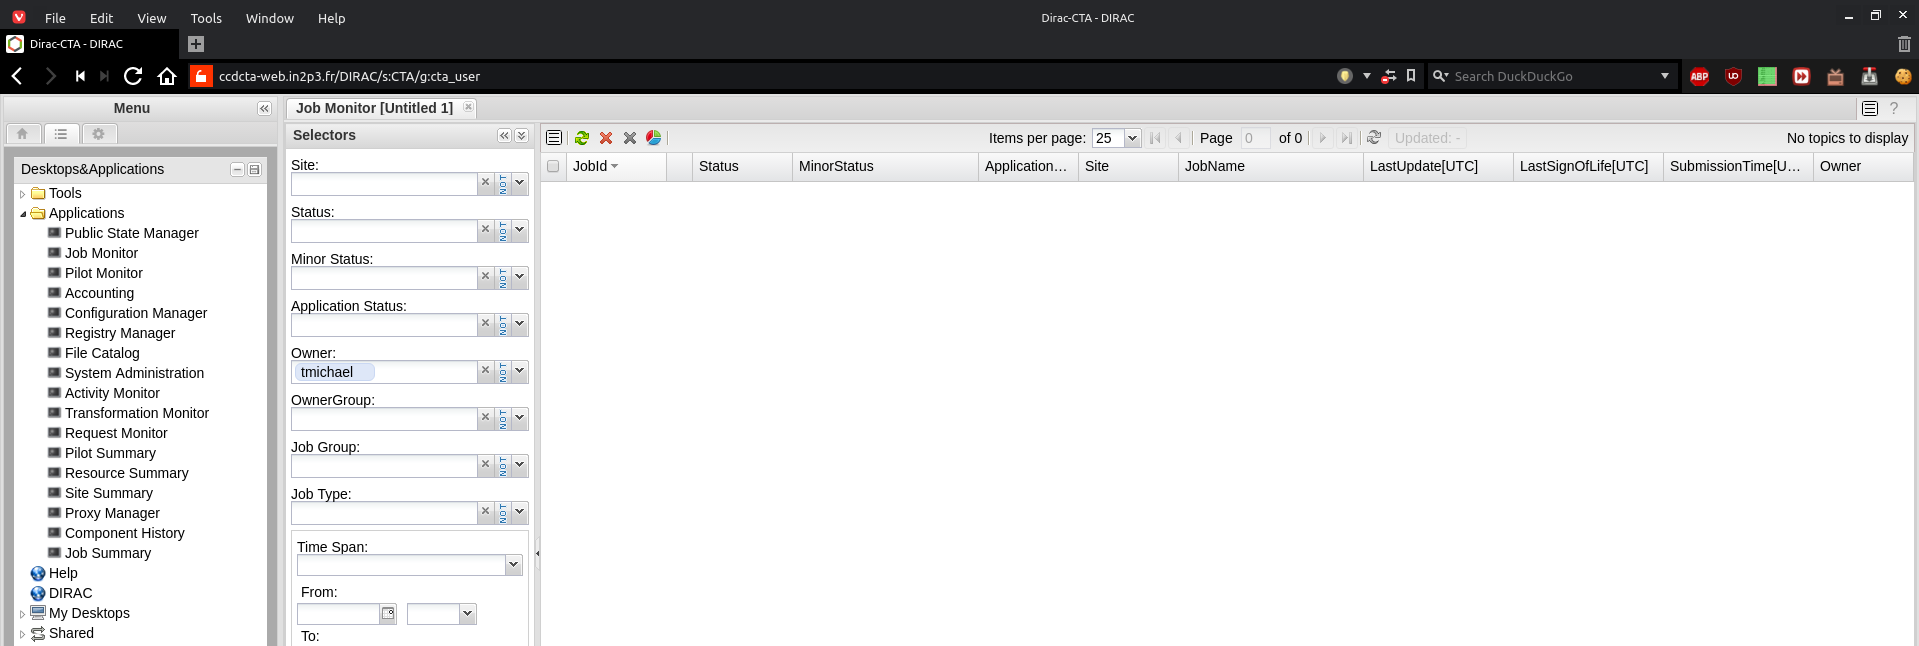
\includegraphics[height=2.5cm]{pics/DIRAC_monitor}

    \end{frame}


%
%     \begin{frame}{Thoughts on Event Weights}
%         \begin{itemize}
%             \item next step: reweighting of MC events to correspond to expected physical
%                 flux (e.g. Crab nebula)
%             \only<2,3>{
%                 \item simple binned approach:
%                     \begin{itemize}
%                         \item construct energy-binned selection efficiencies from MC
%                         \item apply these on the energy-binned histogram of expected
%                             \emph{arriving} events from the source
%                         \item \textrightarrow\ get the number of expected selected events
%                     \end{itemize}
%                 \only<3>{
%                     \item \textbf{but:} it's binned... not optimal (but implemented anyway)
%                 }
%             }
%             \only<4->{
%                 \item instead: event-by-event weight that considers the generator
%                     spectrum:
%                 \item $w(E) = A_\mathrm{gen} \times I_\Theta \times E^\gamma \times I_E
%                     \times T_\mathrm{obs}/ N_\mathrm{gen}$\\ with:
%                     \begin{itemize}
%                         \item $A_\mathrm{gen}$: MC generator Area
%                         \item $I_\Theta = 2 \pi (1-\cos\vartheta)$: angular phase space
%                             factor for diffuse flux
%                         \item $E^\gamma$: considers that MC events have been drawn with an
%                             $E^{-2}$ spectrum
%                         \item $\gamma$: spectral index of the MC generator (here equal 2)
%                         \item $I_E =
%                             (E_\mathrm{max}^{(1-\gamma)} - E_\mathrm{min}^{(1-\gamma)})
%                             / (1-\gamma)$: energy phase space factor
%                         \item $T_\mathrm{obs}$: assumed observation time
%                         \item $N_\mathrm{gen}$: number of generated MC events
%                     \end{itemize}
%                 \item $w(E) \times \varPhi(E)$ gives weight for every MC event so that
%                     their energy distribution looks like the selected events from the
%                     assumed flux $\varPhi$
%             }
%         \end{itemize}
%     \end{frame}
%
%
%     \begin{frame}{Detected (weighted) Events}
%         \ \\
%         \centering
%         % This file was created by matplotlib2tikz v0.6.13.
\begin{tikzpicture}

\definecolor{color0}{rgb}{1,0.647058823529412,0}

\begin{axis}[
xlabel={$E_\mathrm{MC} / \mathrm{TeV}$},
ylabel={expected events in 50.0 h},
xmin=0.00211134817886532, xmax=899.274928164032,
ymin=6.20145233873182, ymax=2090039731.91061,
xmode=log,
ymode=log,
width=\figurewidth,
height=\figureheight,
tick align=outside,
tick pos=left,
x grid style={lightgray!92.026143790849673!black},
y grid style={lightgray!92.026143790849673!black},
legend entries={{proton},{electron},{gamma}},
legend cell align={left},
legend style={draw=white!80.0!black}
]
\addlegendimage{thick, no markers, blue}
\addlegendimage{thick, no markers, red}
\addlegendimage{thick, no markers, color0}
\addplot [thick, blue]
table {%
0.00501658731970781 525890.436305953
0.0075664868484188 3818250.34287699
0.011412484140838 16849942.7512574
0.0172133774728093 49053738.320302
0.0259628281069103 123323833.60541
0.0391595690255296 245949854.141878
0.0590641296838178 412853287.506478
0.0890860523268913 596111961.896461
0.134367927906064 767023550.255601
0.202666293748423 856117908.120863
0.305680285926835 803875716.463921
0.461055637205775 647028487.48175
0.695407294437373 479166934.454113
1.04887841321605 353018434.959394
1.58201666061139 259854649.290884
2.38614569898342 183069823.155587
3.59900842926436 121016332.97422
5.42836159562019 77476868.8166628
8.18756337806838 48290837.3199835
12.3492499327926 30224677.0318213
18.6262953775823 18781076.3215904
28.0939232245735 11445307.0468645
42.3738862800467 6923348.29649925
63.9122640195649 4084670.87777042
96.3984626076187 2391072.42879868
145.397189970735 1351323.74612427
219.301659793434 740724.311494827
330.771303061875 395021.986272812
498.900259269841 208239.02635479
};
\addplot [thick, red]
table {%
0.00380573560867088 57966.2377228595
0.00585001340673278 198483.037202137
0.00899238948207052 1176618.89970735
0.013822715090565 4123563.33940953
0.0212476842618853 7317918.74815696
0.032661028136283 7594871.79730516
0.0502051303930861 9554712.97334596
0.0771731712568687 10955771.6019975
0.118627286000679 7613245.15233149
0.182348771661166 4794182.83427172
0.280298704011029 3480980.97203398
0.430863135268352 2431062.61731149
0.662304315634544 1274754.77551147
1.01806576288997 574732.353893943
1.56492698764273 242577.827853516
2.40553858691859 103857.269799434
3.69769065192668 46972.2299639359
5.68393133733117 22410.1546353549
8.73709525448317 10568.1212988794
13.4302877630741 4956.27778869122
20.6444618200111 2315.06178072095
31.7337804934973 1050.63378868252
48.779805121068 461.954521588981
74.9822224344482 200.058034107089
115.259453522925 82.5730782598257
177.171884149169 35.2142166793346
272.3410147587 15.1395989507437
};
\addplot [thick, color0]
table {%
0.00380573560867088 10451.339722419
0.00585001340673278 50958.8600611574
0.00899238948207052 209053.077893615
0.013822715090565 511864.452915587
0.0212476842618853 718303.43694565
0.032661028136283 744621.657027549
0.0502051303930861 739212.739458969
0.0771731712568687 618142.831888242
0.118627286000679 426649.474264943
0.182348771661166 295661.108610738
0.280298704011029 240765.449362468
0.430863135268352 193232.892029079
0.662304315634544 137717.49658971
1.01806576288997 89258.9045366123
1.56492698764273 54220.5887535168
2.40553858691859 31318.6595734637
3.69769065192668 17623.7947967891
5.68393133733117 10173.9877843391
8.73709525448317 5740.78942457493
13.4302877630741 3200.93190698512
20.6444618200111 1792.67227789201
31.7337804934973 1001.07289448101
48.779805121068 535.660538746975
74.9822224344482 306.72881000489
115.259453522925 160.679740931839
177.171884149169 86.0450838264078
272.3410147587 42.4913428537548
};
\end{axis}

\end{tikzpicture}

%
%     \end{frame}
%
%
%     \begin{frame}{Point-Source Sensitivity}
%         defined as the minimum flux necessary to generate sufficient events in a bin to
%         claim a $5\sigma$ excess according to Li-Ma\\
%         \centering
%         % This file was created by matplotlib2tikz v0.6.13.
\begin{tikzpicture}

\begin{axis}[
xlabel={$E_\mathrm{reco} / \mathrm{TeV}$},
ylabel={$E^2 \varPhi$},  % / \mathrm{\frac{erg}{s\,cm^{2}}}$},
xmin=0.01, xmax=200,
ymin=5e-15, ymax=1e-10,
xmode=log,
ymode=log,
width=\figurewidth,
height=\figureheight,
xtick={0.001,0.01,0.1,1,10,100,1000,10000},
xticklabels={,${10^{-2}}$,${10^{-1}}$,${10^{0}}$,${10^{1}}$,${10^{2}}$,,},
ytick={1e-14,1e-13,1e-12,1e-11},
yticklabels={},
tick align=outside,
tick pos=left,
xmajorgrids,
x grid style={lightgray!92.026143790849673!black},
ymajorgrids,
y grid style={lightgray!92.026143790849673!black},
legend entries={{wavelets},{tailcuts}},
legend style={draw=white!80.0!black},
legend cell align={left}
]
\addlegendimage{thick, darkred}
\addlegendimage{thick, dashed, darkorange}

\addplot [thick, darkred, mark=square*, mark size=1, mark options={solid}]
table {%
0.01 8.97732586049047e-12
0.0158489319246111 1.31346379449665e-12
0.0251188643150958 3.5054272503888e-13
0.0398107170553497 2.20023527007935e-13
0.0630957344480193 1.19125140546455e-13
0.1 5.02638770771275e-14
0.158489319246111 3.68130354957728e-14
0.251188643150958 1.85789074858261e-14
0.398107170553497 1.78405006049022e-14
0.630957344480193 1.75830920476962e-14
0.999999999999999 1.50644459321183e-14
1.58489319246111 1.67622759929585e-14
2.51188643150958 1.63271747349374e-14
3.98107170553497 2.05783453205216e-14
6.30957344480193 2.80892276680632e-14
9.99999999999999 4.29435956270557e-14
15.8489319246111 4.83396995601958e-14
25.1188643150958 7.372821303281e-14
39.8107170553497 1.12993266358001e-13
63.0957344480193 1.34167205548644e-13
99.9999999999998 4.64349558715434e-13
158.489319246111 4.89513853606016e-13
251.188643150958 3.04006128074338e-12
};
\addplot [thick, darkorange, dashed, mark=square*, mark size=1, mark options={solid}]
table {%
0.01 1.0647312887569e-11
0.0158489319246111 5.48328573254468e-13
0.0251188643150958 2.03240768651982e-13
0.0398107170553497 1.85101950259334e-13
0.0630957344480193 1.45644685634984e-13
0.1 9.3584040552676e-14
0.158489319246111 6.39896948769896e-14
0.251188643150958 7.04173738077233e-14
0.398107170553497 4.35544586859766e-14
0.630957344480193 4.77959201023667e-14
0.999999999999999 4.44003948867611e-14
1.58489319246111 4.29734441683112e-14
2.51188643150958 4.96463296384831e-14
3.98107170553497 5.84962814364508e-14
6.30957344480193 7.60528735010101e-14
9.99999999999999 7.35841968805884e-14
15.8489319246111 9.12710099525779e-14
25.1188643150958 1.35556556243919e-13
39.8107170553497 1.86570122576284e-13
63.0957344480193 1.94358919798559e-13
99.9999999999998 6.49662441457101e-13
158.489319246111 4.67302879193594e-13
251.188643150958 4.61054256328862e-12
};

\end{axis}

\end{tikzpicture}

%
%     \end{frame}


    \begin{frame}{Effective Areas}{after reconstruction}
        \centering
        \setlength{\figureheight}{7cm}
        \setlength{\figurewidth}{.75\textwidth}
        % This file was created by matplotlib2tikz v0.6.13.
\begin{tikzpicture}

\definecolor{color0}{rgb}{1,0.647058823529412,0}

\begin{axis}[
title={Effective Areas -- wavelets},
xlabel={$E_\mathrm{MC} / \mathrm{TeV}$},
ylabel={$A_\mathrm{eff} / \mathrm{m}^2$},
xmin=0.00211134817886532, xmax=899.274928164032,
ymin=0.0200562006408878, ymax=21315876.6110353,
xmode=log,
ymode=log,
width=\figurewidth,
height=\figureheight,
tick align=outside,
tick pos=left,
x grid style={lightgray!92.026143790849673!black},
y grid style={lightgray!92.026143790849673!black},
legend cell align={left},
legend entries={{proton},{electron},{gamma}},
legend style={at={(0.97,0.03)}, anchor=south east, draw=white!80.0!black}
]
\addlegendimage{thick, blue}
\addlegendimage{thick, red}
\addlegendimage{thick, color0}
\addplot [thick, blue, mark=triangle*, mark size=1, mark options={solid}]
table {%
0.00501658731970781 0.0515872115391983
0.0075664868484188 0.735212479093373
0.011412484140838 6.32776872509162
0.0172133774728093 36.4064257758529
0.0259628281069103 180.726556461153
0.0391595690255296 711.768108411842
0.0590641296838178 2362.10928929799
0.0890860523268913 6742.95260013528
0.134367927906064 17167.8702085258
0.202666293748423 37875.7158431283
0.305680285926835 70256.8940262742
0.461055637205775 111877.481033063
0.695407294437373 164161.115149263
1.04887841321605 240015.576158033
1.58201666061139 350229.677073928
2.38614569898342 488821.916478075
3.59900842926436 640364.417600073
5.42836159562019 812583.950156802
8.18756337806838 1004772.41049069
12.3492499327926 1246754.7620259
18.6262953775823 1536880.27677009
28.0939232245735 1857125.44306546
42.3738862800467 2228424.35903565
63.9122640195649 2605383.43837
96.3984626076187 3024265.02480512
145.397189970735 3386858.29321881
219.301659793434 3683857.93454781
330.771303061875 3897760.78680094
498.900259269841 4075281.68984972
};
\addplot [thick, red, mark=triangle*, mark size=1, mark options={solid,rotate=180}]
table {%
0.00380573560867088 0.489378585794369
0.00585001340673278 4.63888581792463
0.00899238948207052 70.9215183982081
0.013822715090565 629.813135603027
0.0212476842618853 2799.62949586061
0.032661028136283 7402.97685086241
0.0502051303930861 24110.5042087212
0.0771731712568687 66179.359327251
0.118627286000679 104824.683579382
0.182348771661166 144989.883932608
0.280298704011029 236478.66184337
0.430863135268352 401900.223081299
0.662304315634544 579083.127001572
1.01806576288997 784636.900139965
1.56492698764273 1007626.7842713
2.40553858691859 1239759.25368931
3.69769065192668 1515806.91314059
5.68393133733117 1896795.12633557
8.73709525448317 2314037.32019204
13.4302877630741 2815149.56324942
20.6444618200111 3394211.90630118
31.7337804934973 3988144.38024897
48.779805121068 4521486.82992411
74.9822224344482 5044344.30162532
115.259453522925 5430728.90020596
177.171884149169 5991794.36277805
272.3410147587 6595482.80226556
};
\addplot [thick, color0, mark=square*, mark size=1, mark options={solid}]
table {%
0.00380573560867088 104.292050900348
0.00585001340673278 968.967668287292
0.00899238948207052 7533.63446475569
0.013822715090565 34801.9278898888
0.0212476842618853 92235.0817647462
0.032661028136283 181879.261476612
0.0502051303930861 343712.448130601
0.0771731712568687 545266.876795822
0.118627286000679 716156.292113538
0.182348771661166 947681.239601108
0.280298704011029 1474390.96605585
0.430863135268352 2250212.75430304
0.662304315634544 3049679.78686871
1.01806576288997 3762784.43176057
1.56492698764273 4351856.953396
2.40553858691859 4785330.1640352
3.69769065192668 5134925.18085367
5.68393133733117 5645265.93032058
8.73709525448317 6068102.09381617
13.4302877630741 6449984.10416134
20.6444618200111 6891702.22033018
31.7337804934973 7313054.86553936
48.779805121068 7479859.13887663
74.9822224344482 8172117.46066107
115.259453522925 8110189.35283733
177.171884149169 8287237.96831868
272.3410147587 7817630.70205645
};
\end{axis}

\end{tikzpicture}


    \end{frame}




    \begin{frame}{Summary}
        \begin{itemize}
            \item data pipeline from reading of the MC files to IRFs and differential
                sensitivity fully implemented
            \item (almost) completely written in python
            \item many things unmentioned (pyhessio, camera calibration, ImPACT,
                muon reconstruction, ...)
            \item still ``one or two'' things to do

            \bigskip
            \item image cleaning with wavelet outperforms two-stage tailcuts:\\
                better angular/position resolution, better acceptance, better sensitivity
            \item will show more of that tomorrow at ASWG session

        \end{itemize}

    \end{frame}



    \backup[hide]{
        \frame{
            not shown
        }
    }

\end{document}


• effective area after reconstruction + 68 % PSF
• what is missing? / experience of problems
  • data format
  • database access
  • coordinate robust
